%\documentclass[mathserif,serif]{beamer}
\documentclass{beamer}
\usepackage[utf8]{inputenc}
\usepackage[T1]{fontenc}
\usetheme{Warsaw}
\usepackage{graphicx}
\graphicspath{ {../thesis/images/} }

%\usepackage{caption}
%\captionsetup{font=scriptsize,labelfont=scriptsize}
%\captionsetup[figure]{labelformat=empty}

%\usepackage{float}
%\usepackage{multicol}
 
\titlegraphic{\vspace{-1cm}\flushleft
\includegraphics[scale=0.3]{ufrgs}}
  
\title[]{Estimativa da produção de energia de um parque eólico por meio de modelo estocástico}
\author[]{Diogo Daniel Panda Friggo}
\institute
{
	Universidade Federal do Rio Grande do Sul\newline\newline
	Orientador: Carlo Requião da Cunha
}

\date{Porto Alegre, 2019}
    
%\setbeamertemplate{navigation symbols}{}

\begin{document}
    
\begin{frame}
	\titlepage
\end{frame}

\begin{frame}
	\frametitle{Comparação entre a composição da matriz energética brasileira no ano de 2017 (esquerda) e no ano de 2018 (direita)}
	\begin{figure}
		\centering
		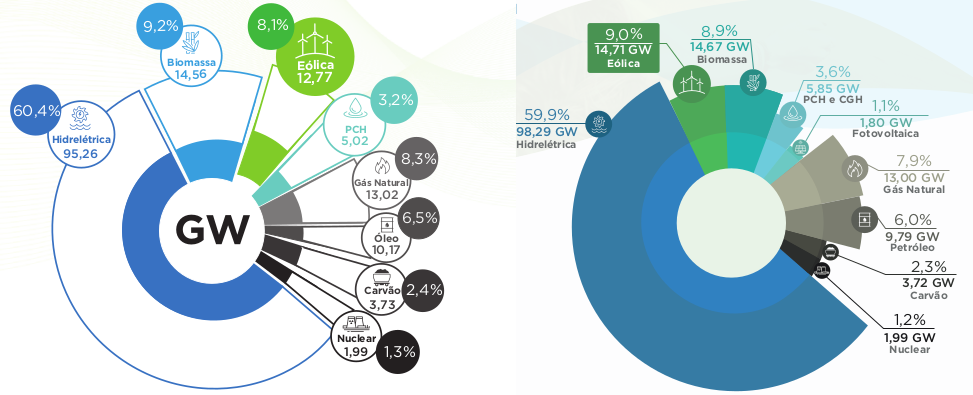
\includegraphics[width=\textwidth]{abe_2017_2018}
		\caption{Comparação entre a composição da matriz energética brasileira no ano de 2017 (esquerda) e no ano de 2018 (direita)}
	\end{figure}
\end{frame}

\begin{frame}
	\frametitle{Ranking de capacidade eólica instalada acumulada}
	\begin{figure}
		\centering
		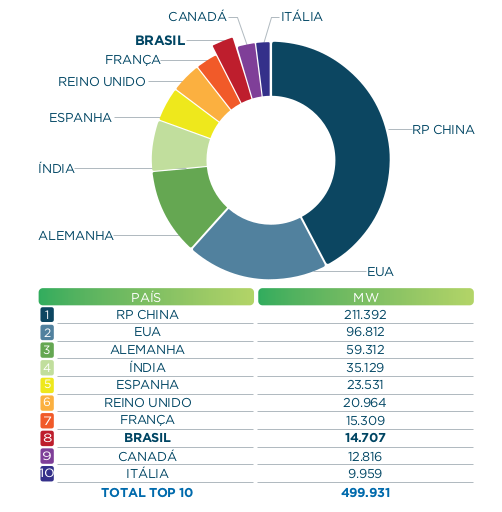
\includegraphics[width=\textwidth]{abe_maiores_produtores}
		\caption{Ranking de capacidade eólica instalada acumulada}
	\end{figure}
\end{frame}

\begin{frame}
	\frametitle{Evolução da capacidade instalada de parques eólicos no Brasil}
	\begin{figure}
		\centering
		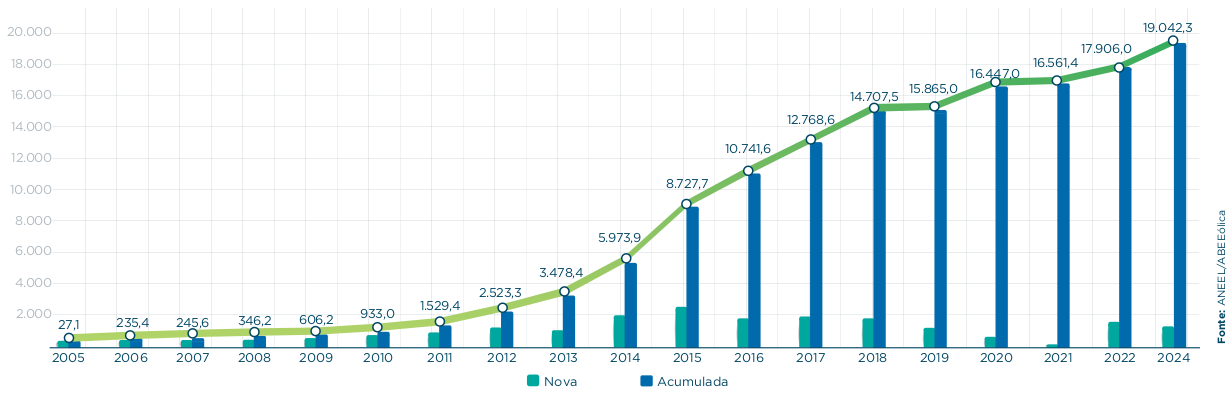
\includegraphics[width=\textwidth]{abe_evolucao_capacidade_instalada}
		\caption{Evolução da capacidade instalada de parques eólicos no Brasil}
	\end{figure}
\end{frame}

\begin{frame}
	\frametitle{Wikimedia Commons}
	\begin{figure}
		\centering
		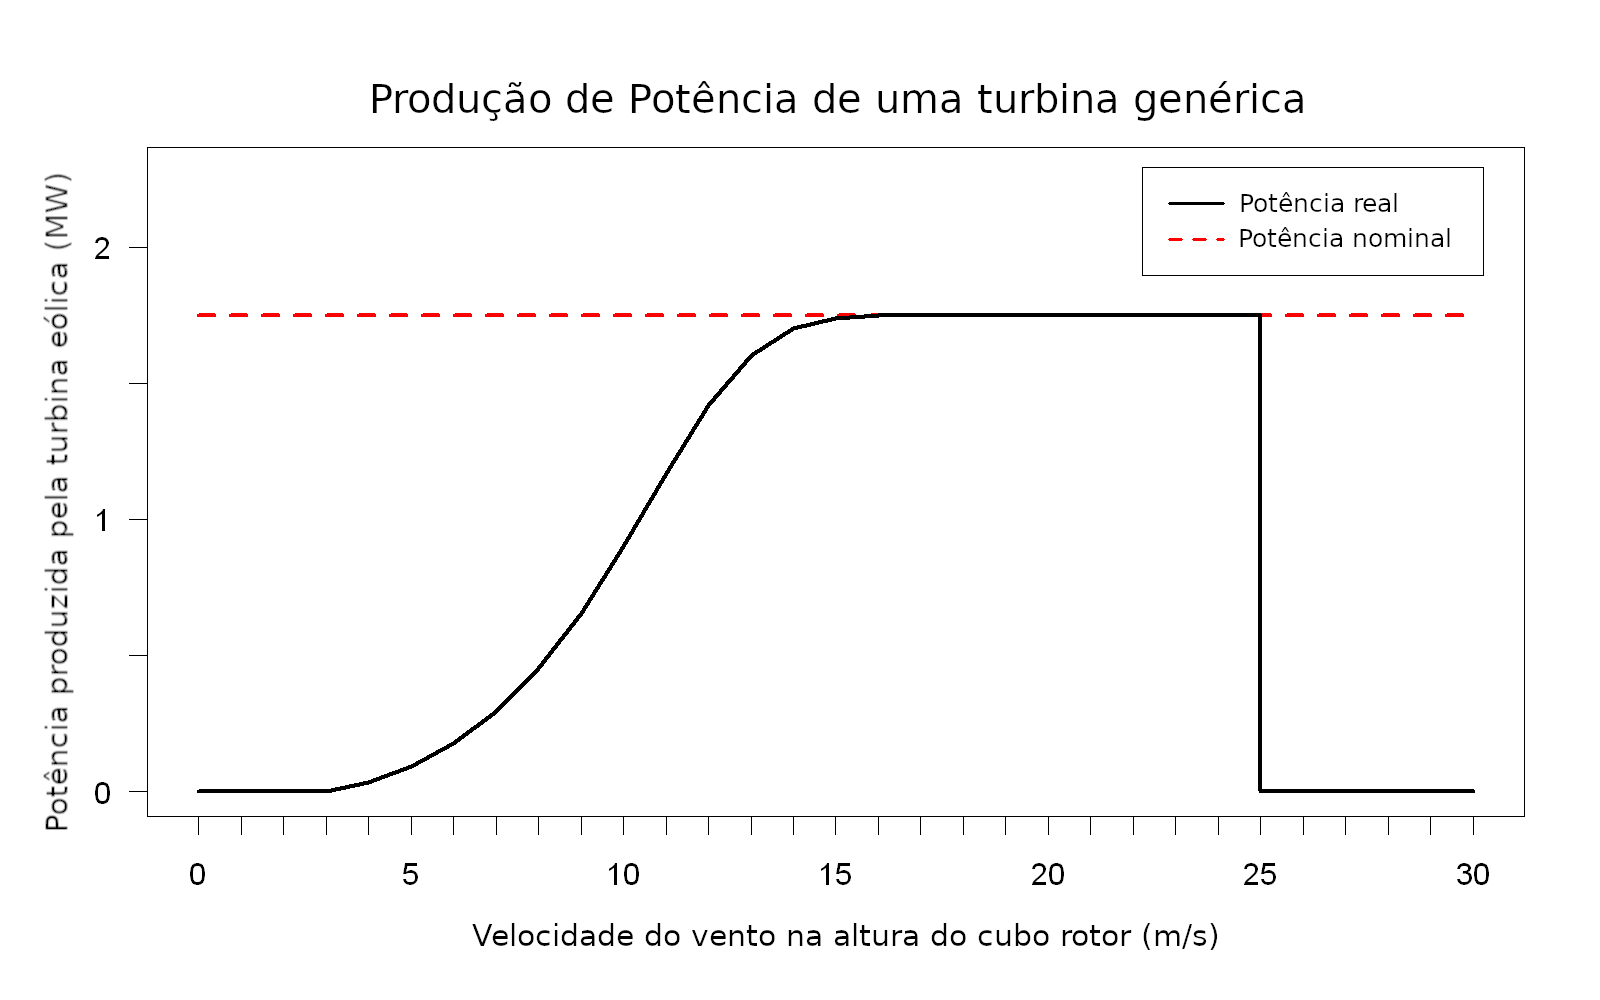
\includegraphics[width=\textwidth]{powercurve}
		\caption{Wikimedia Commons}
	\end{figure}
\end{frame}

\begin{frame}
	\frametitle{era5.}
	\begin{figure}
		\centering
		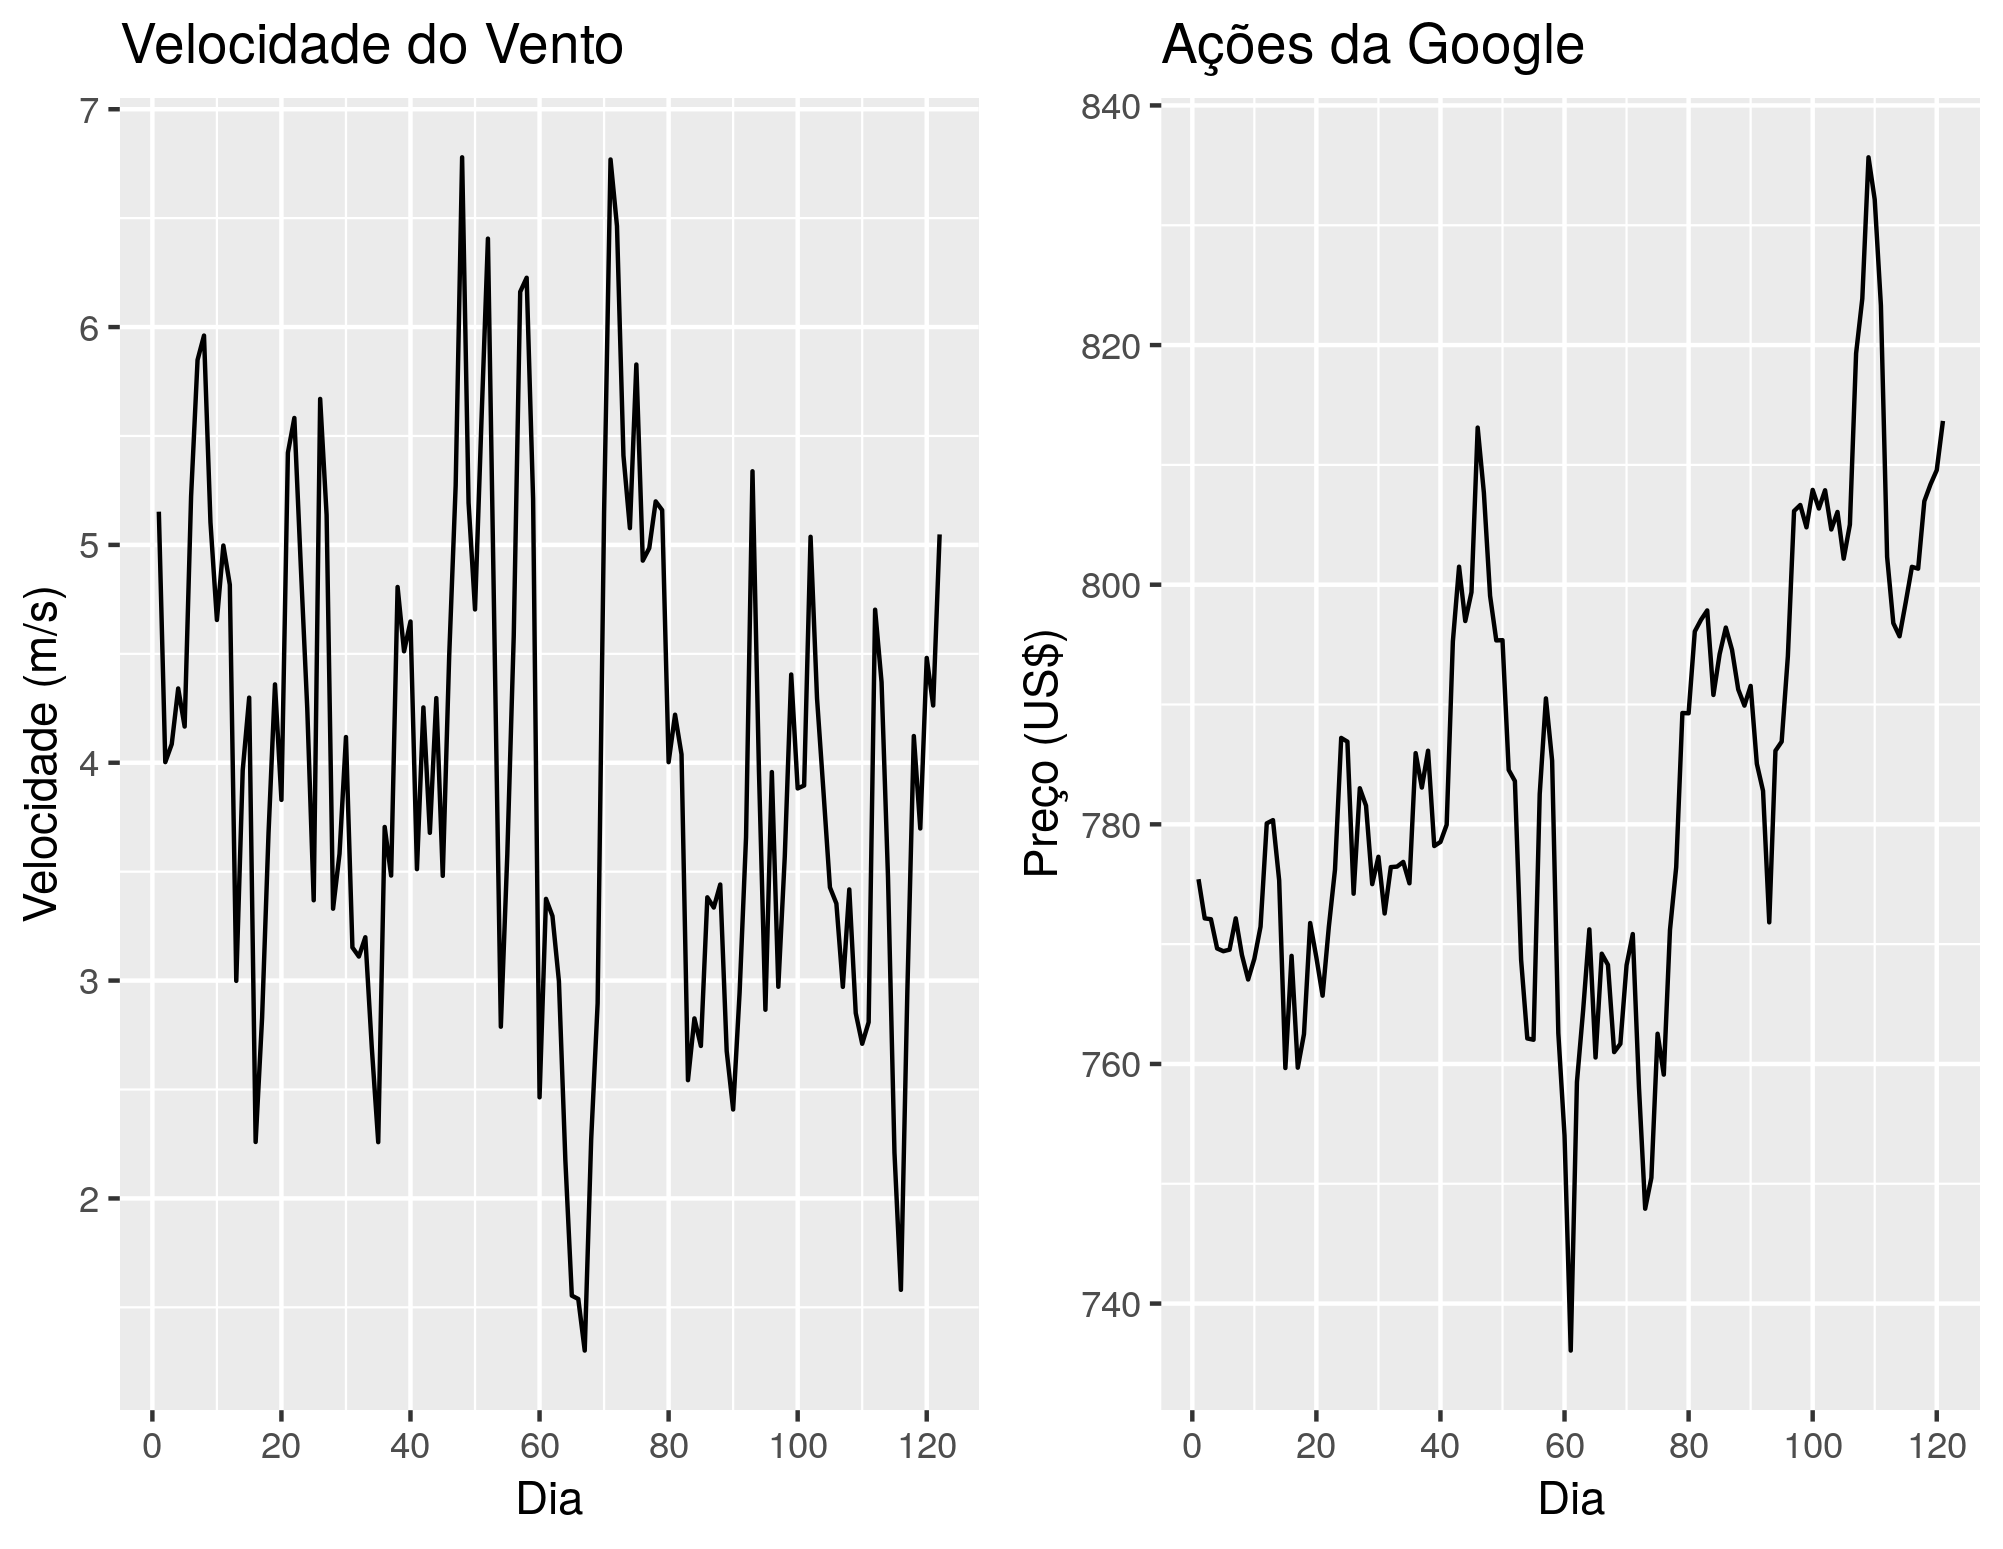
\includegraphics[width=\textwidth]{wind_money}
		\caption{era5.}
	\end{figure}
\end{frame}

\begin{frame}
	\frametitle{Chapada}
	\begin{figure}
		\centering
		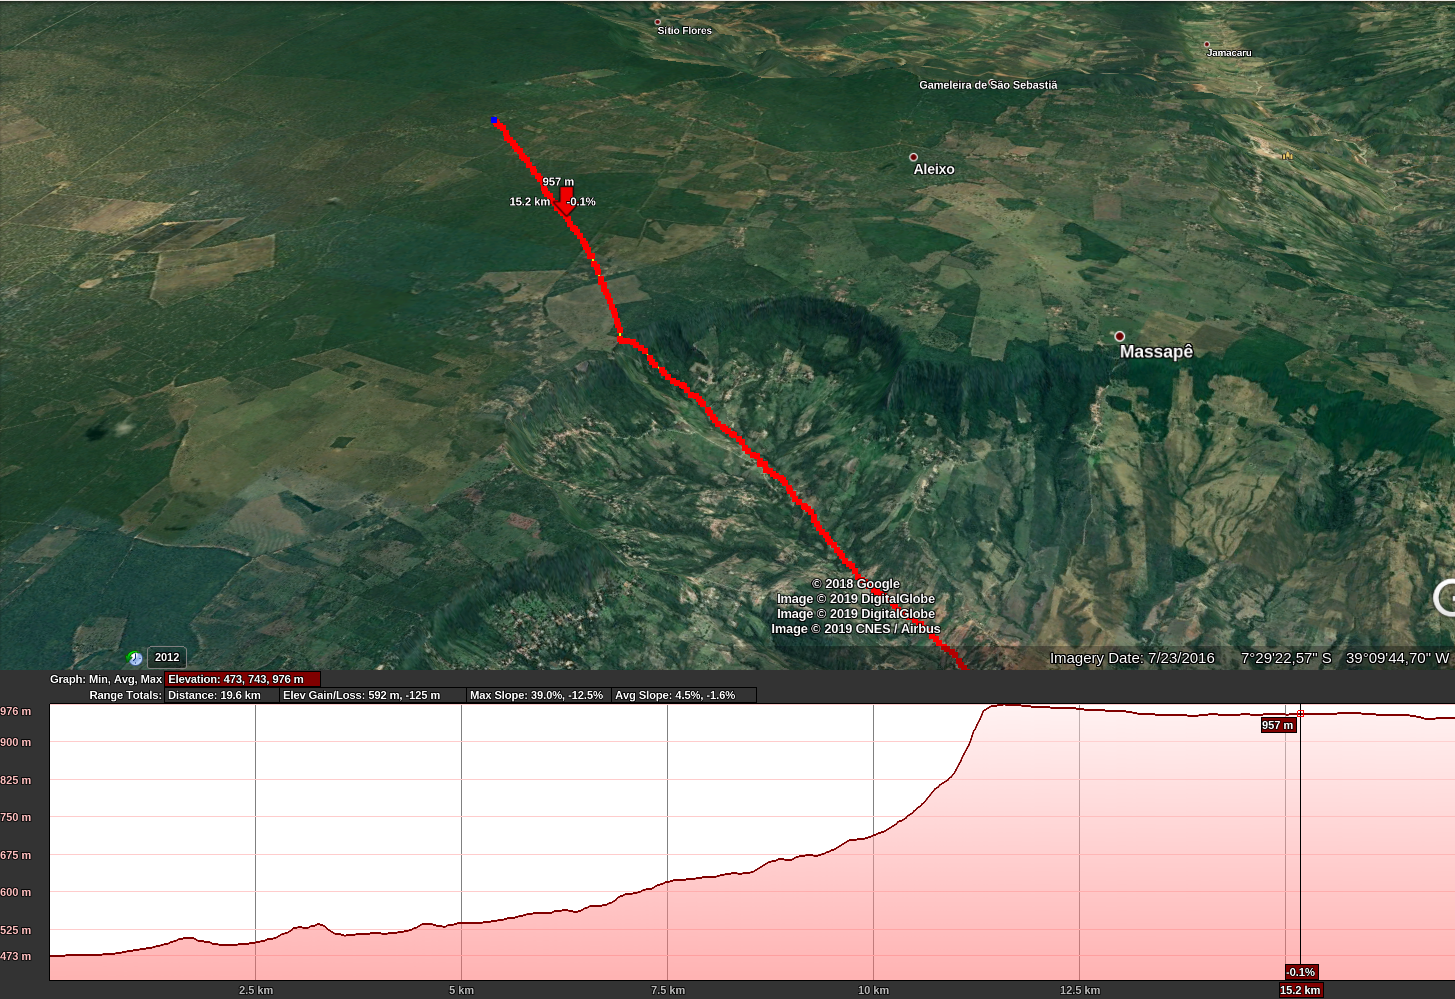
\includegraphics[width=\textwidth]{elevation2}
		\caption{Chapada}
	\end{figure}
\end{frame}

\begin{frame}
	\frametitle{Variação da elevação na direção preferencial de escoamento do vento.}
	\begin{figure}
		\centering
		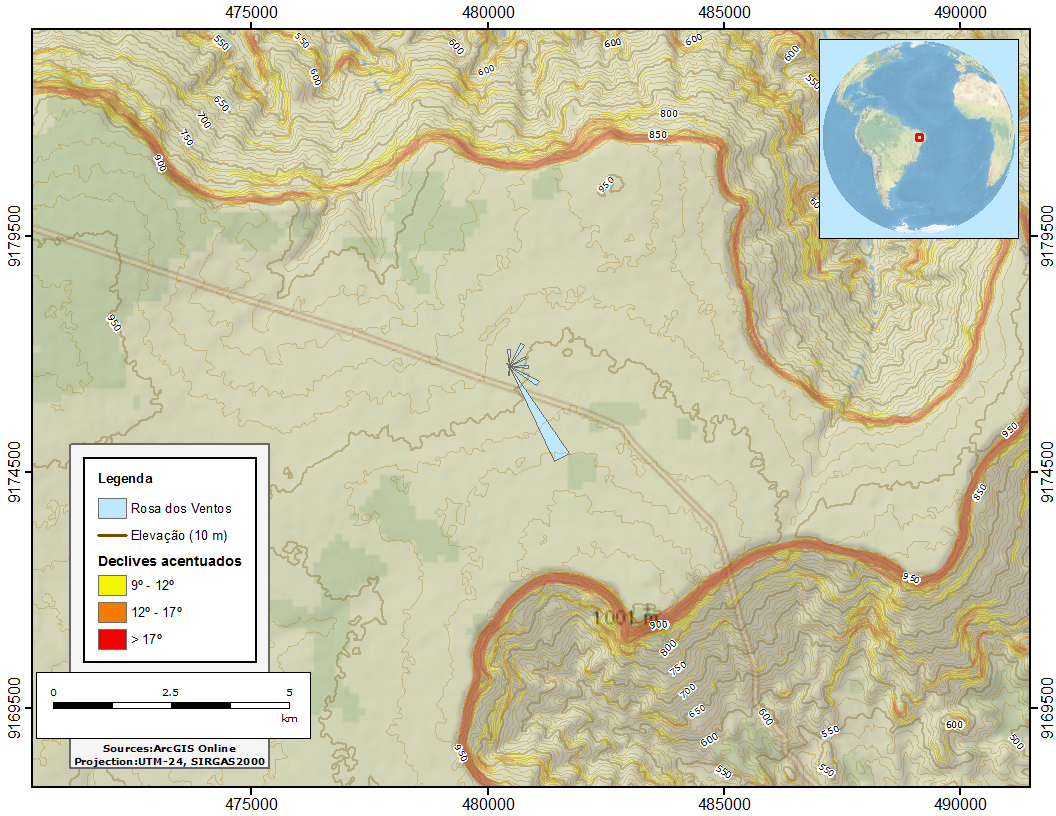
\includegraphics[width=\textwidth]{arcmap}
		\caption{Variação da elevação na direção preferencial de escoamento do vento.}
	\end{figure}
\end{frame}

\begin{frame}
	\frametitle{Alguns nós da série ERA 5 ao sul do Ceará, Brasil.\newline Google earth V 7.3.2.5776. (14 de Dezembro, 2015). Rio Grande do Sul, Brasil.}
	\begin{figure}
		\centering
		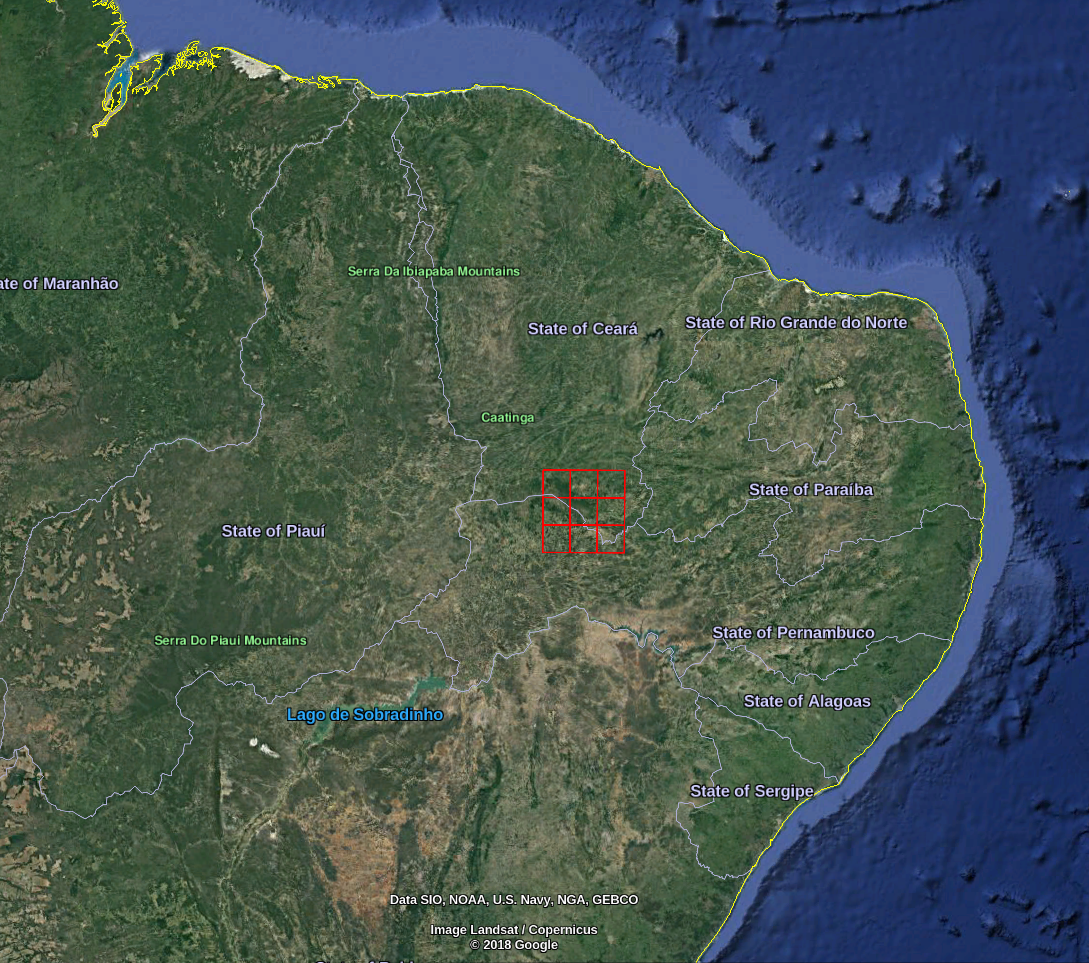
\includegraphics[width=\textwidth]{era5nodes}
		\caption{Alguns nós da série ERA 5 ao sul do Ceará, Brasil.\newline Google earth V 7.3.2.5776. (14 de Dezembro, 2015). Rio Grande do Sul, Brasil.}
	\end{figure}
\end{frame}

\begin{frame}
	\frametitle{Velocidade do vento registrada por satélite na região de interesse nos anos de 2017 e 2018}
	\begin{figure}
		\centering
		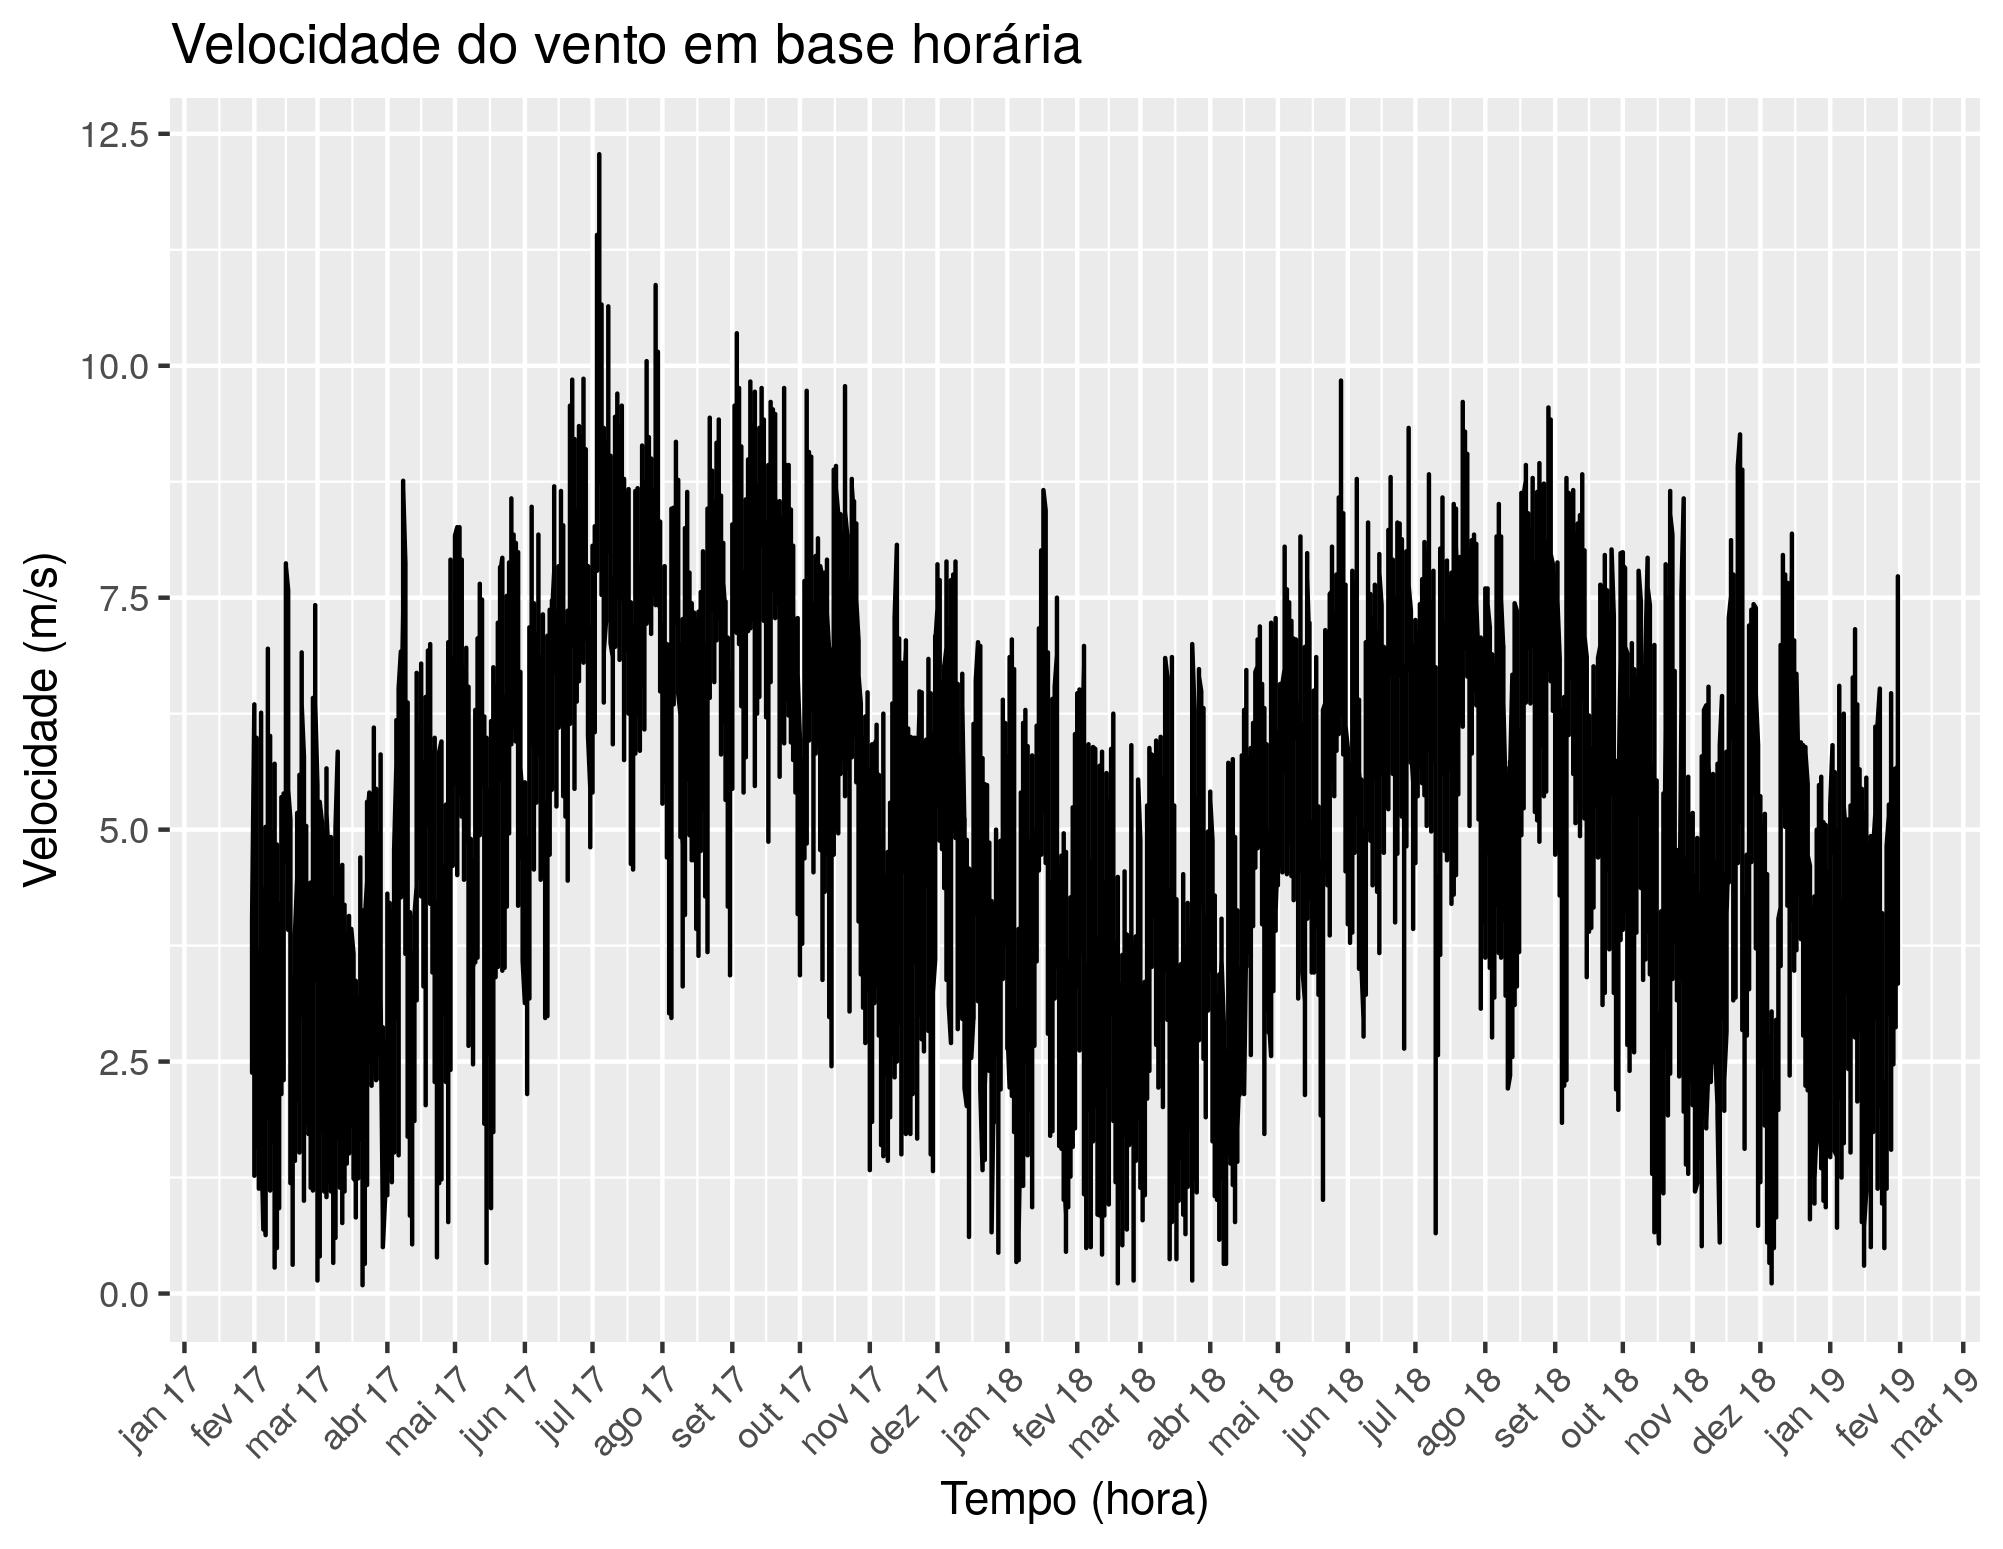
\includegraphics[width=\textwidth]{entire_series_hourly_basis.png}
		\caption{Velocidade do vento registrada por satélite na região de interesse nos anos de 2017 e 2018}
	\end{figure}
\end{frame}

\begin{frame}
	\frametitle{Histograma de velocidades do nó noroeste da série de dados modelo.}
	\begin{figure}
		\centering
		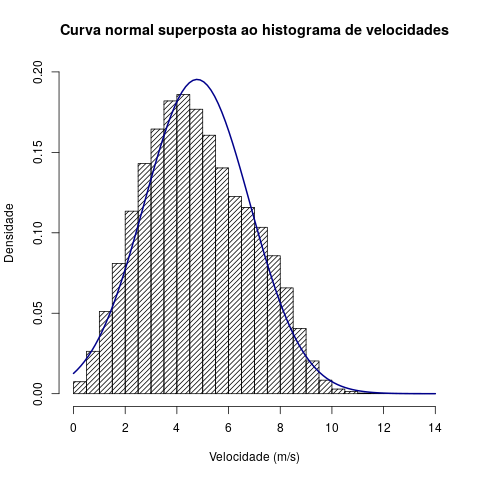
\includegraphics[width=\textwidth]{normal_overlay}
		\caption{Histograma de velocidades do nó noroeste da série de dados modelo.}
	\end{figure}
\end{frame}

\begin{frame}
	\frametitle{Gráfico de Cullen e Frey para os dados do nó noroeste da série de dados modelo.}
	\begin{figure}
		\centering
		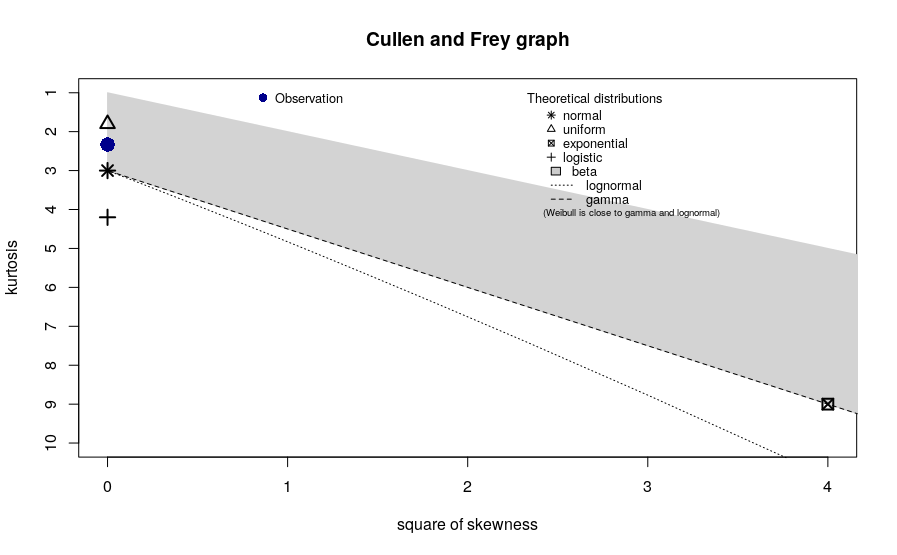
\includegraphics[width=\textwidth]{cullen}
		\caption{Gráfico de Cullen e Frey para os dados do nó noroeste da série de dados modelo.}
	\end{figure}
\end{frame}

\begin{frame}
	\frametitle{Rosa dos ventos}
	\begin{figure}
		\centering
		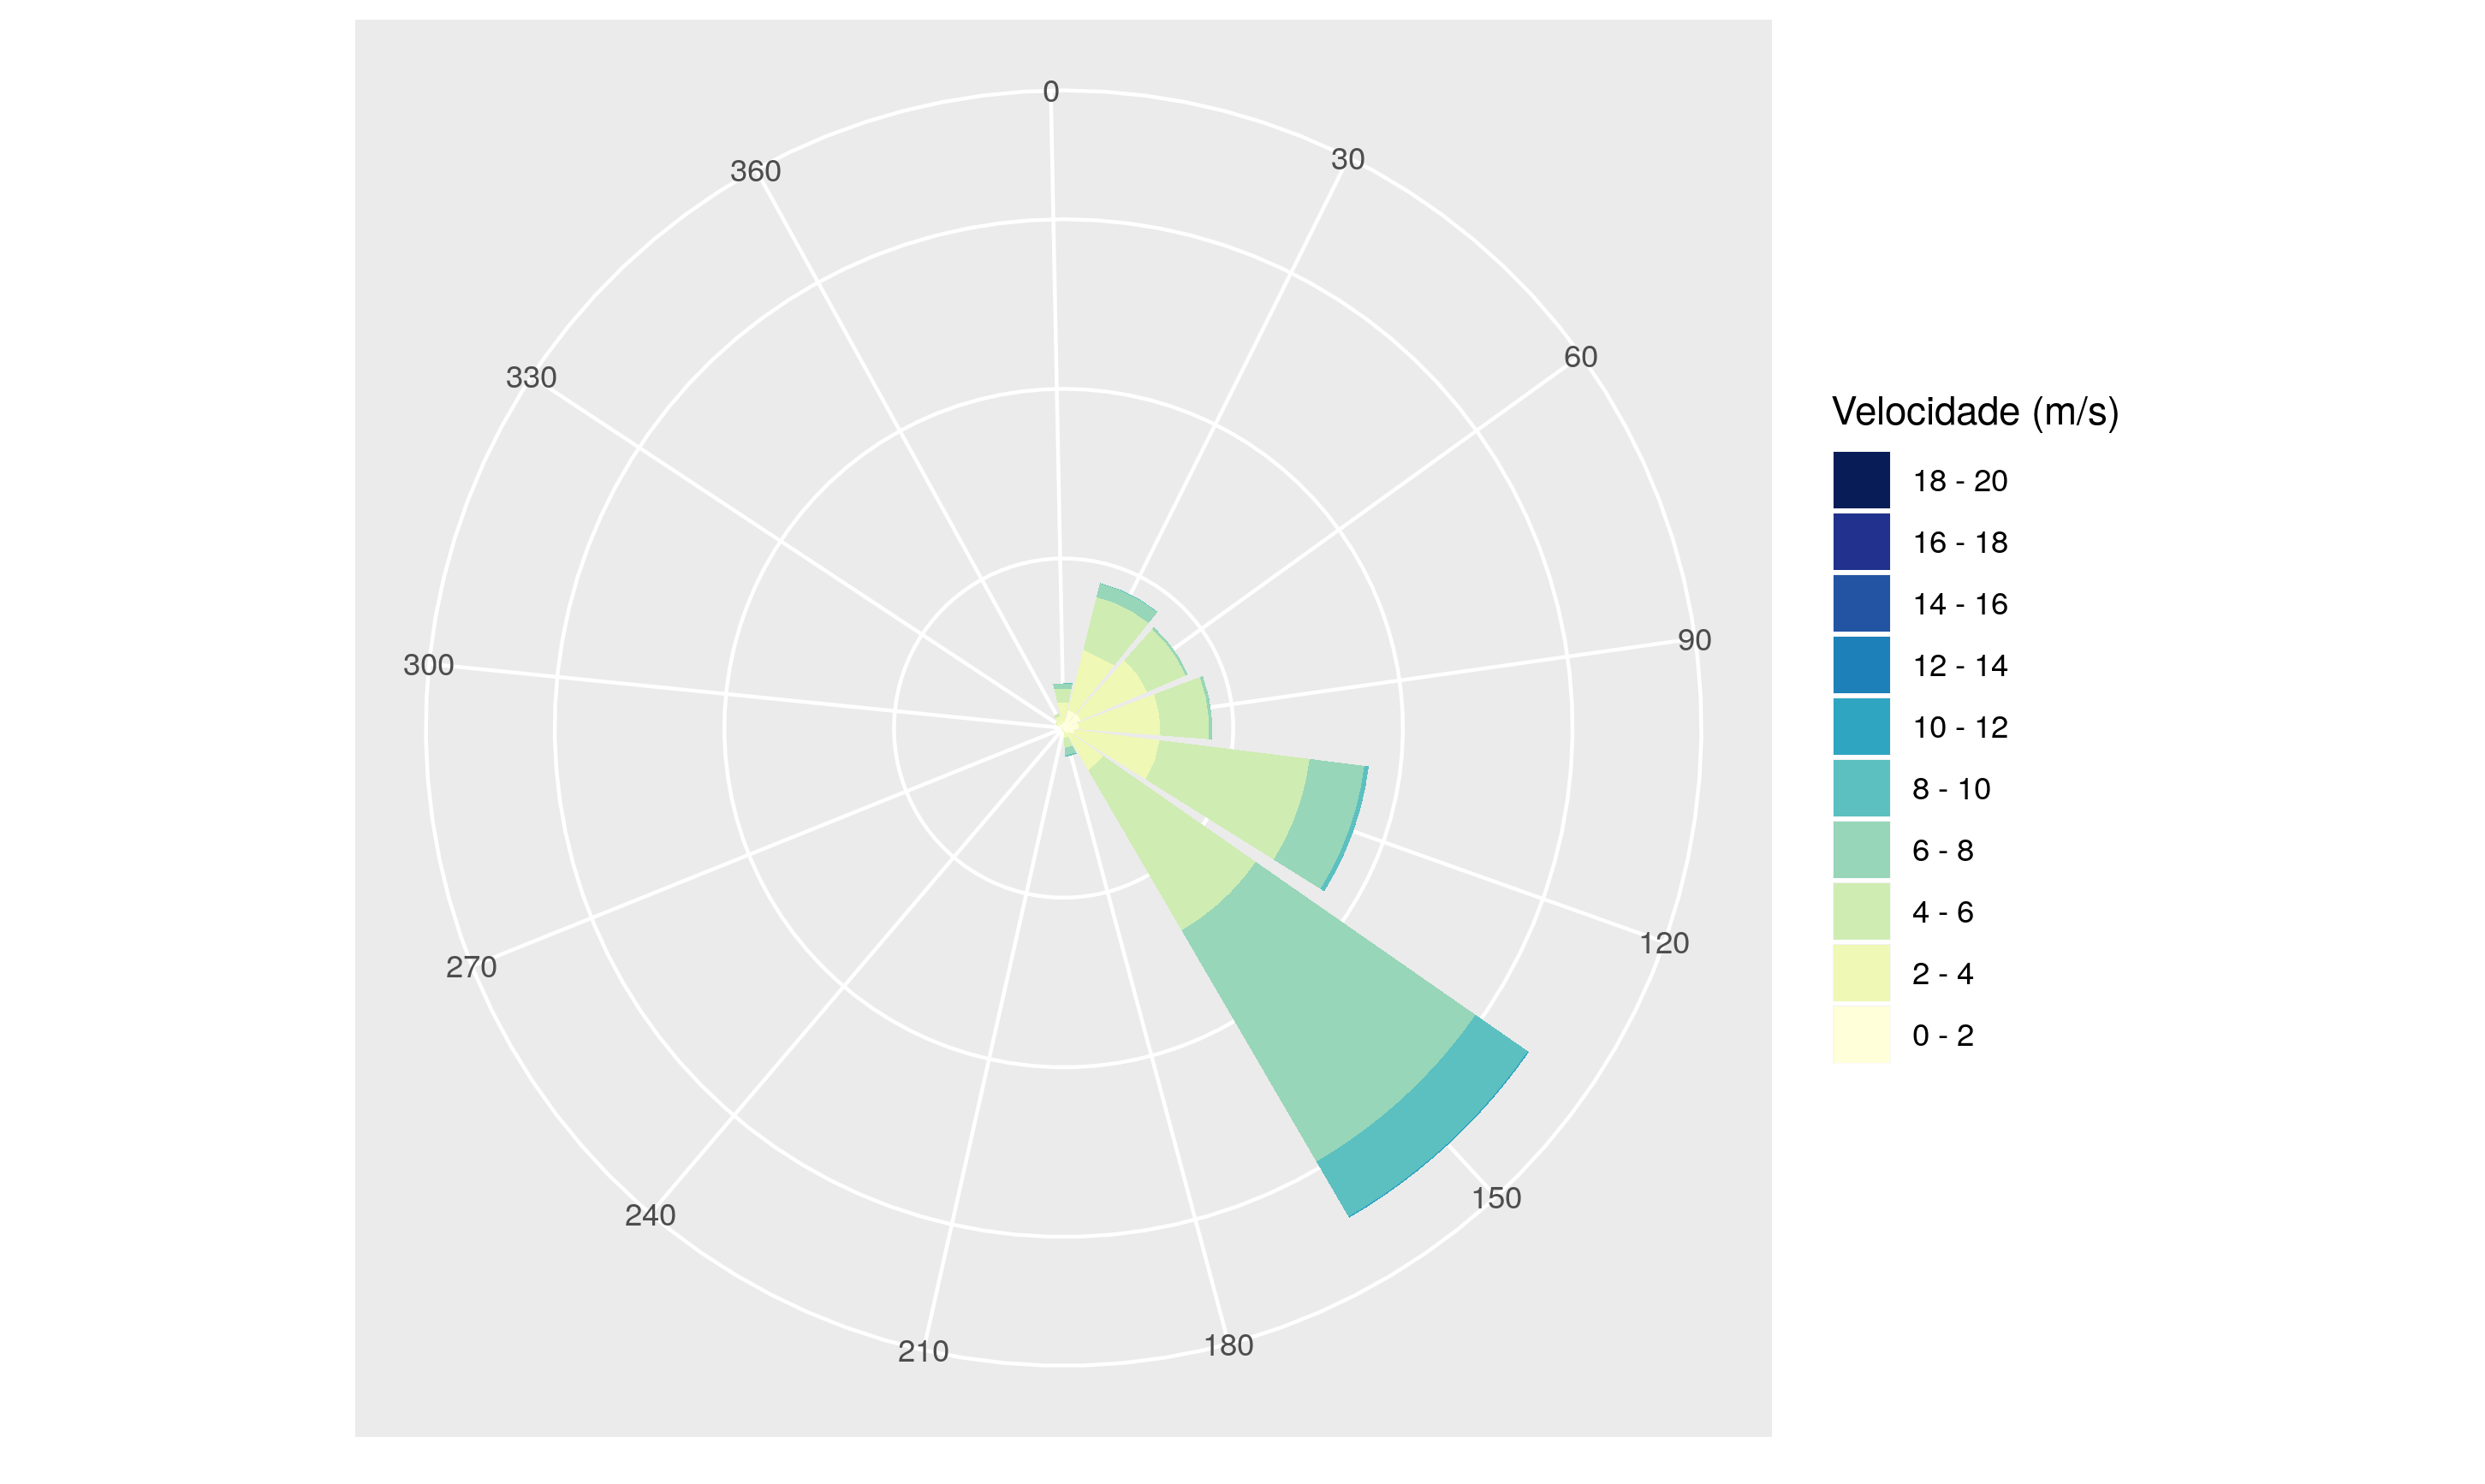
\includegraphics[width=\textwidth]{windrose}
		\caption{Rosa dos ventos}
	\end{figure}
\end{frame}

\begin{frame}
	\frametitle{Chapada}
	\begin{figure}
		\centering
		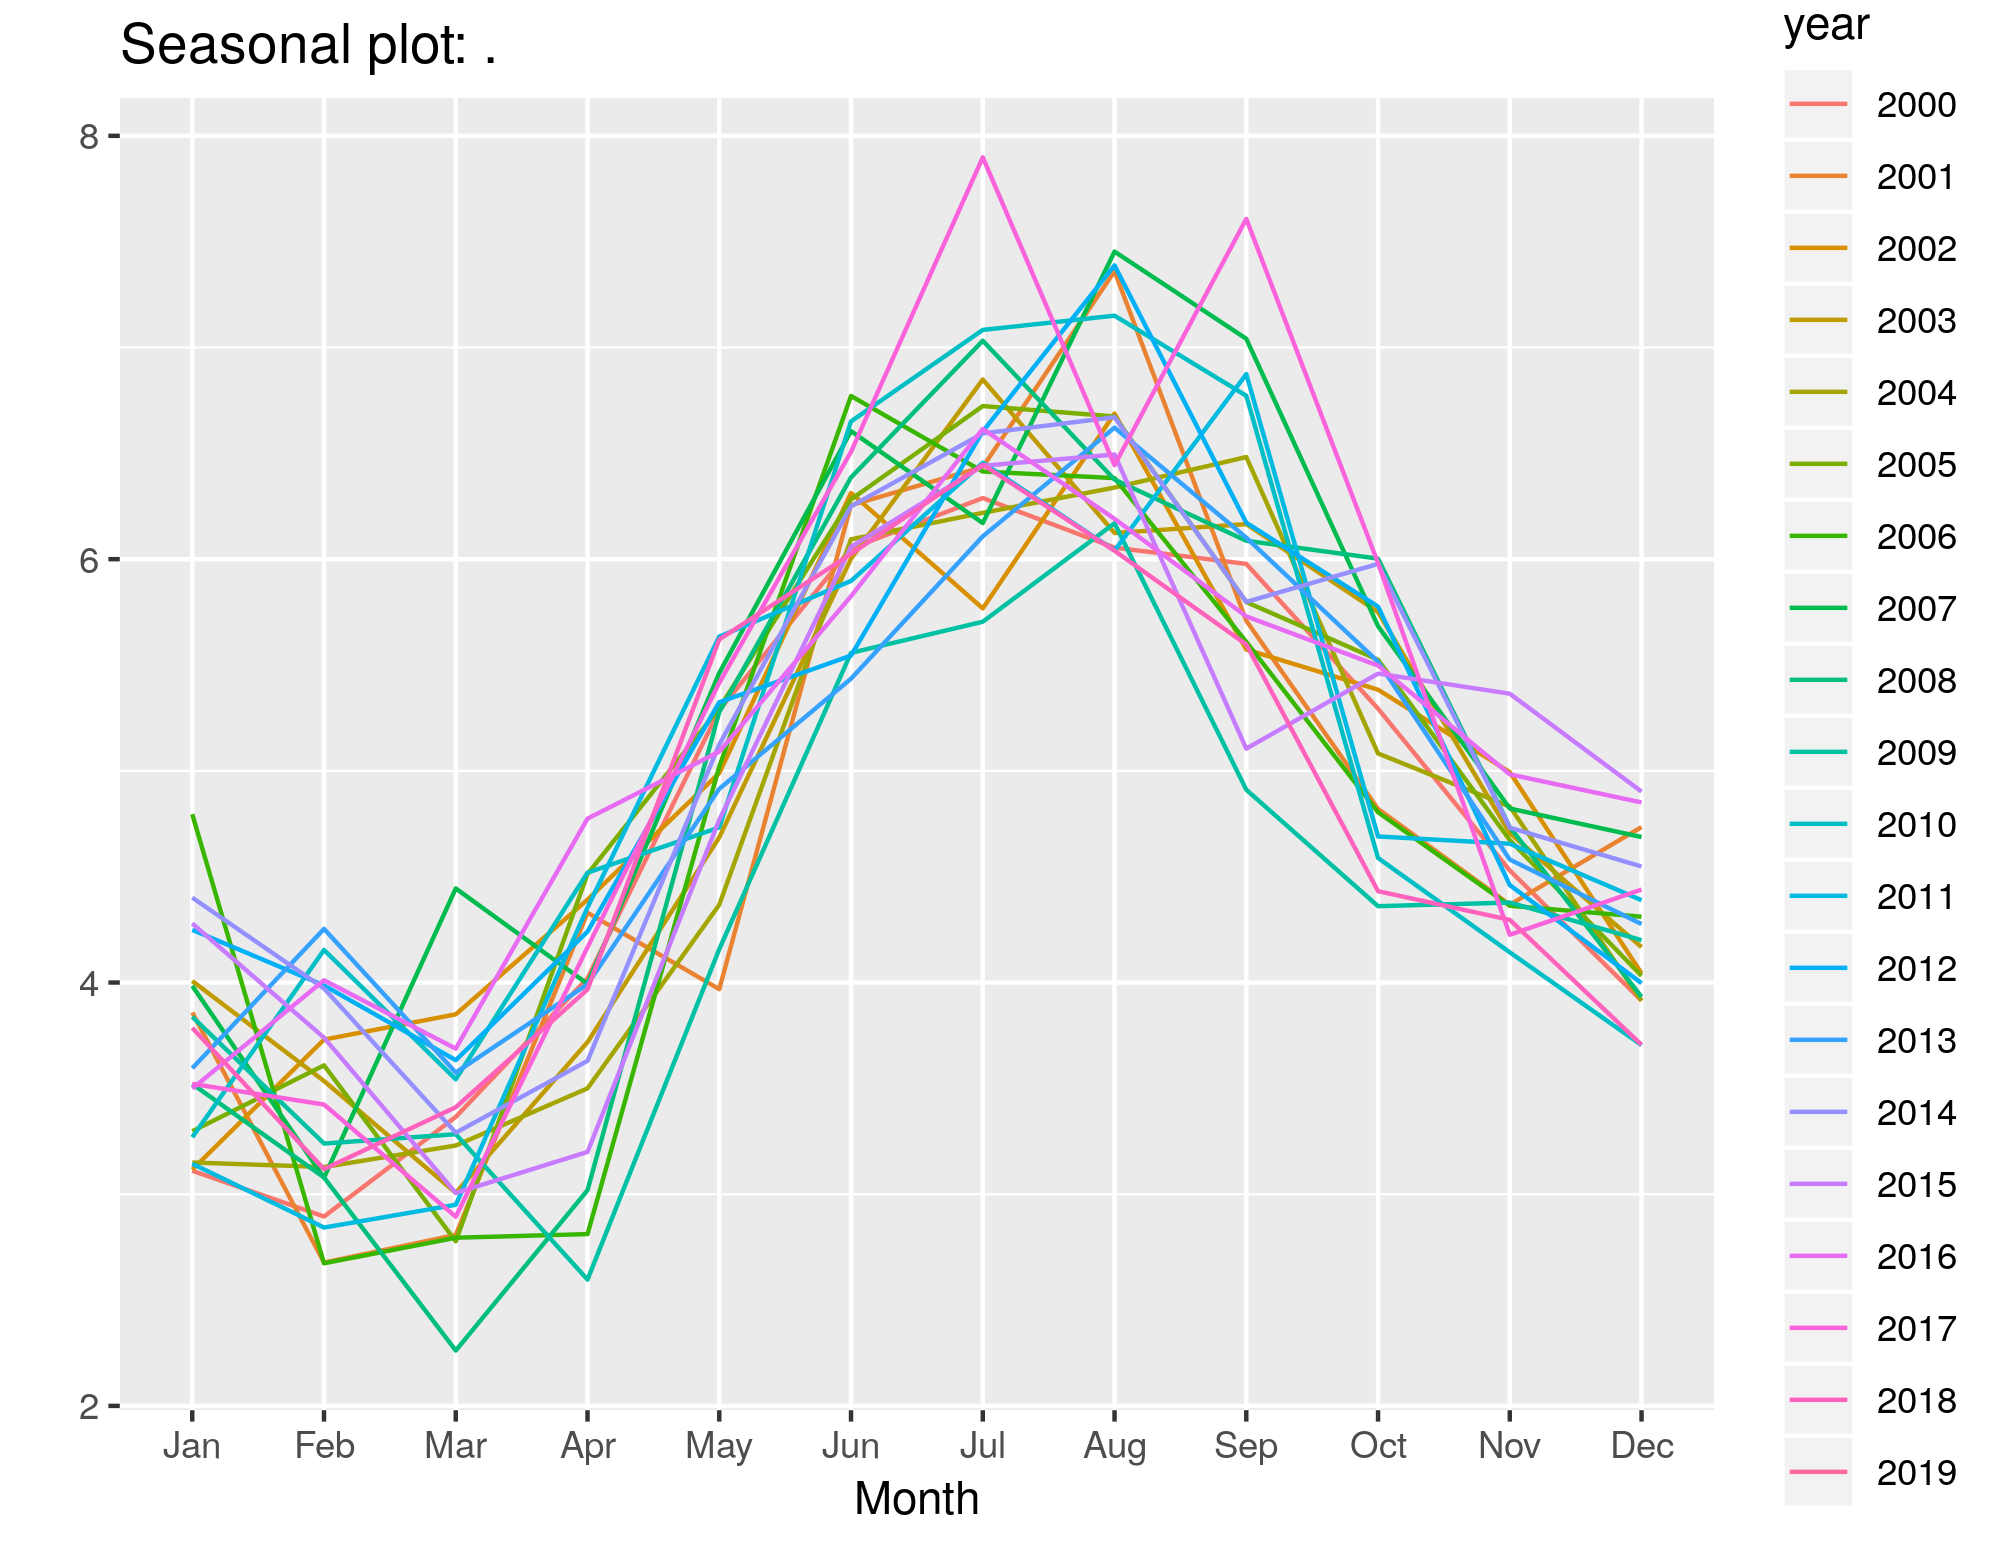
\includegraphics[width=\textwidth]{season_plot}
		\caption{Chapada}
	\end{figure}
\end{frame}

\begin{frame}
	\frametitle{Chapada}
	\begin{figure}
		\centering
		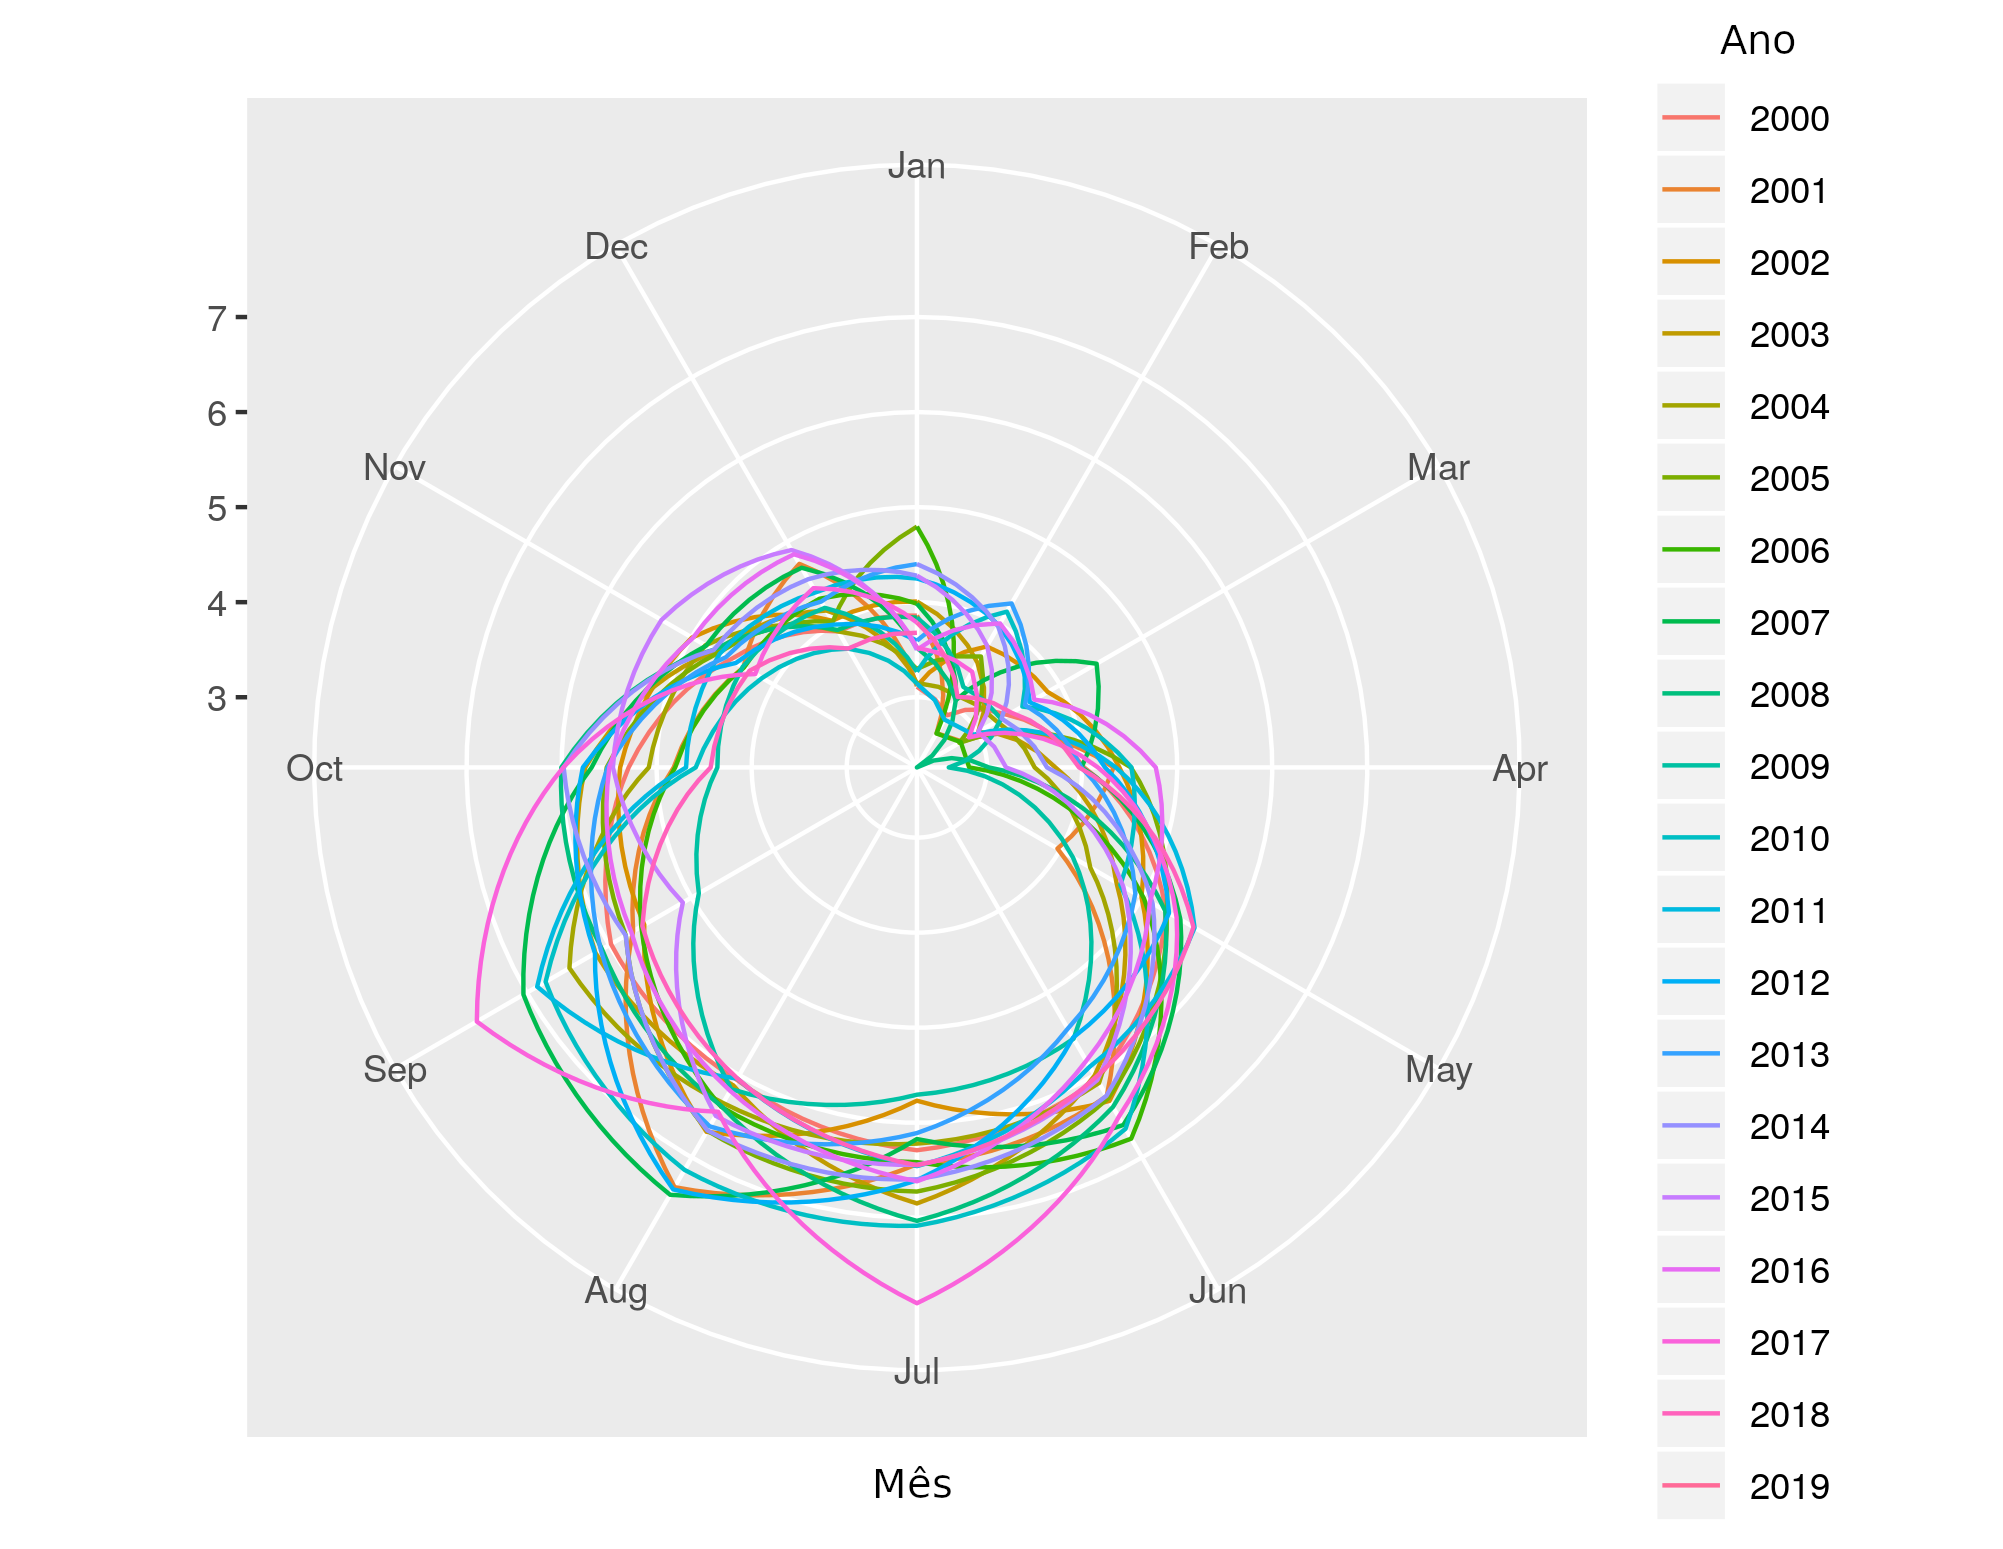
\includegraphics[width=\textwidth]{season_plot_polar}
		\caption{Chapada}
	\end{figure}
\end{frame}

\begin{frame}
	\frametitle{O método de Box-Jenkins.}
	\begin{figure}
		\centering
		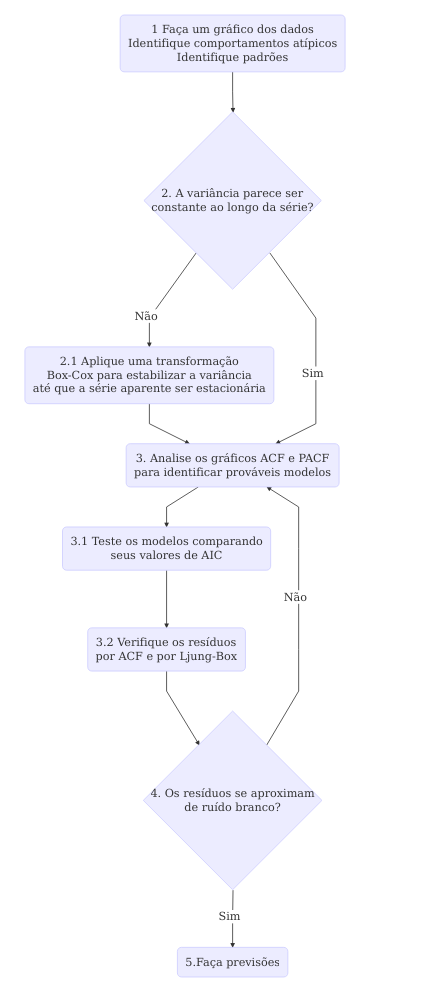
\includegraphics[width=\textwidth]{boxjenkins}
		\caption{O método de Box-Jenkins.}
	\end{figure}
\end{frame}

\begin{frame}
	\frametitle{Últimos dois anos da série de vento}
	\begin{figure}
		\centering
		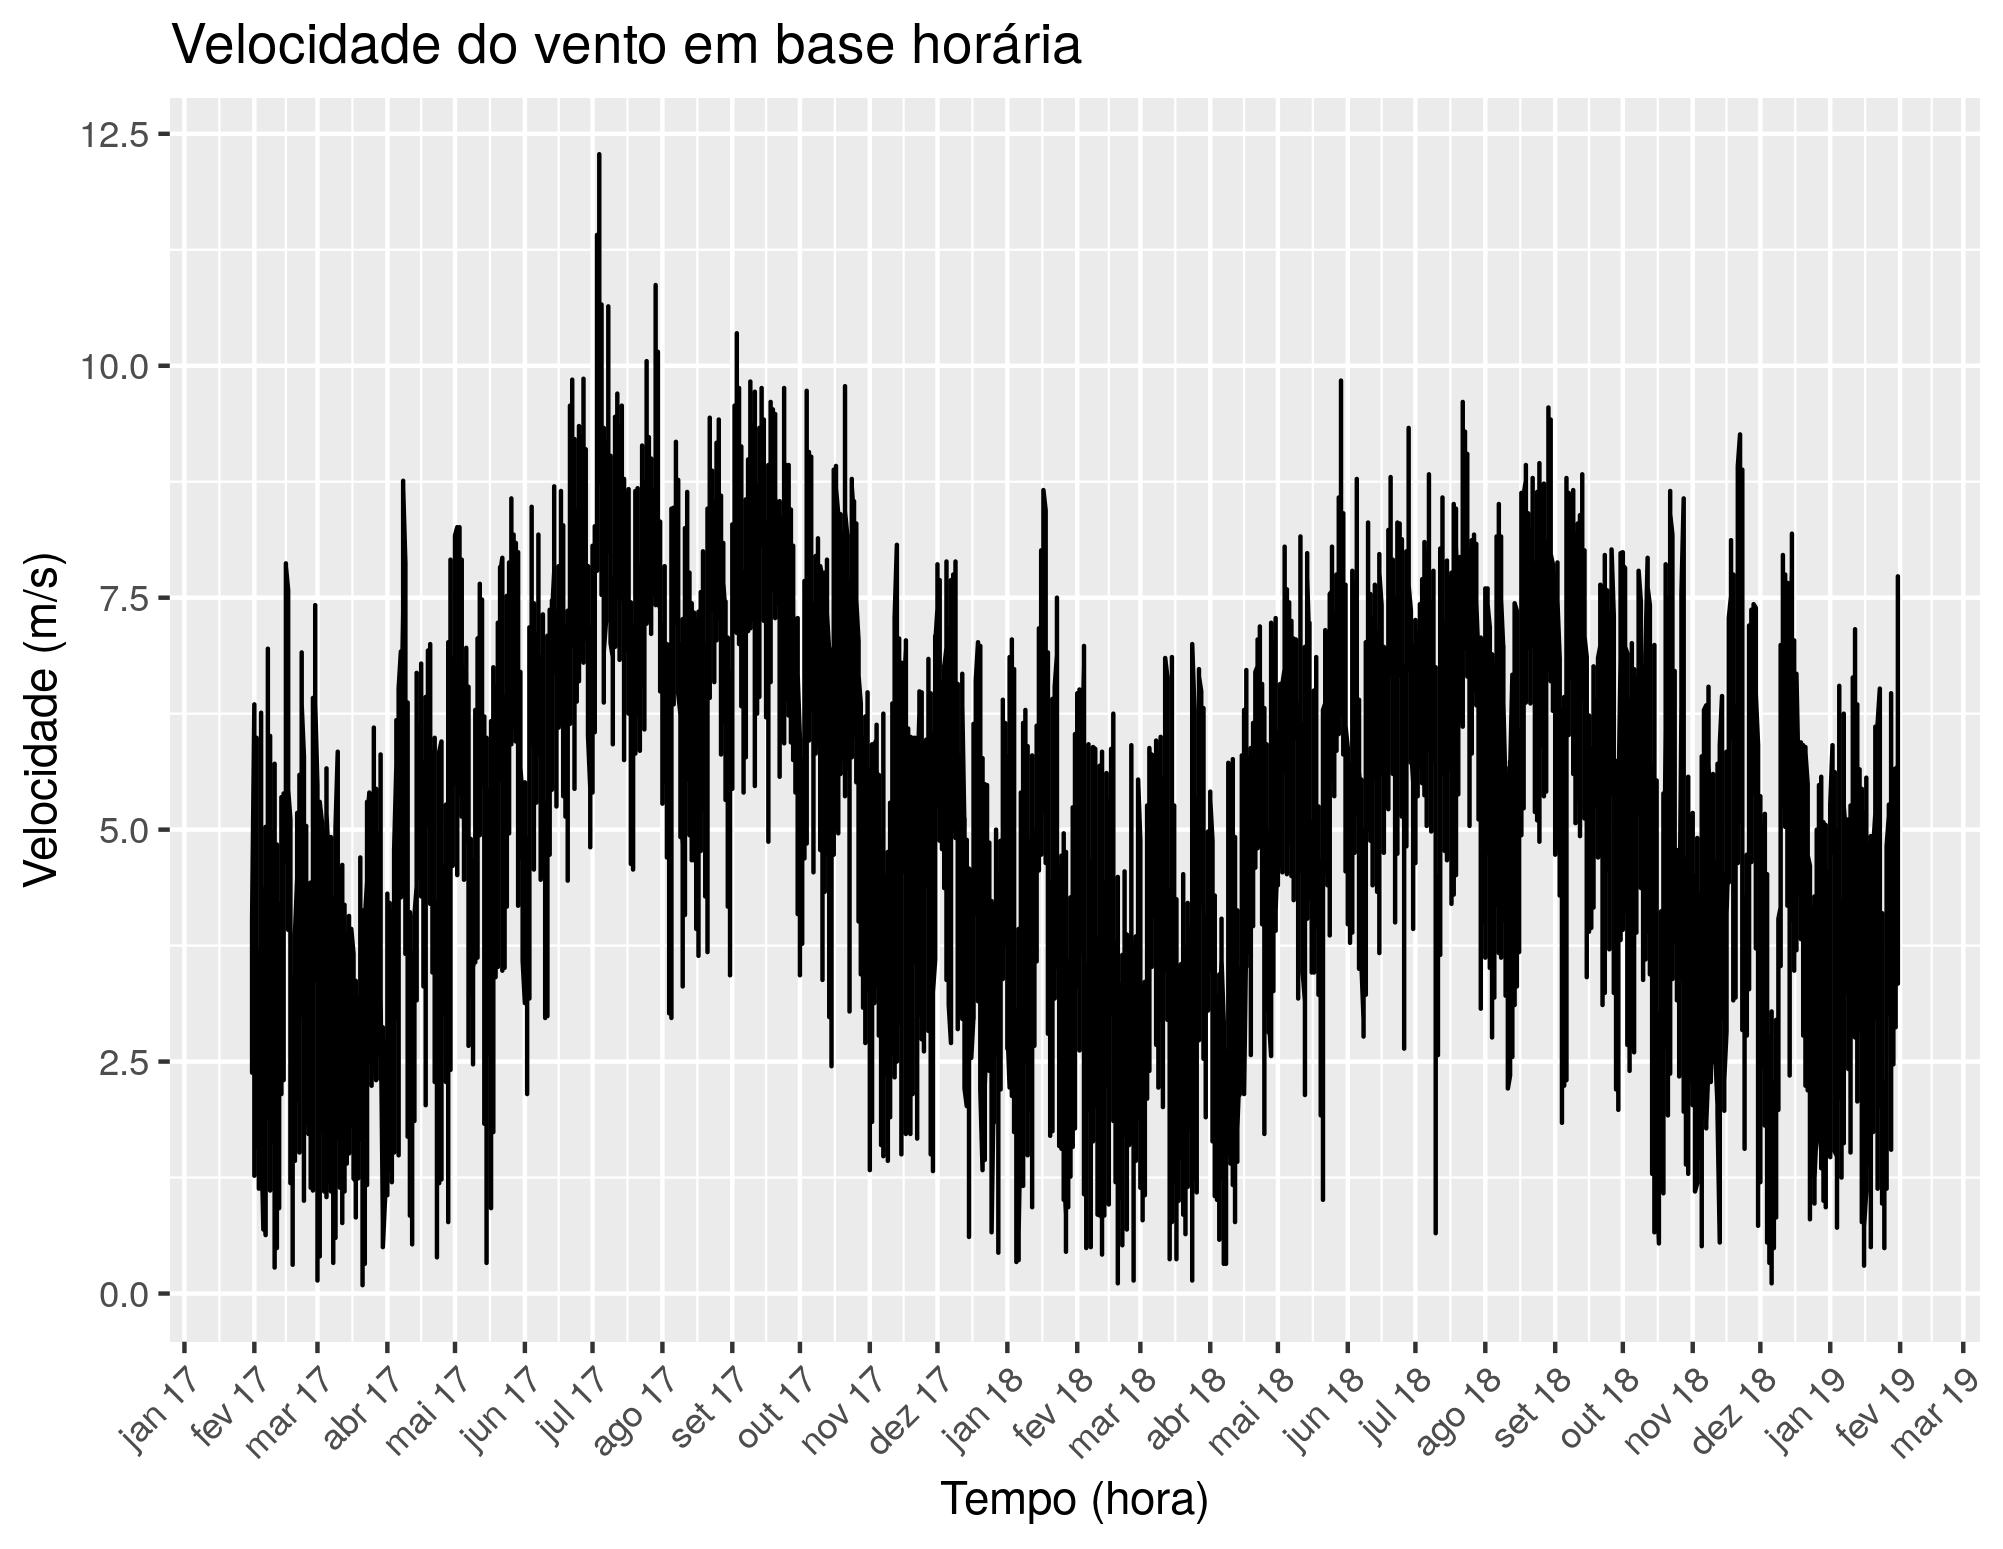
\includegraphics[width=\textwidth]{entire_series_hourly_basis}
		\caption{Últimos dois anos da série de vento}
	\end{figure}
\end{frame}

\begin{frame}
	\frametitle{Sazonalidade removida}
	\begin{figure}
		\centering
		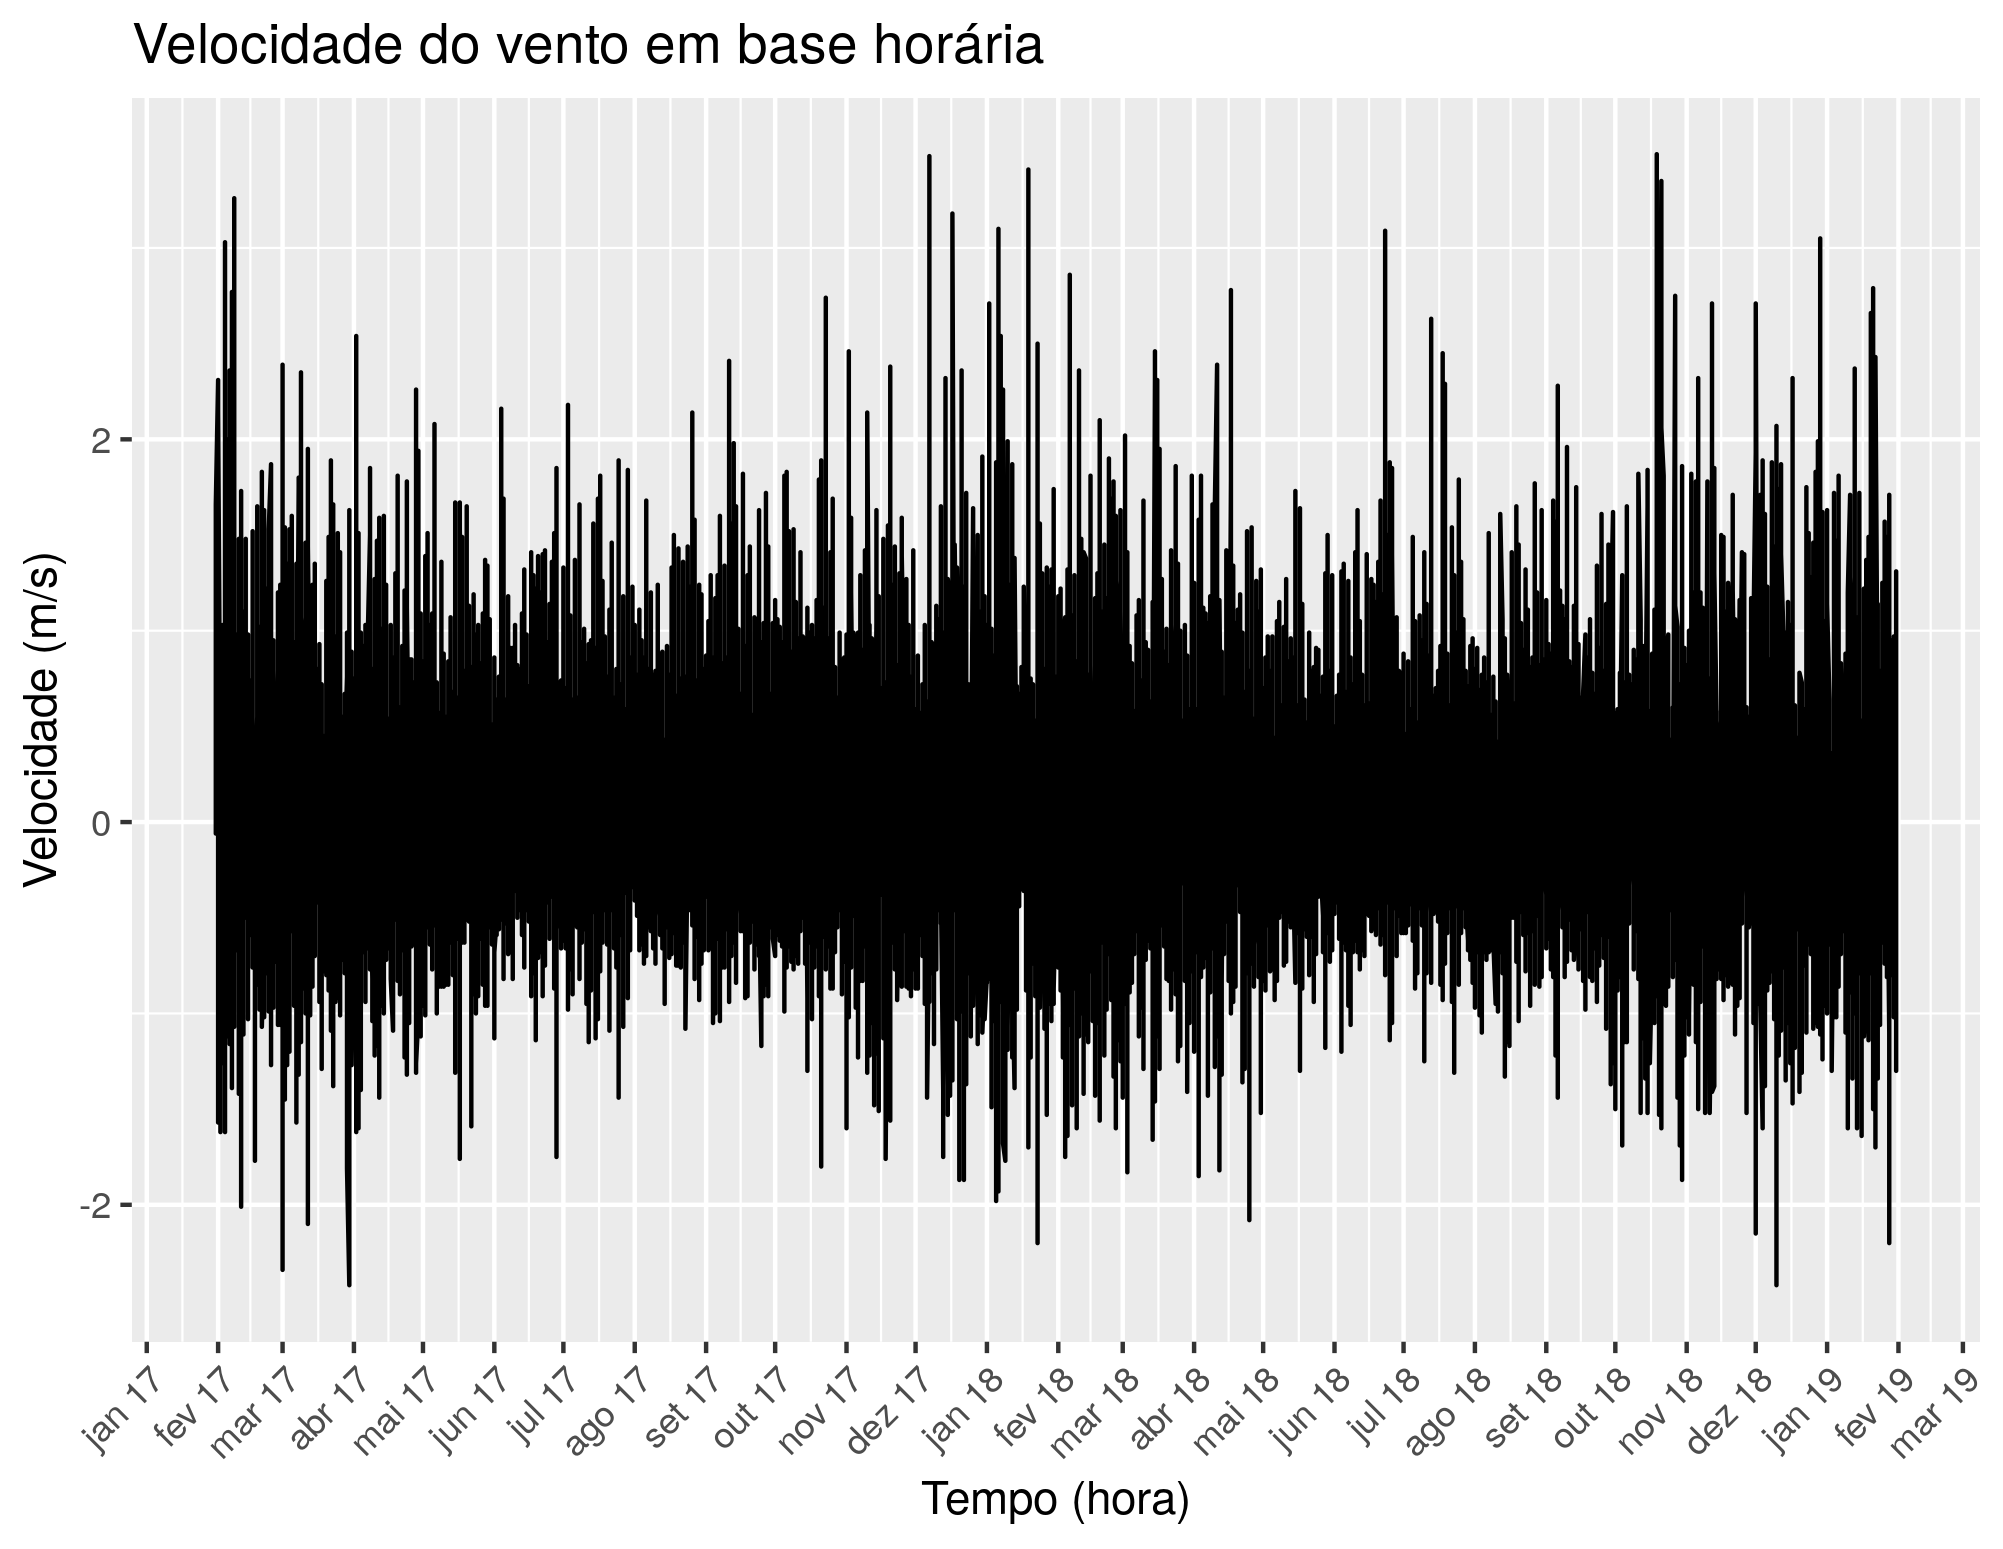
\includegraphics[width=\textwidth]{entire_series_hourly_basis_seasonless.png}
		\caption{Sazonalidade removida}
	\end{figure}
\end{frame}

\begin{frame}
	\frametitle{Sazonalidade removida por meio de uma transformação de Box-Cox}
	\begin{figure}
		\centering
		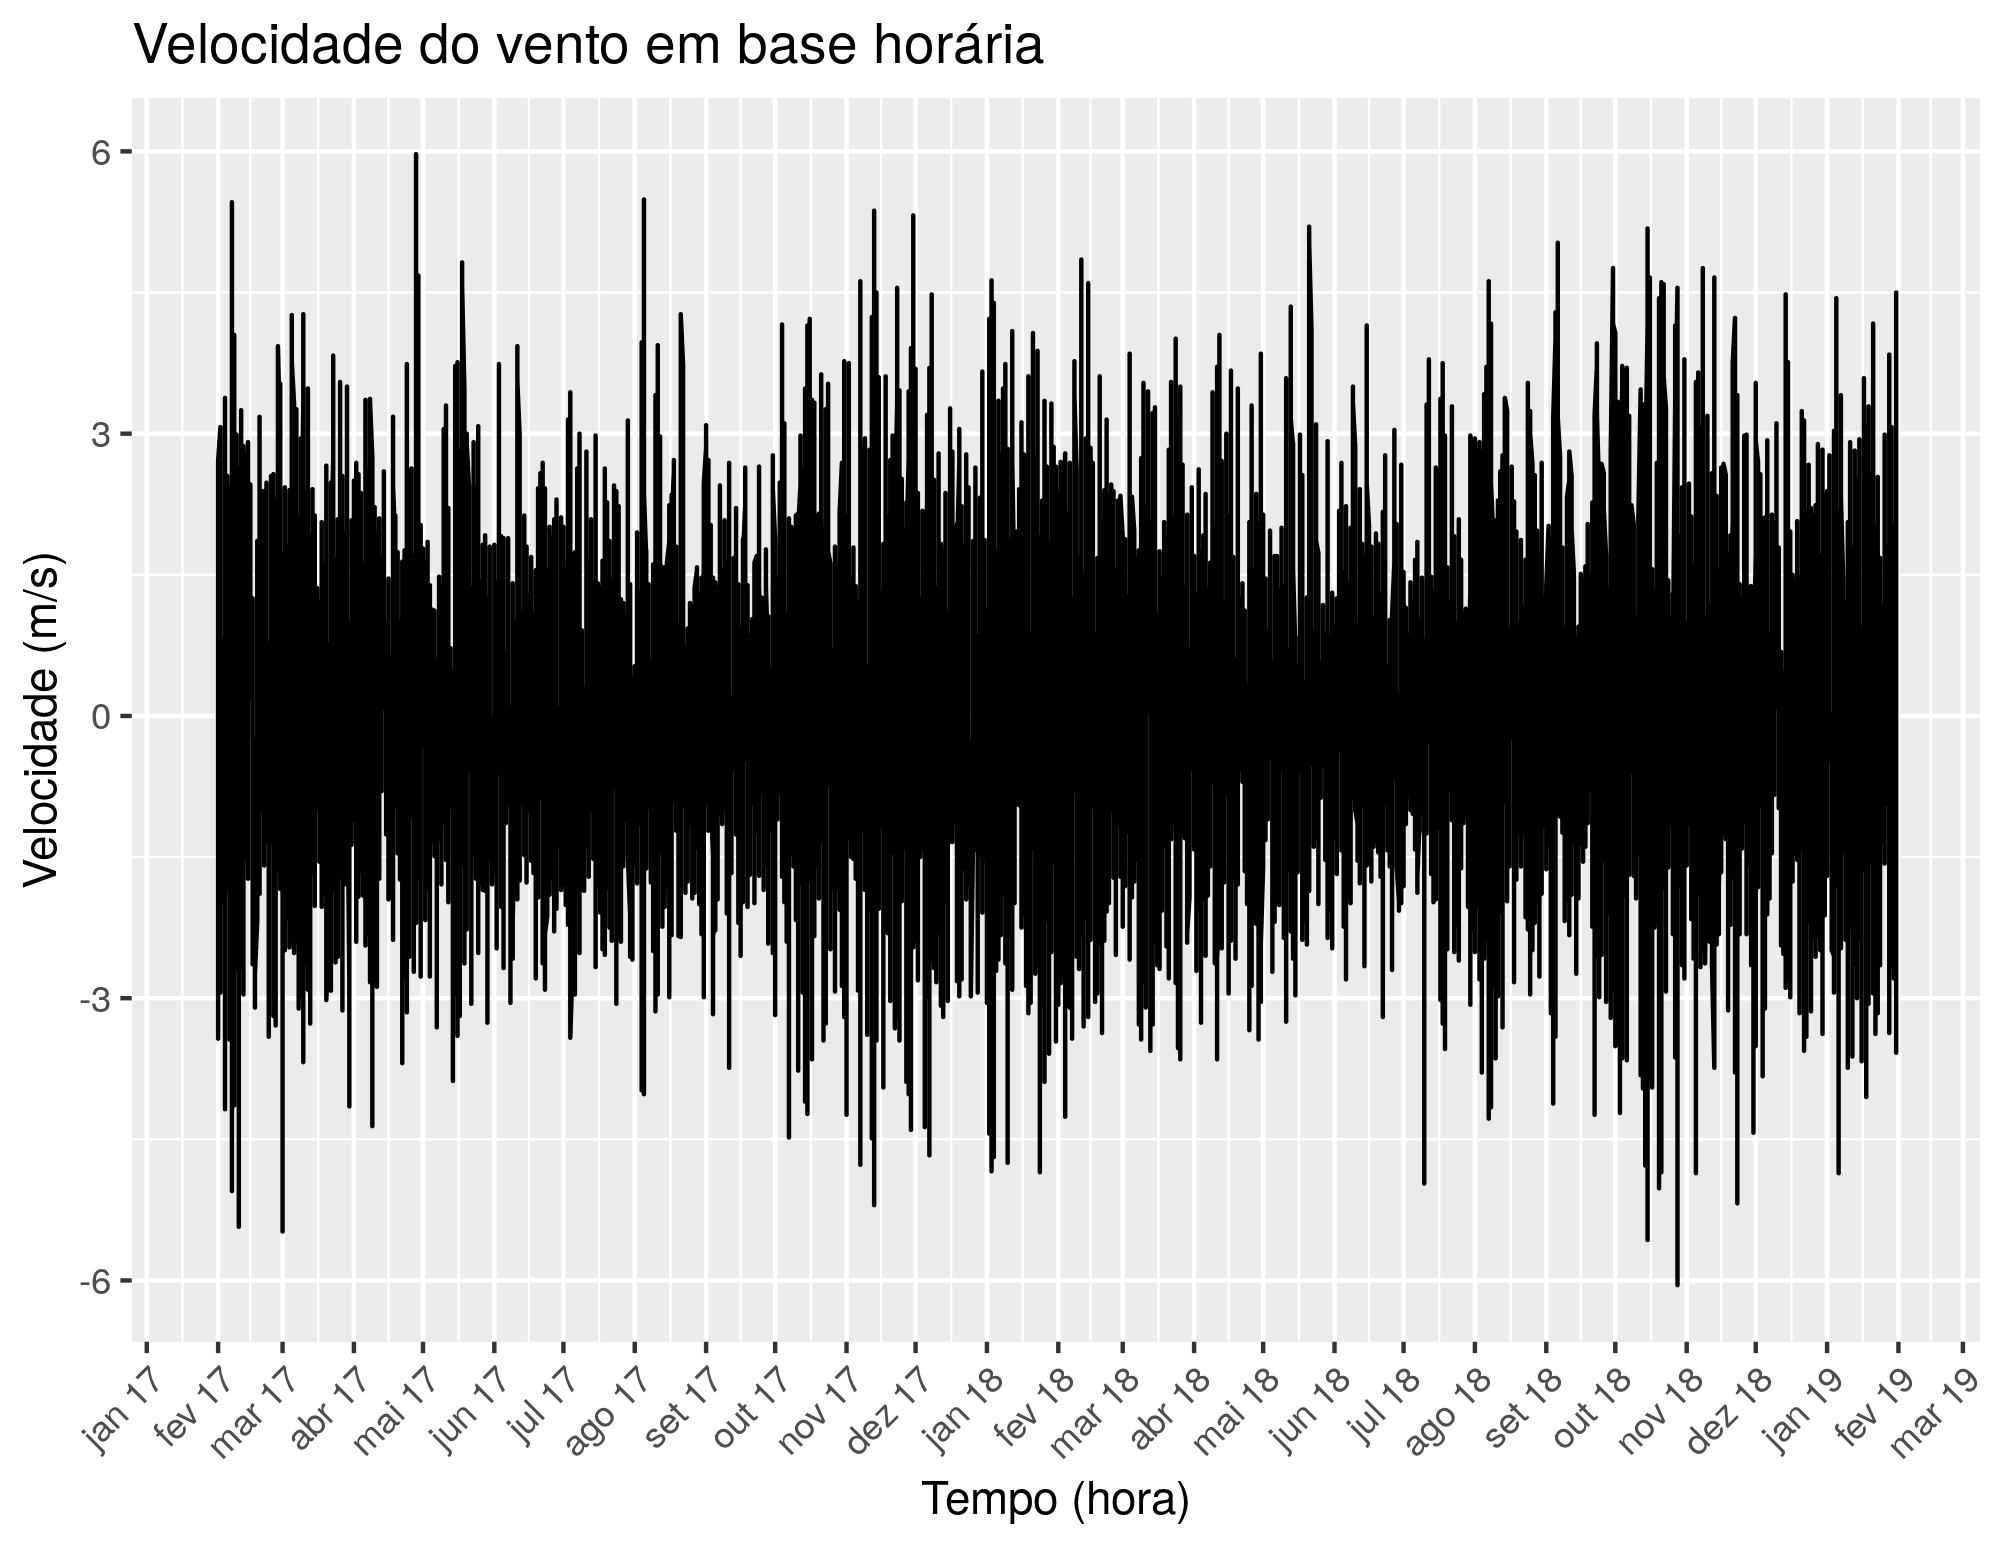
\includegraphics[width=\textwidth]{entire_series_hourly_basis_seasonless_boxcox.png}
		\caption{Sazonalidade removida por meio de uma transformação de Box-Cox}
	\end{figure}
\end{frame}

\begin{frame}
	\frametitle{Gráficos da Função de Autocorrelação (ACF) e Função de Autocorrelação Parcial (PACF)}
	\begin{figure}
		\centering
		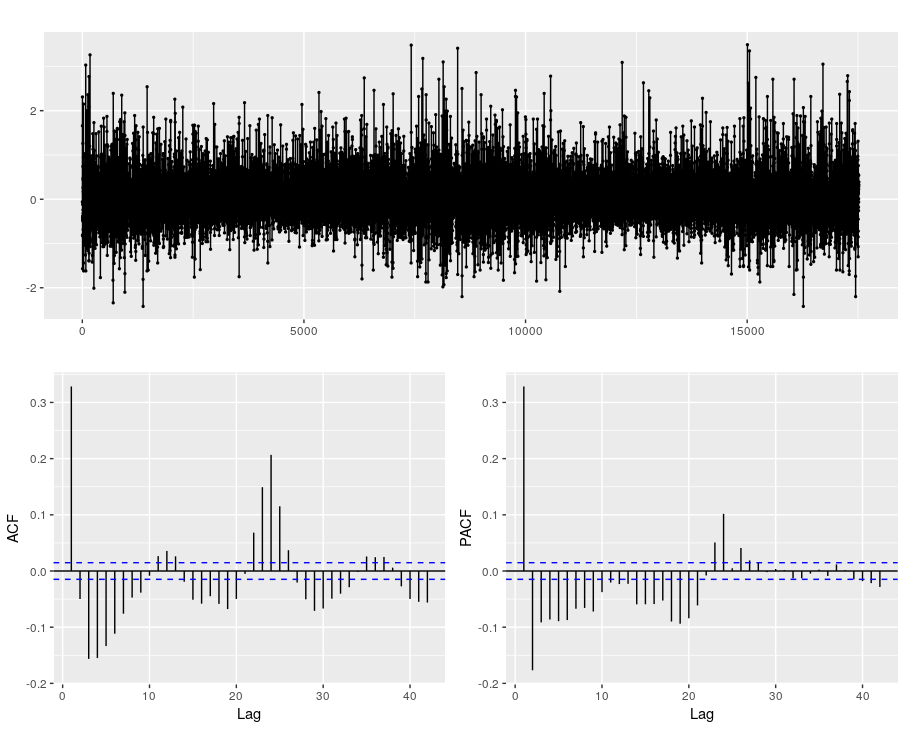
\includegraphics[width=\textwidth]{long_memory.png}
		\caption{Gráficos da Função de Autocorrelação (ACF) e Função de Autocorrelação Parcial (PACF)}
	\end{figure}
\end{frame}

\begin{frame}
	\frametitle{Gráficos da Função de Autocorrelação (ACF) e Função de Autocorrelação Parcial (PACF)}
	\begin{figure}
		\centering
		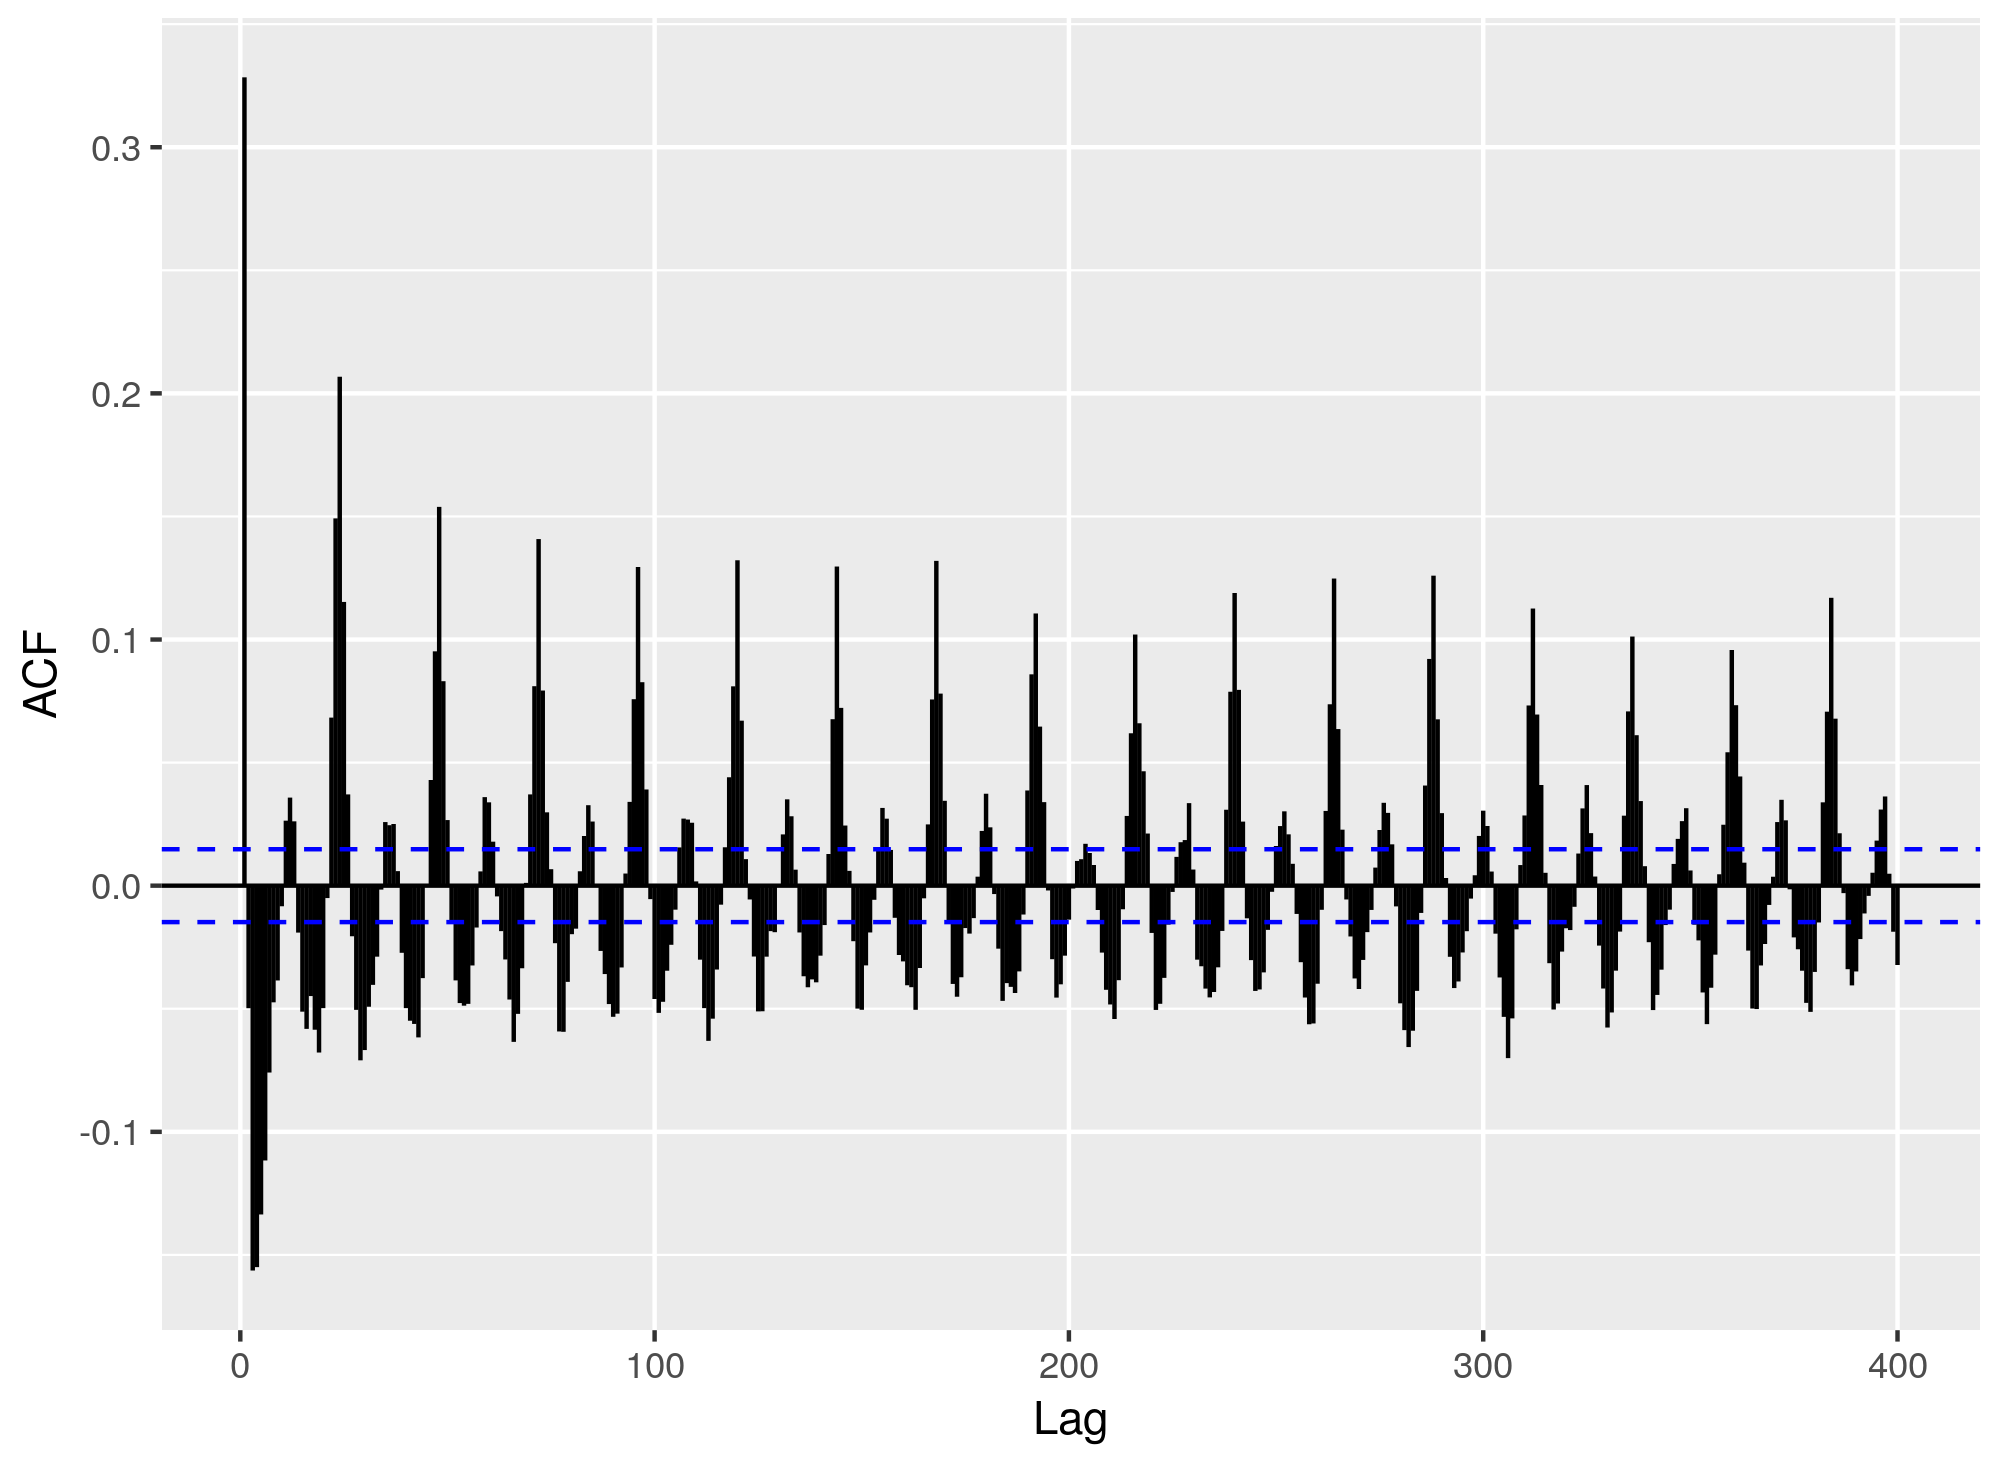
\includegraphics[width=\textwidth]{long_memory_lagmax.png}
		\caption{Gráficos da Função de Autocorrelação (ACF) e Função de Autocorrelação Parcial (PACF)}
	\end{figure}
\end{frame}

\begin{frame}
	\frametitle{Modelo LSTM aplicado a série. Velocidade no eixo y. Tempo em horas no eixo x.}
	\begin{figure}
		\centering
		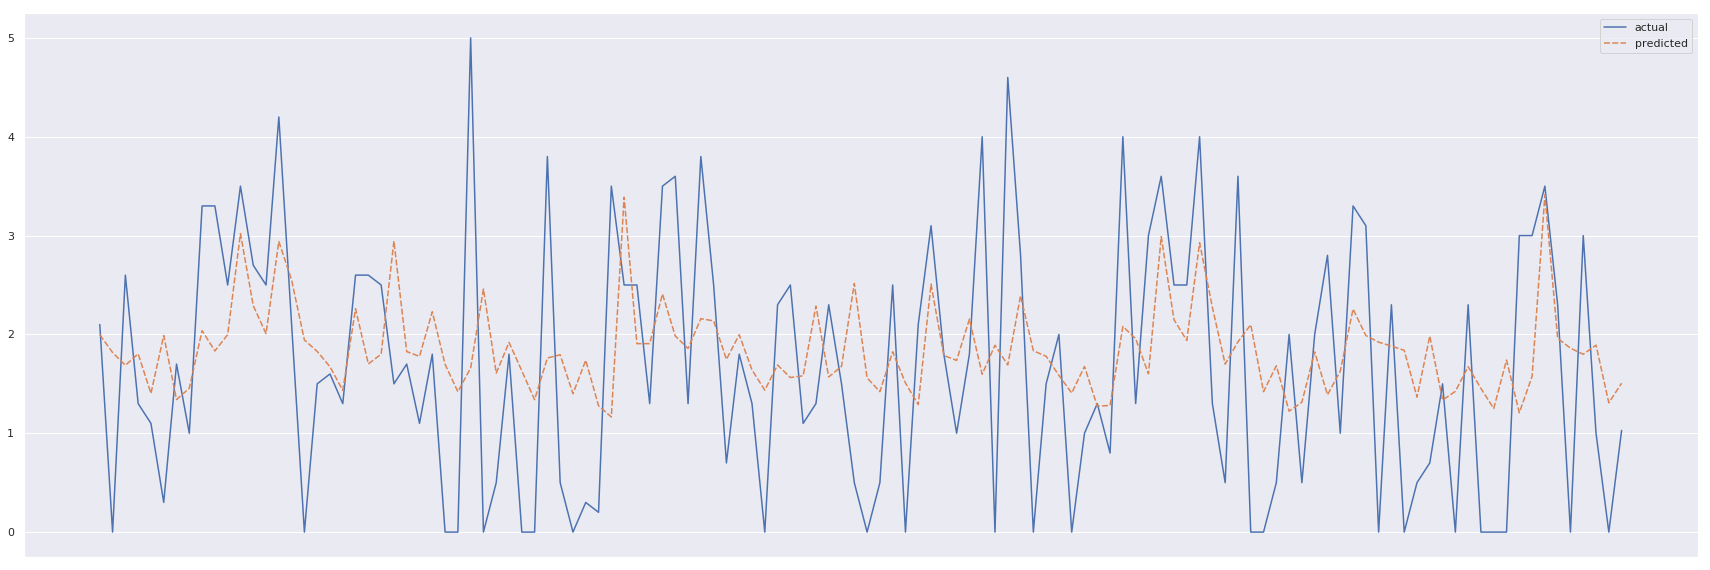
\includegraphics[width=\textwidth]{lstm.png}
		\caption{Modelo LSTM aplicado a série. Velocidade no eixo y. Tempo em horas no eixo x.}
	\end{figure}
\end{frame}

\begin{frame}
	\frametitle{3 útimas semanas de dados da série. Antes da diferenciação (superior) e após (inferior).}
	\begin{figure}
		\centering
		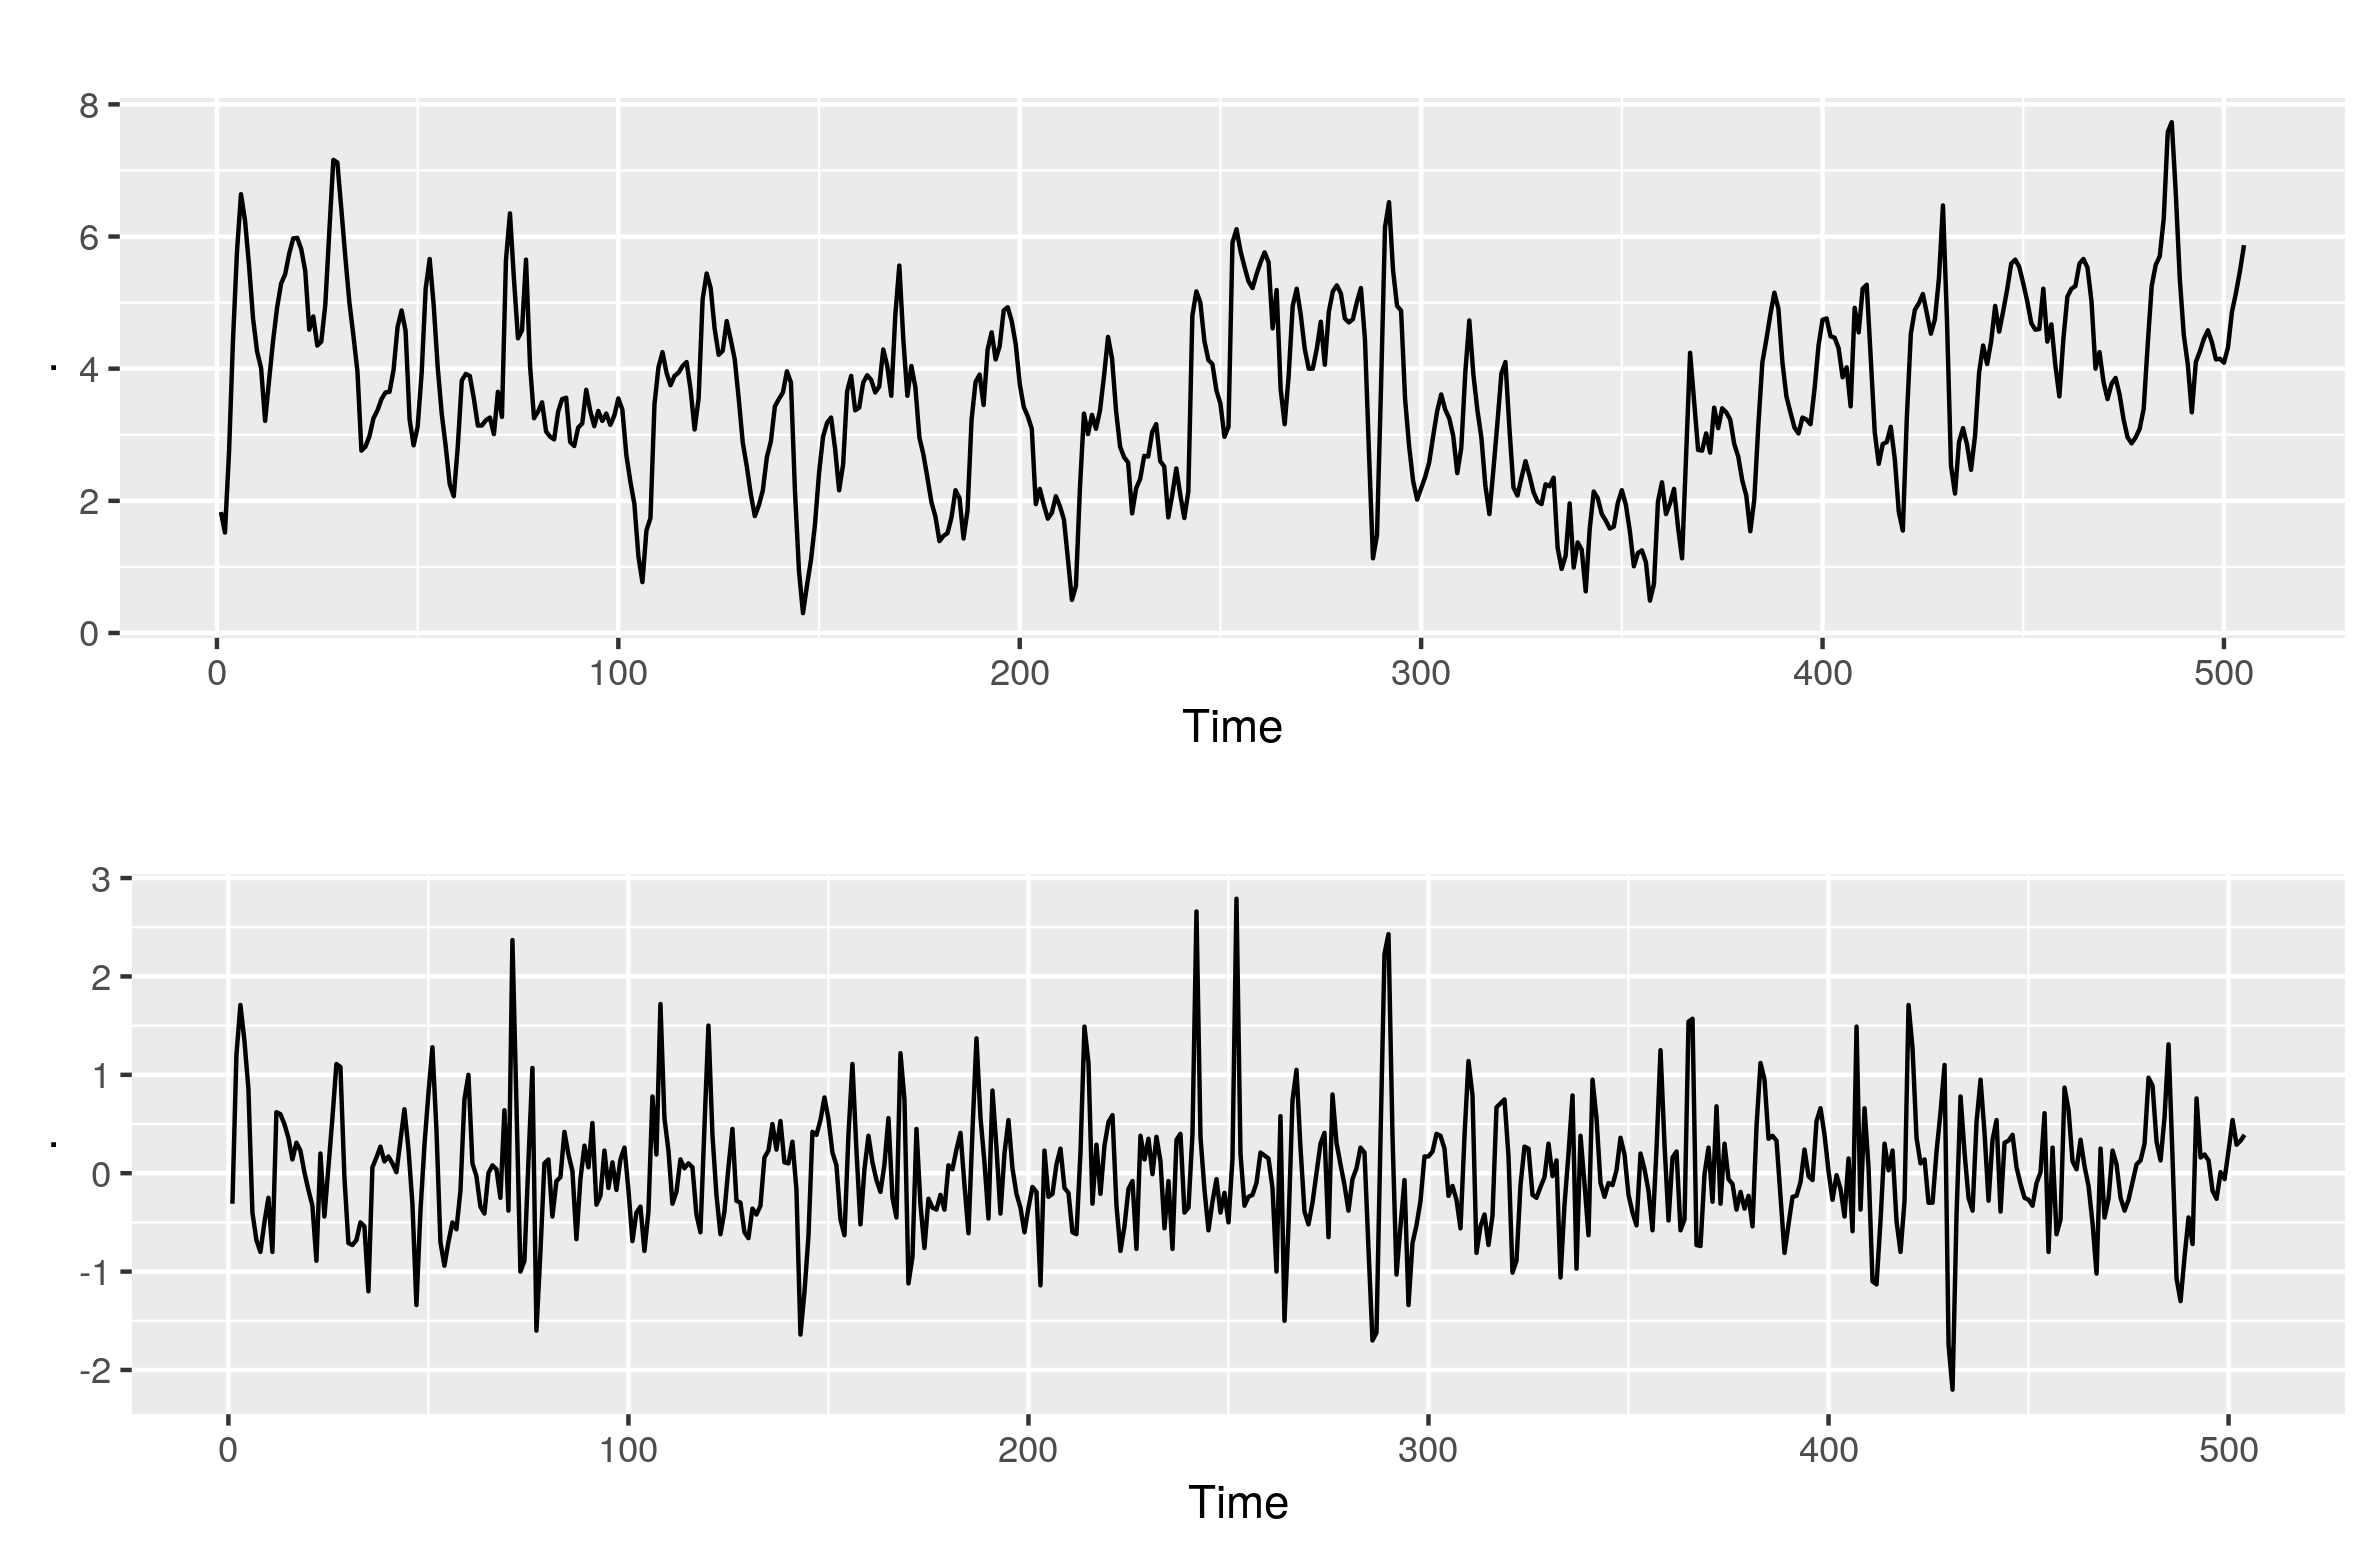
\includegraphics[width=\textwidth]{last3weeks.png}
		\caption{3 útimas semanas de dados da série. Antes da diferenciação (superior) e após (inferior).}
	\end{figure}
\end{frame}

\begin{frame}
	\frametitle{Gráficos da Função de Autocorrelação e Autocorrelação Parical para 2 semanas de dados da série.}
	\begin{figure}
		\centering
		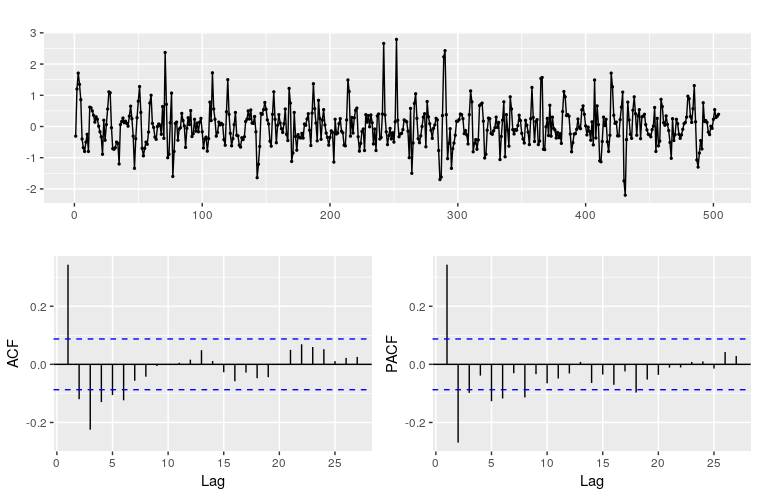
\includegraphics[width=\textwidth]{last3weeks_acf.png}
		\caption{Gráficos da Função de Autocorrelação e Autocorrelação Parical para 2 semanas de dados da série.}
	\end{figure}
\end{frame}

\begin{frame}
	\frametitle{Chapada}
	\begin{figure}
		\centering
		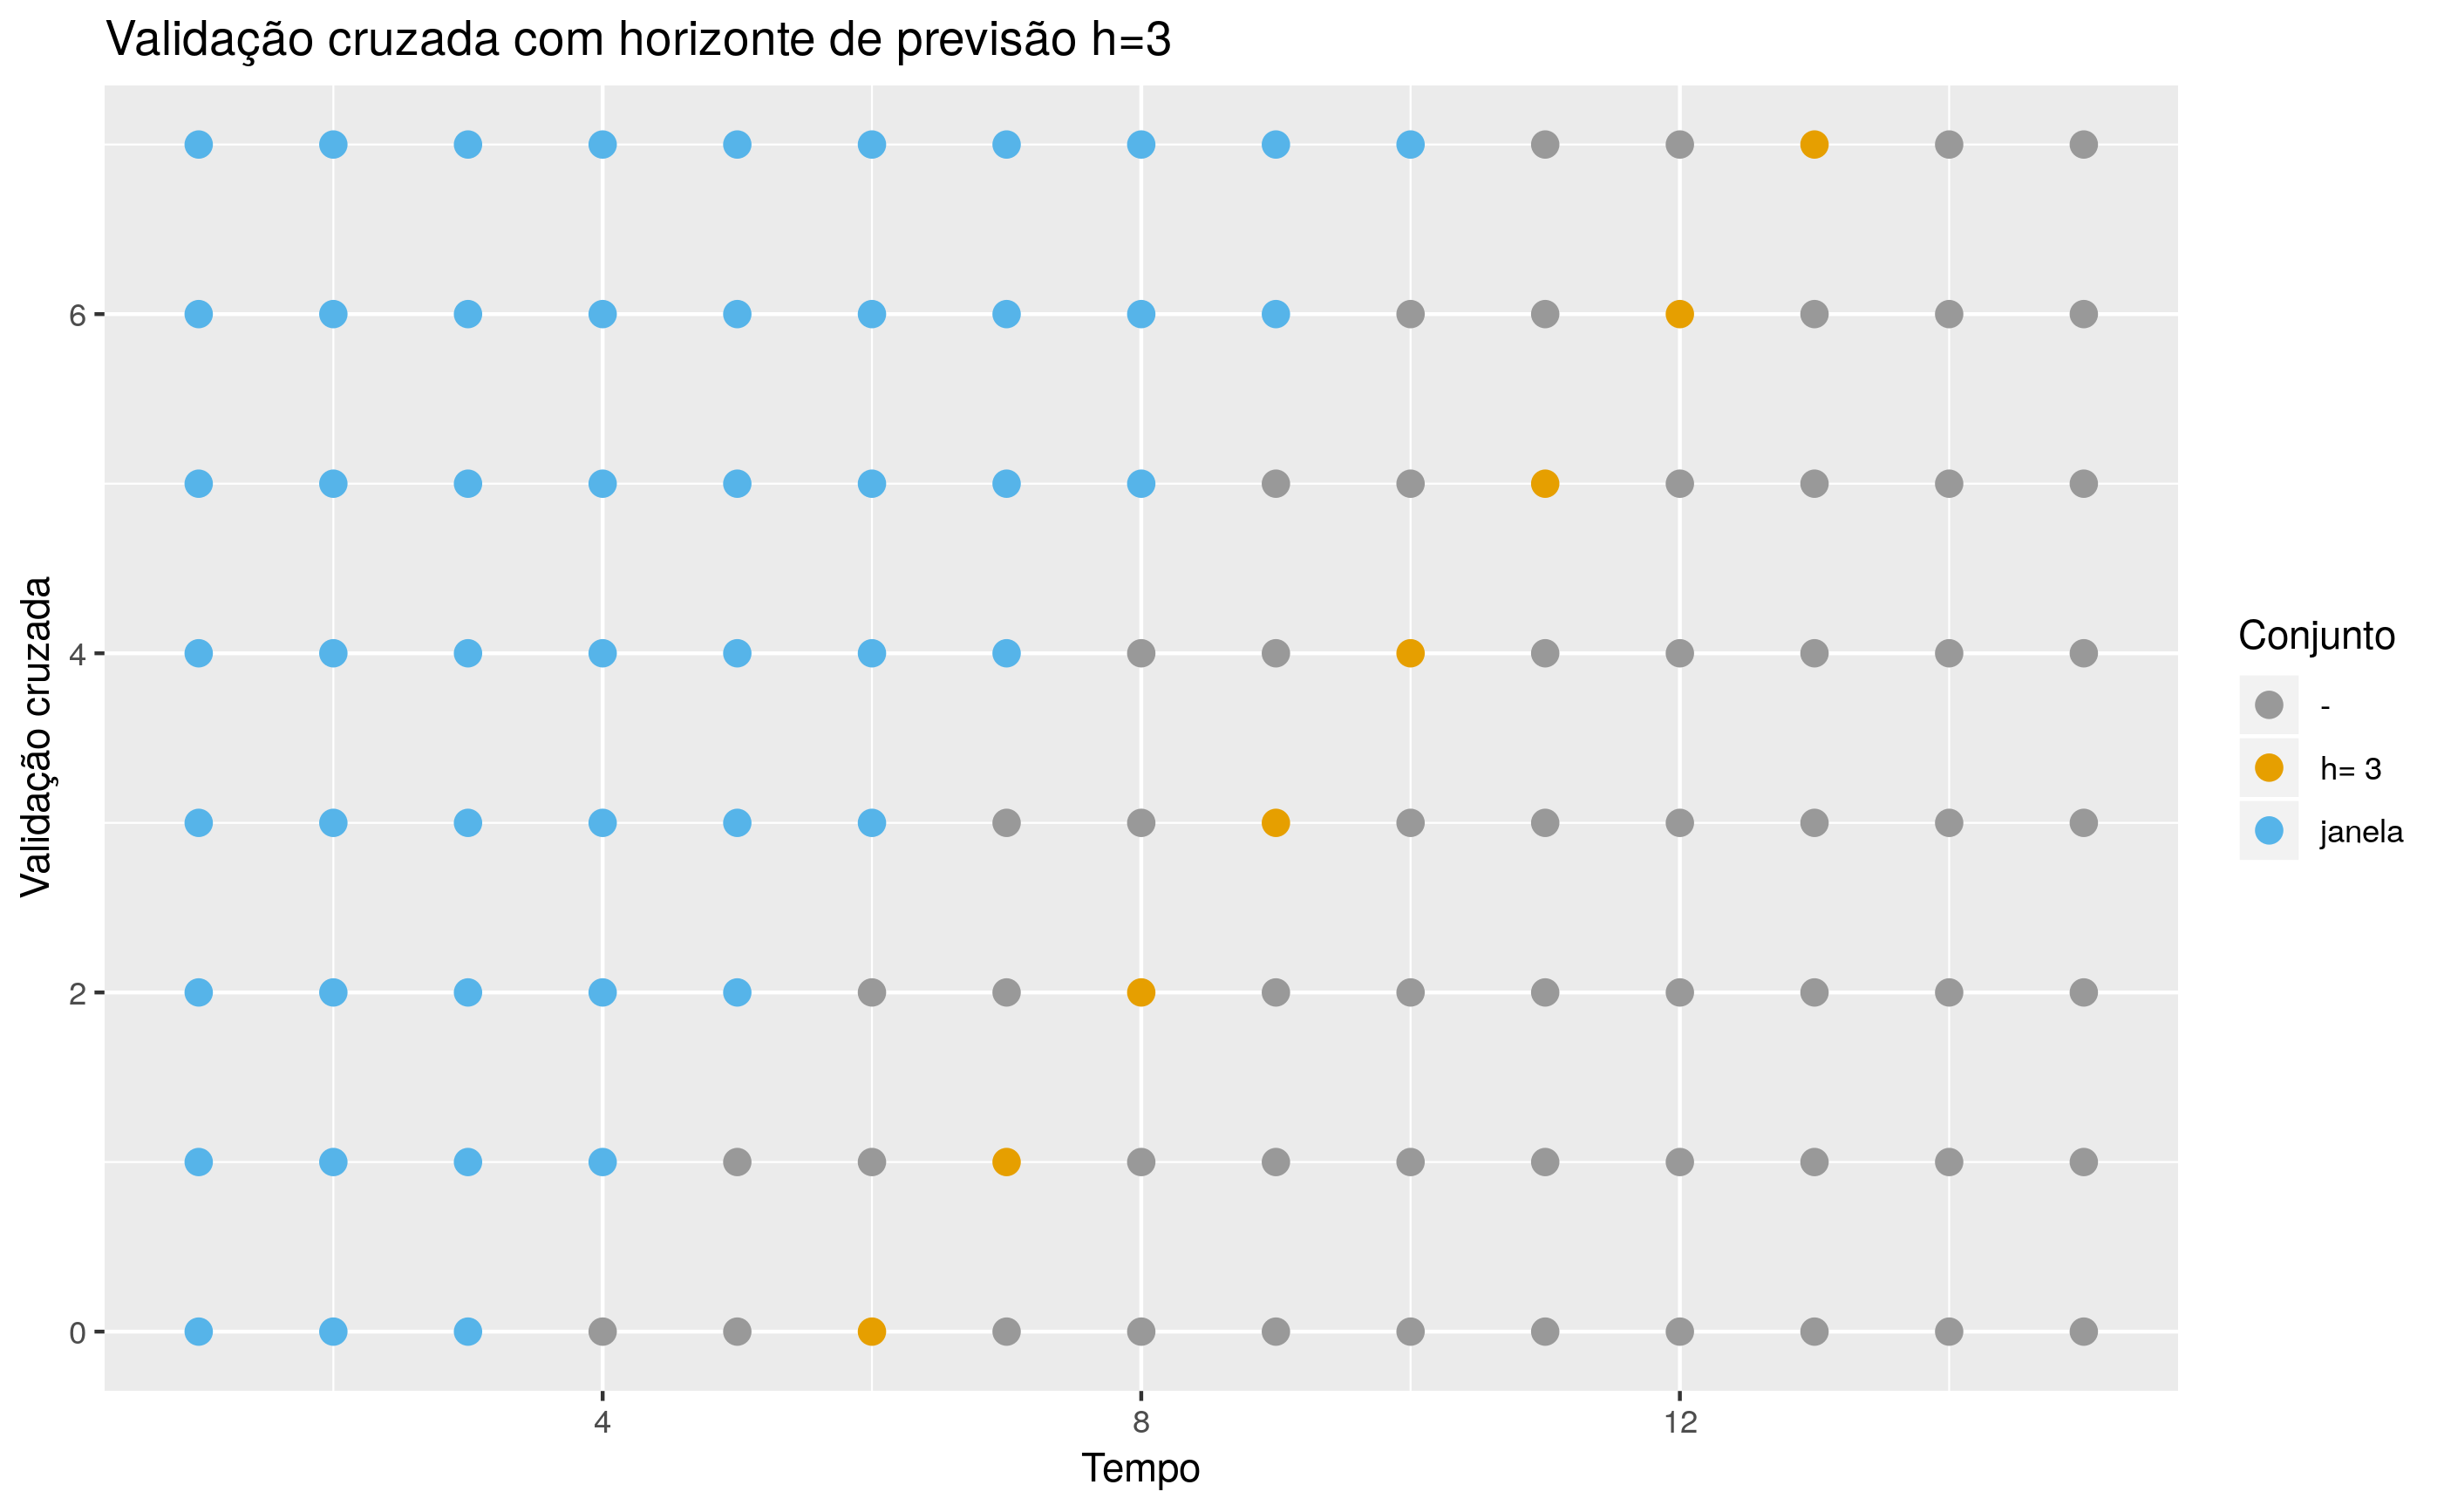
\includegraphics[width=\textwidth]{crossh3}
		\caption{Chapada}
	\end{figure}
\end{frame}

\begin{frame}
	\frametitle{Condições de regime estacionário e invertibilidade para um modelo ARIMA(6,1,0).}
	\begin{figure}
		\centering
		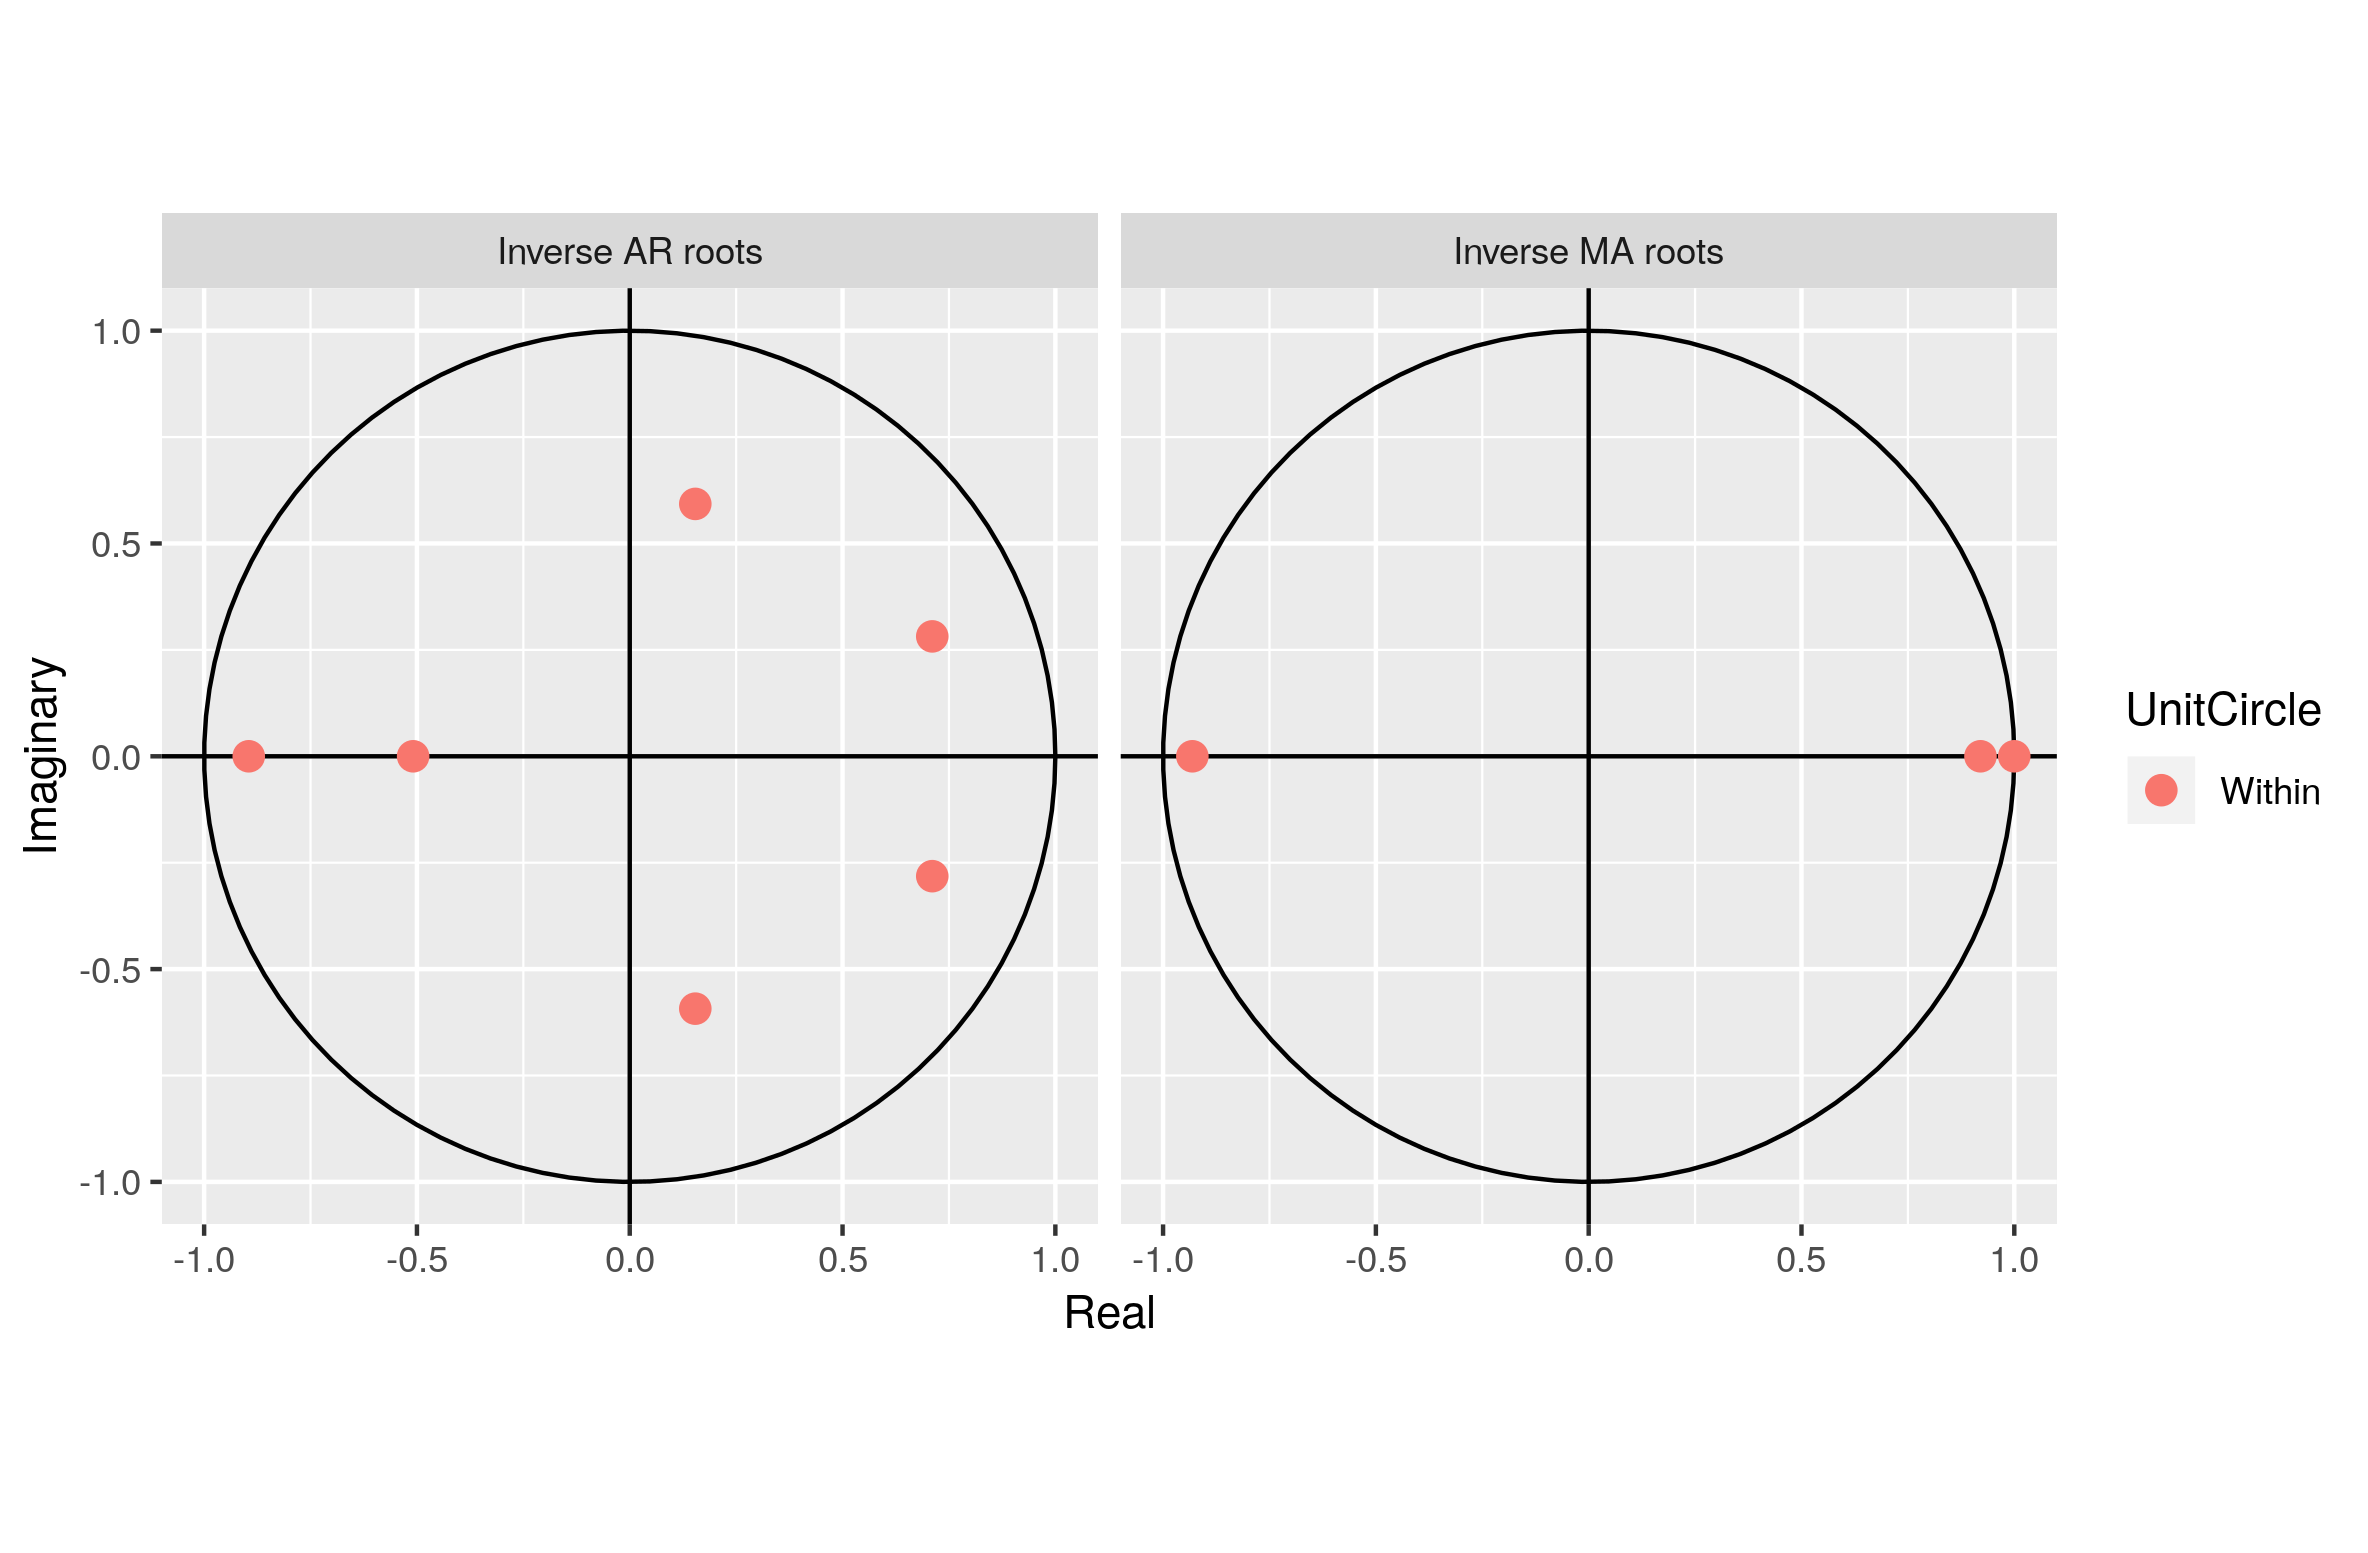
\includegraphics[width=\textwidth]{conds}
		\caption{Condições de regime estacionário e invertibilidade para um modelo ARIMA(6,1,0).}
	\end{figure}
\end{frame}

\begin{frame}
	\frametitle{Condições de regime estacionário e invertibilidade para um modelo ARIMA(6,1,0).}
	\begin{figure}
		\centering
		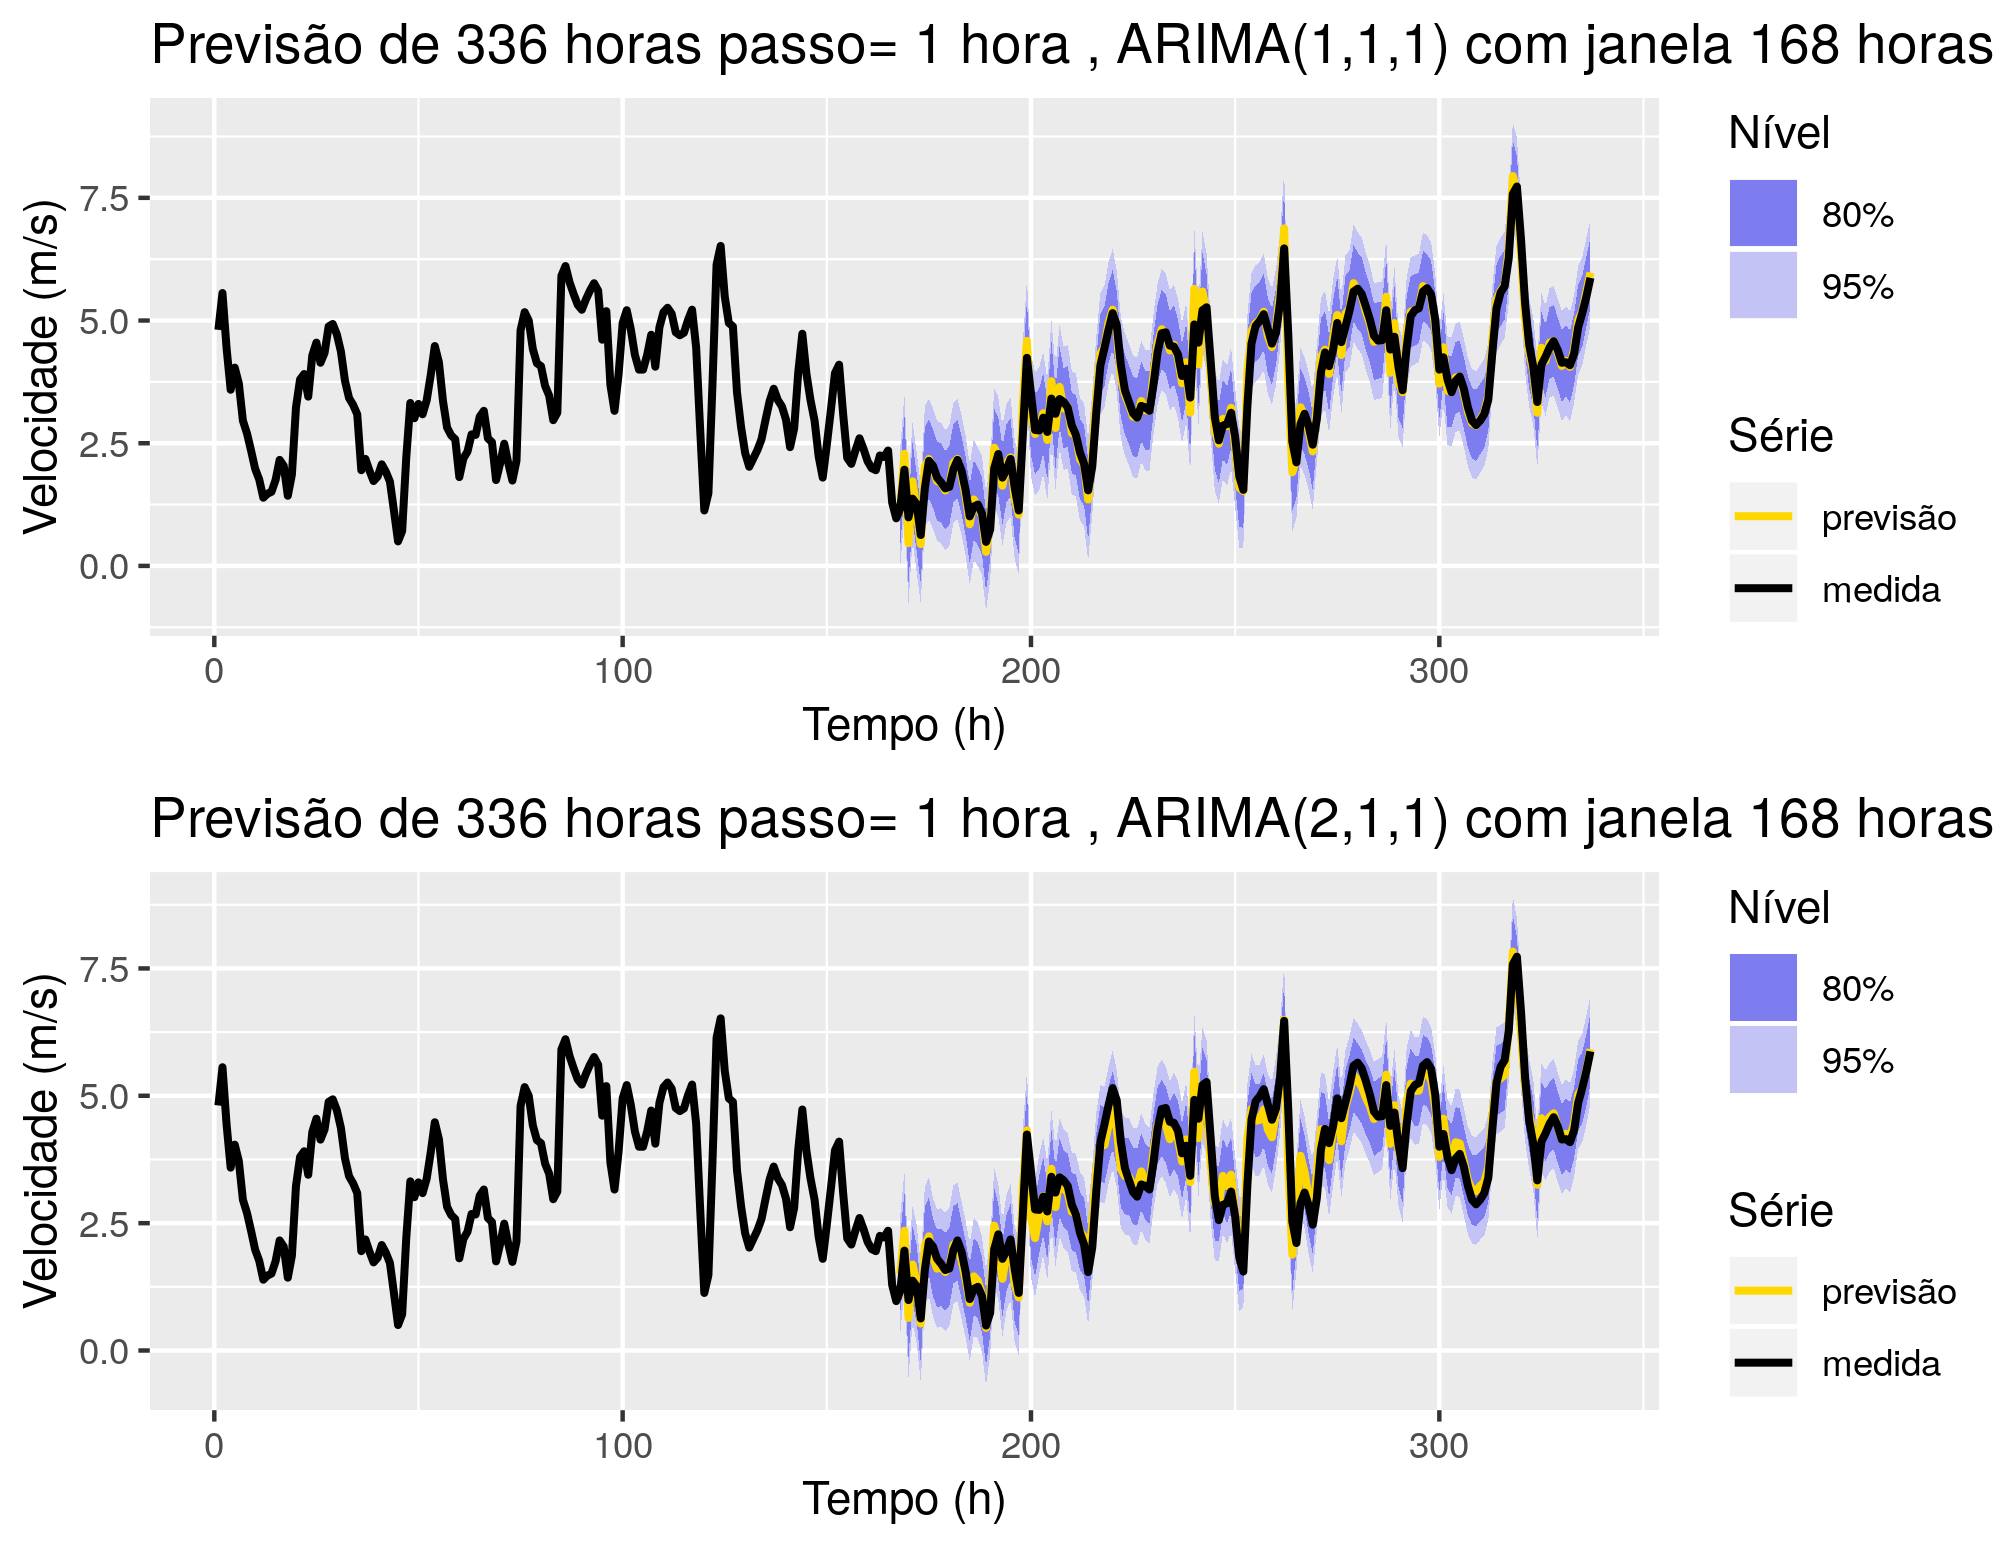
\includegraphics[width=\textwidth]{arima12}
		\caption{Condições de regime estacionário e invertibilidade para um modelo ARIMA(6,1,0).}
	\end{figure}
\end{frame}

\begin{frame}
	\frametitle{Condições de regime estacionário e invertibilidade para um modelo ARIMA(6,1,0).}
	\begin{figure}
		\centering
		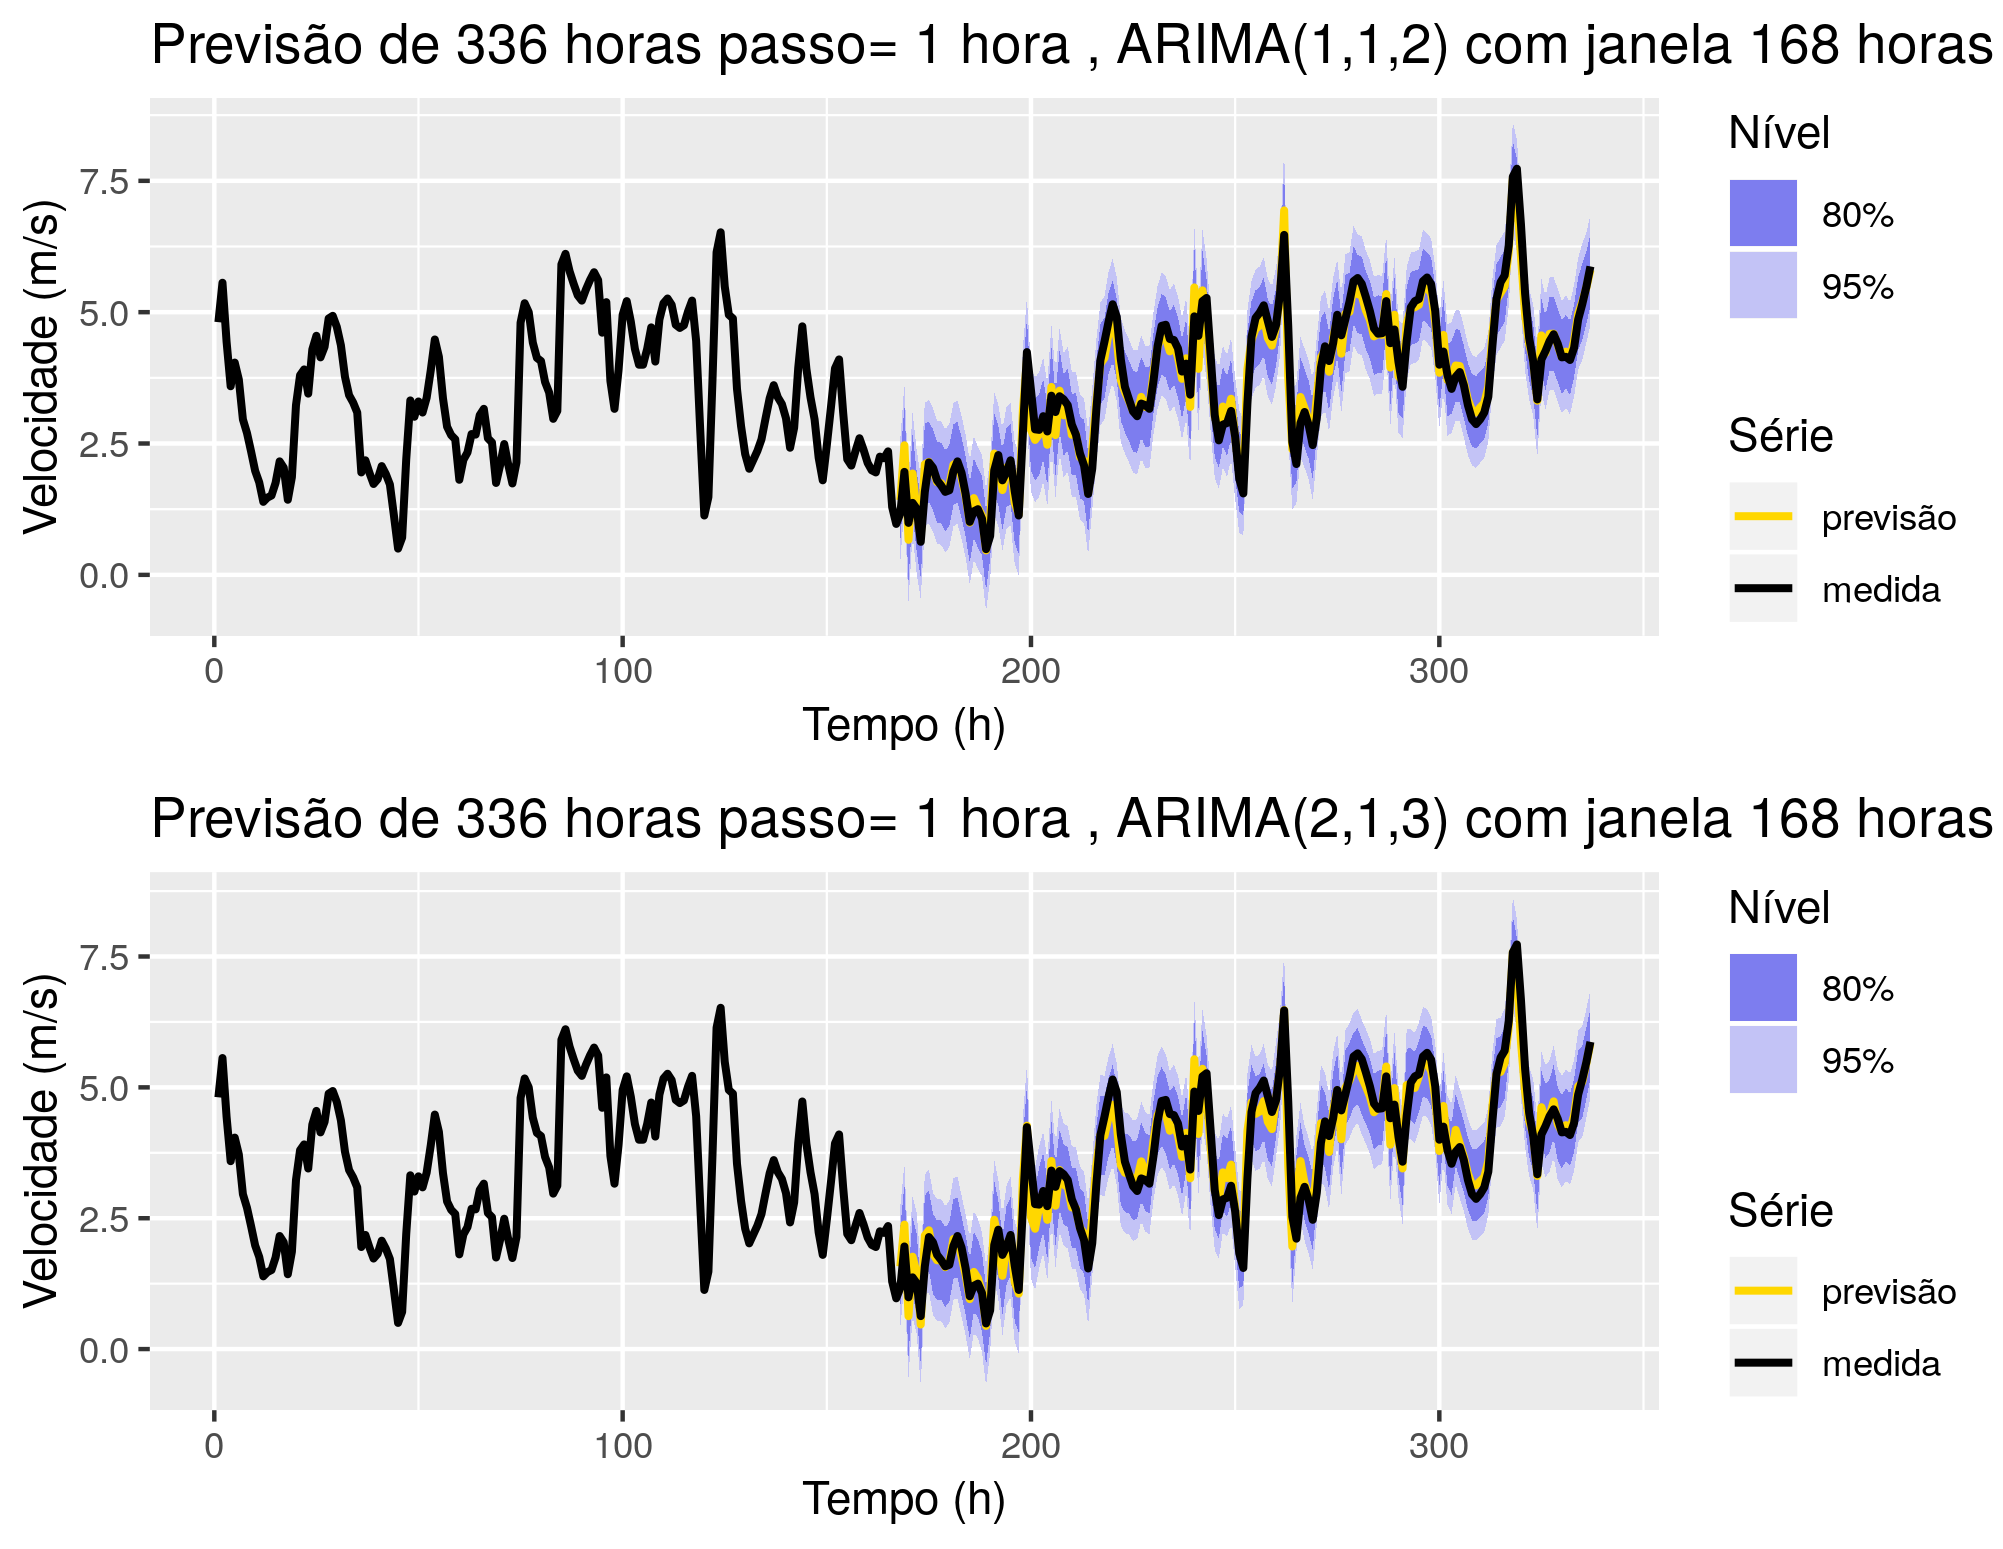
\includegraphics[width=\textwidth]{arima34}
		\caption{Condições de regime estacionário e invertibilidade para um modelo ARIMA(6,1,0).}
	\end{figure}
\end{frame}

\begin{frame}
	\frametitle{Evolução dos parâmetros p e q de um modelo ARIMA ao longo do tempo.}
	\begin{figure}
		\centering
		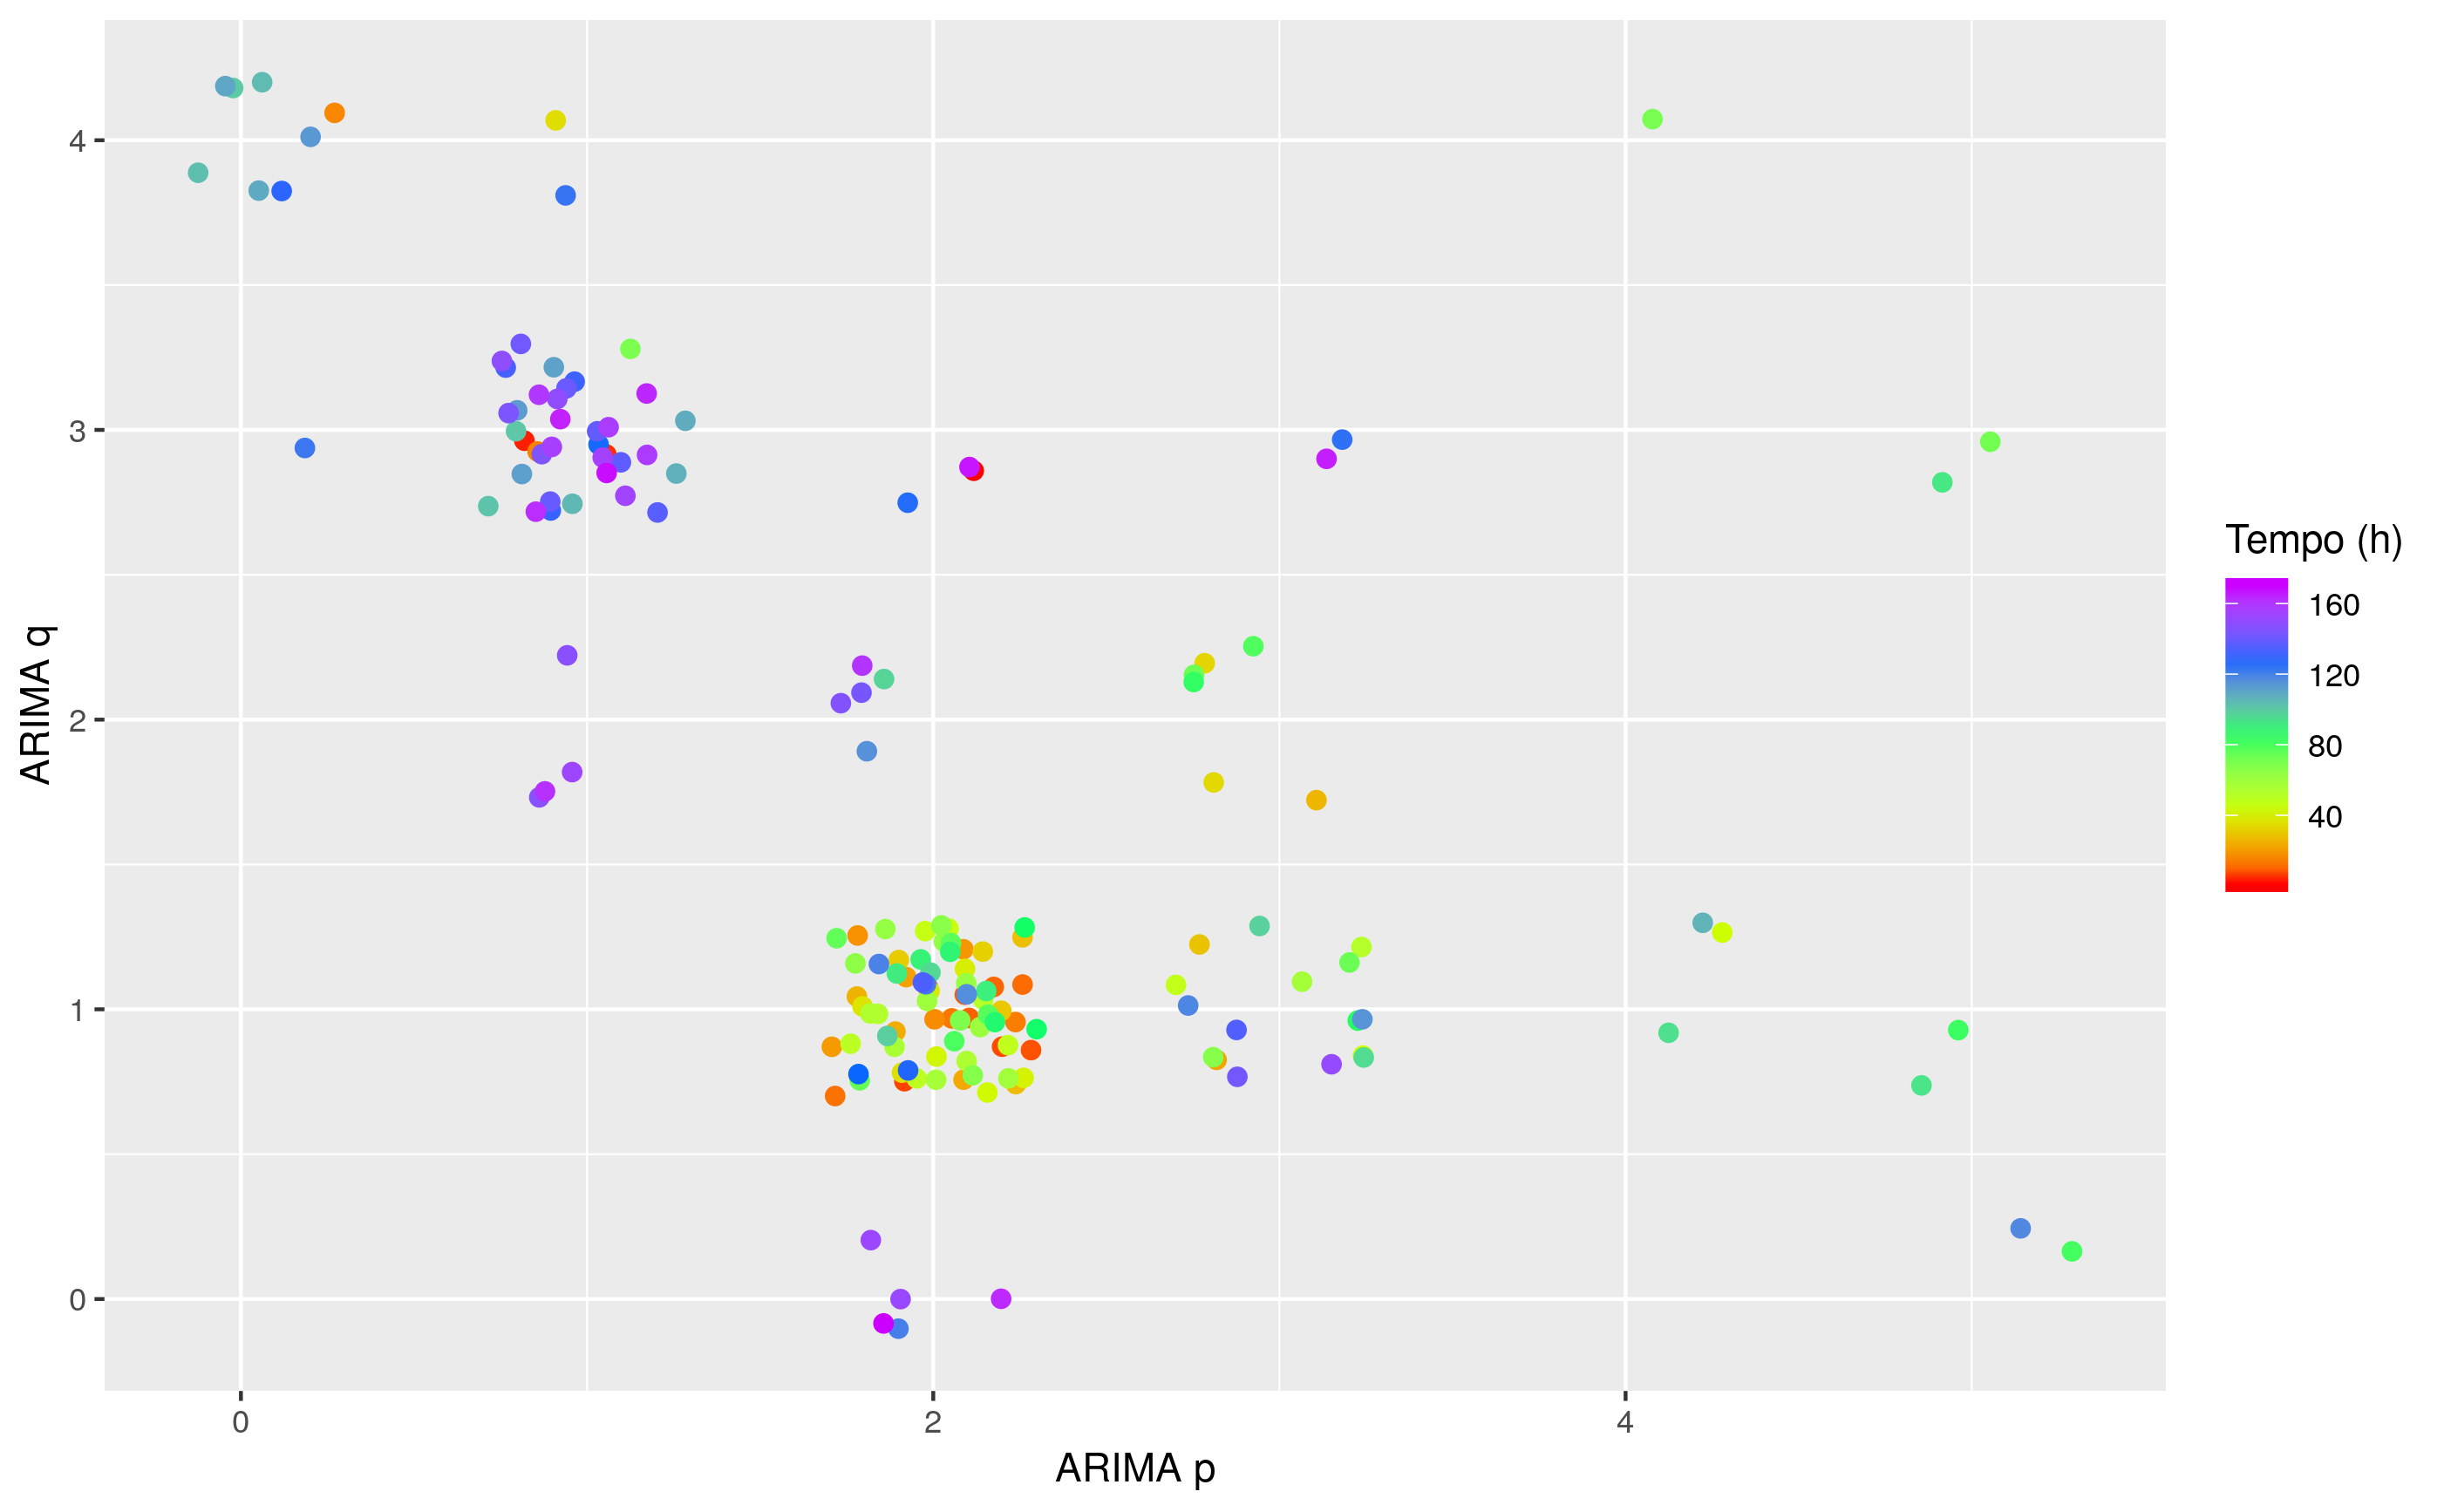
\includegraphics[width=\textwidth]{var_arima}
		\caption{Evolução dos parâmetros p e q de um modelo ARIMA ao longo do tempo.}
	\end{figure}
\end{frame}

\begin{frame}
	\frametitle{Evolução dos parâmetros p e q de um modelo ARIMA ao longo do tempo.}
	\begin{figure}
		\centering
		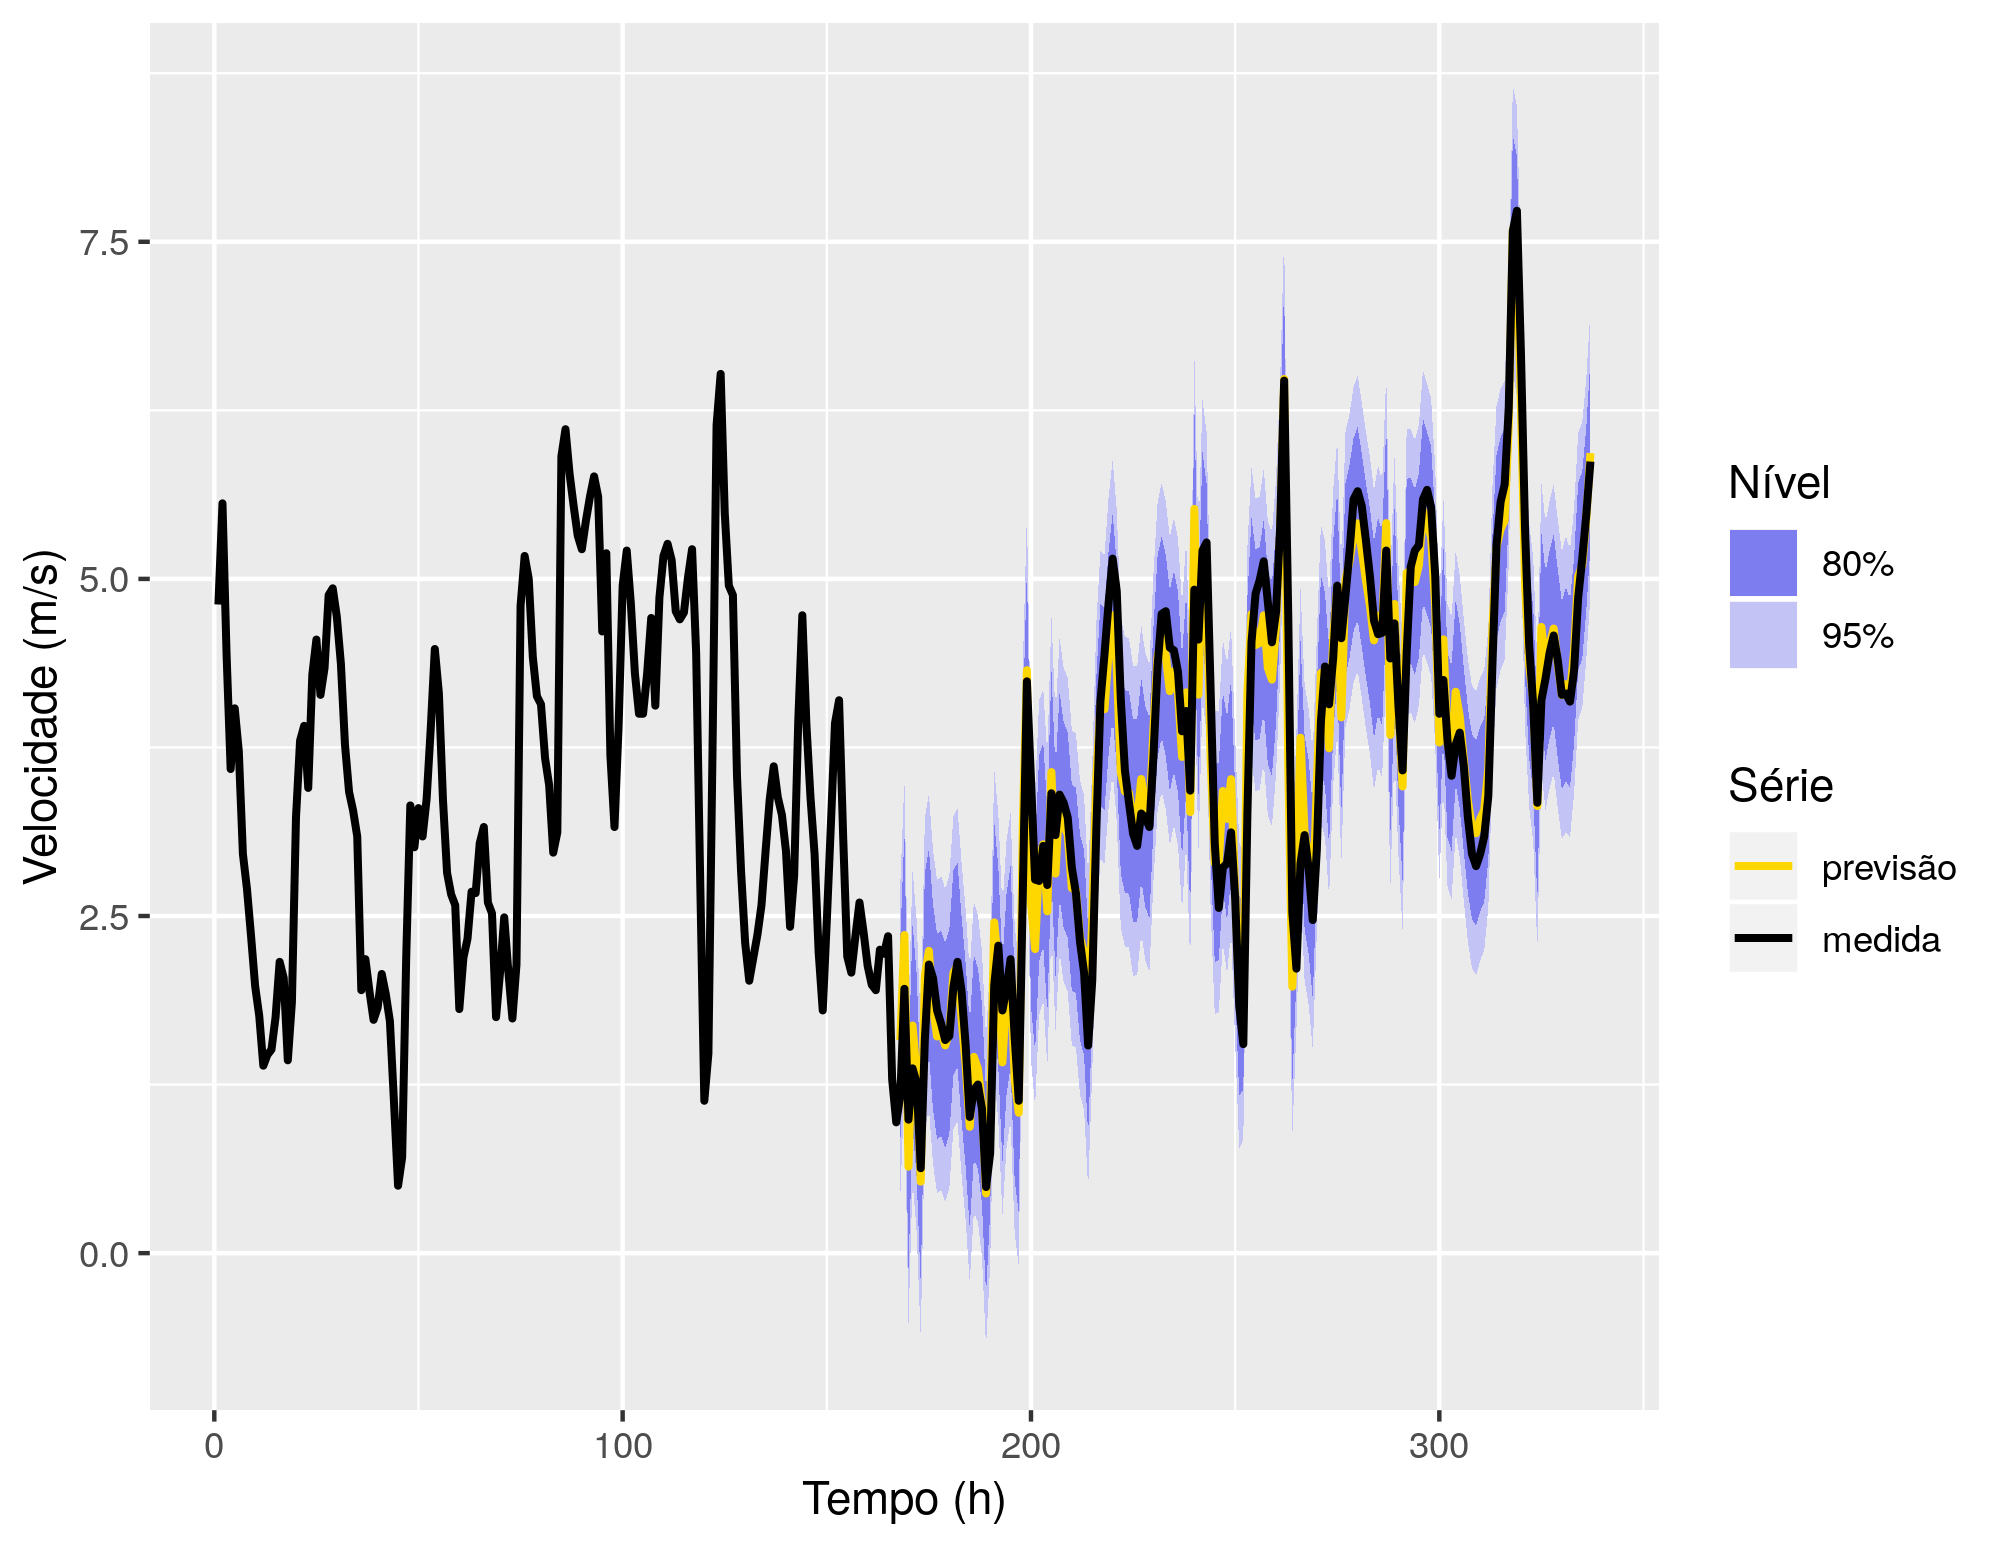
\includegraphics[width=\textwidth]{var_result}
		\caption{Evolução dos parâmetros p e q de um modelo ARIMA ao longo do tempo.}
	\end{figure}
\end{frame}

\begin{frame}
	\frametitle{Evolução dos parâmetros p e q de um modelo ARIMA ao longo do tempo.}
	\begin{figure}
		\centering
		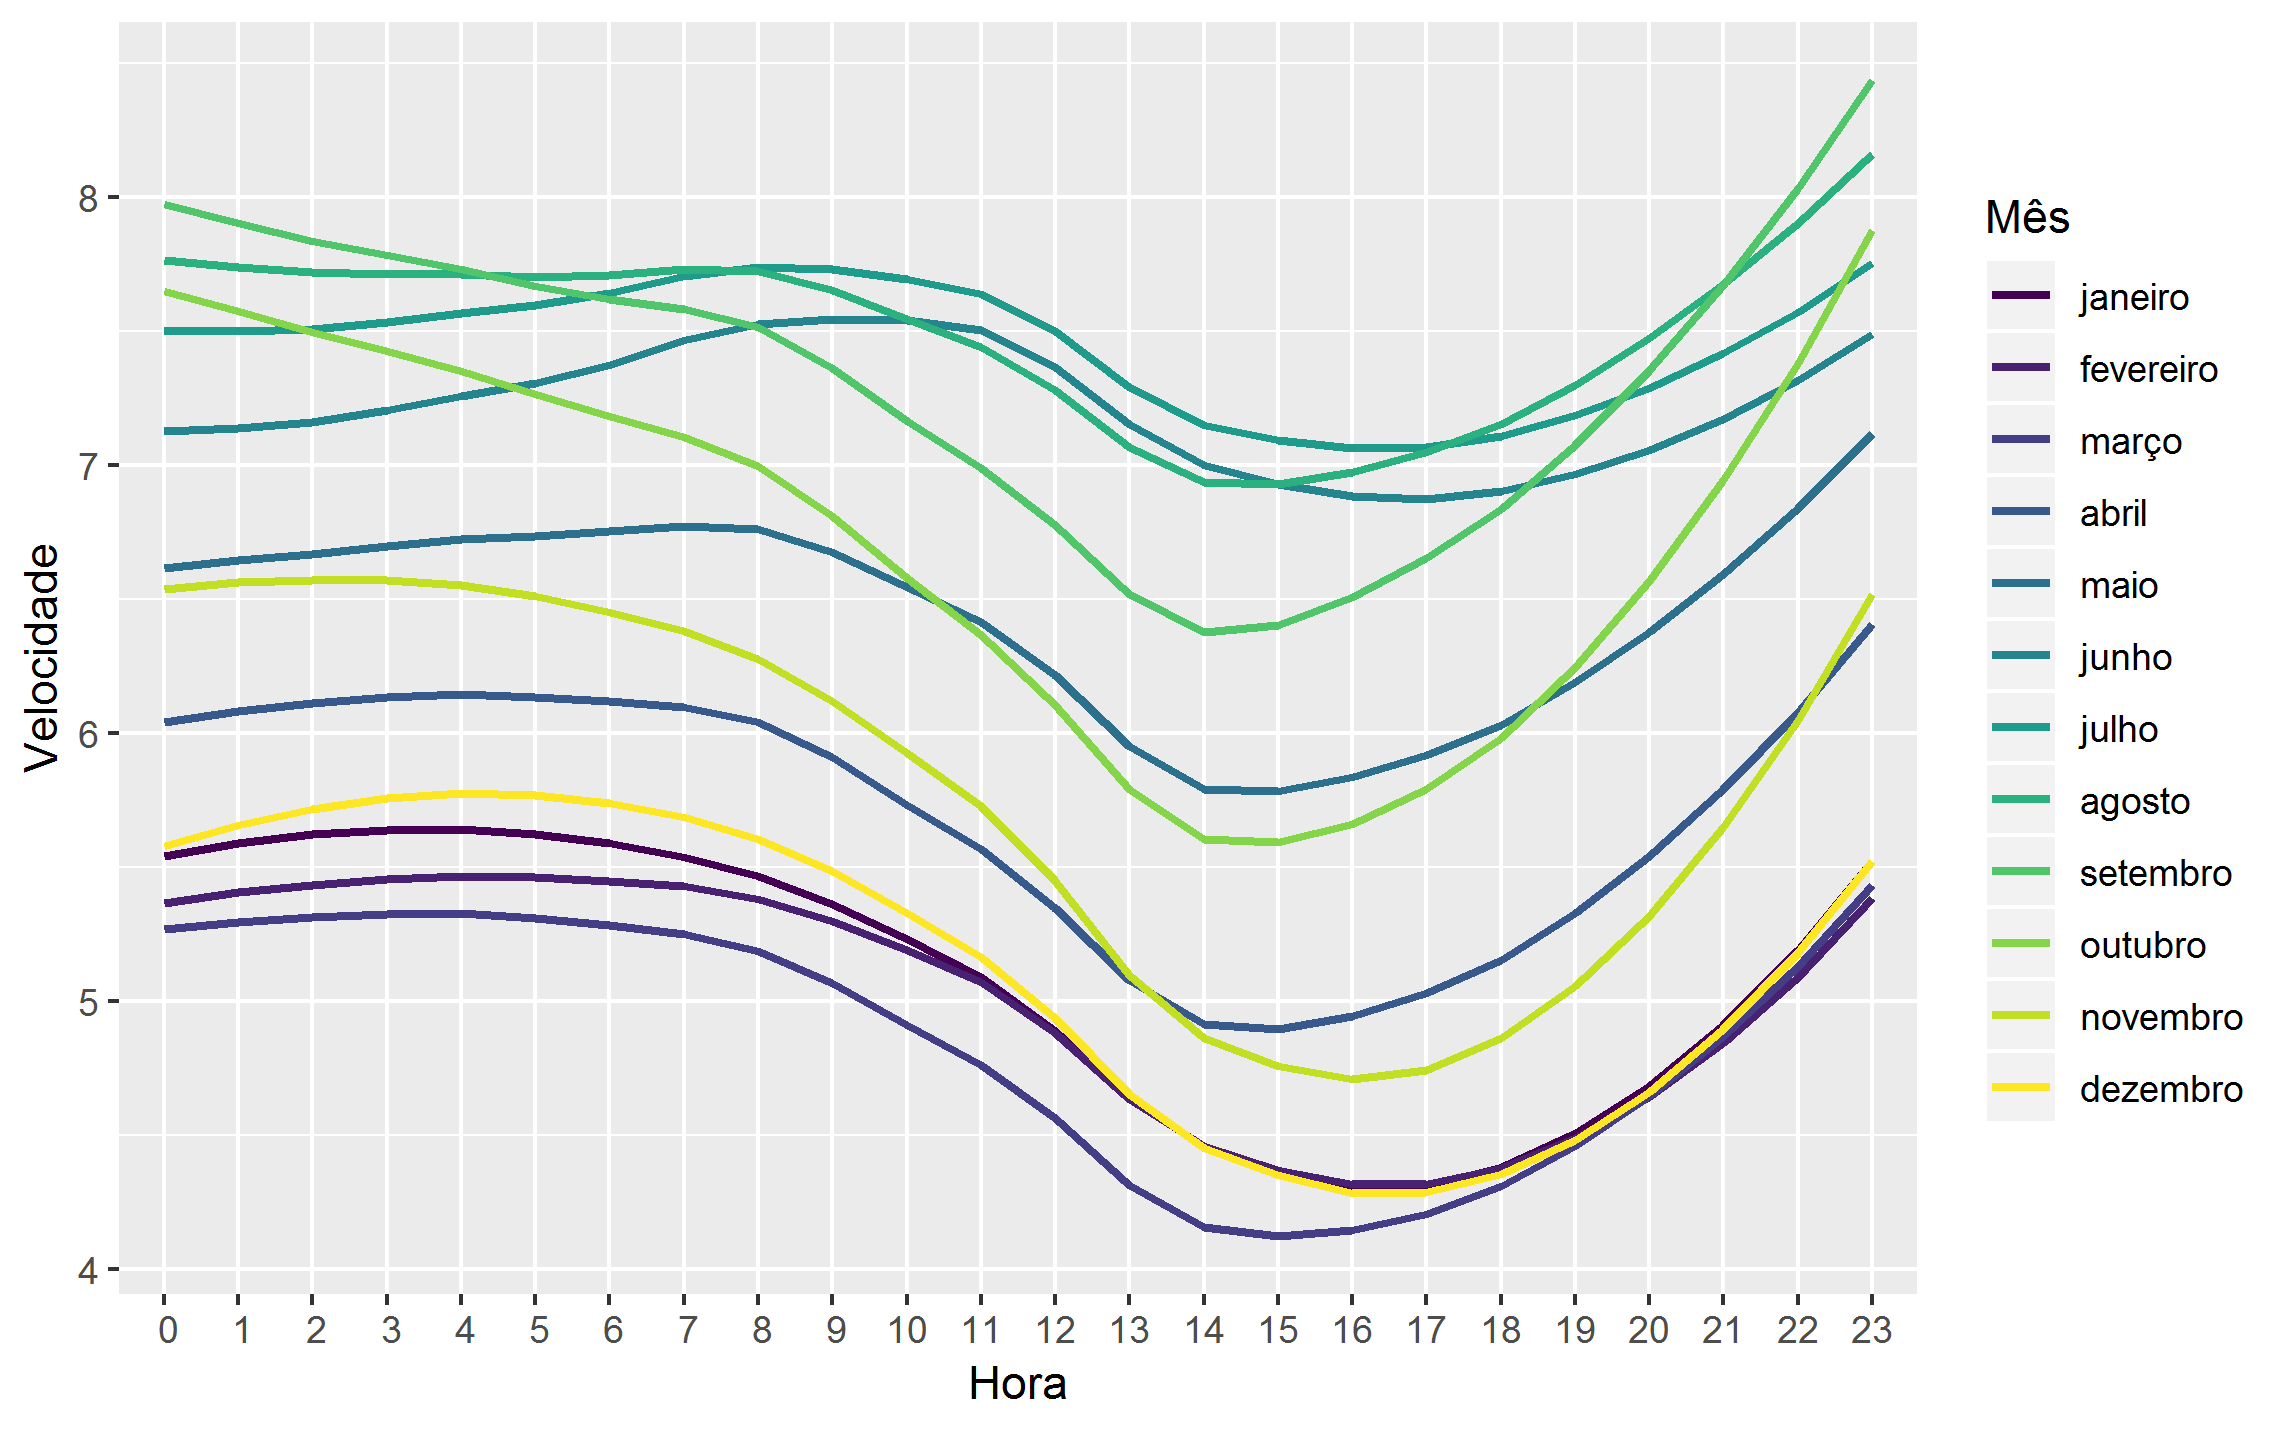
\includegraphics[width=\textwidth]{diurnal}
		\caption{Evolução dos parâmetros p e q de um modelo ARIMA ao longo do tempo.}
	\end{figure}
\end{frame}

\begin{frame}
	\frametitle{GARCH}
	\begin{figure}
		\centering
		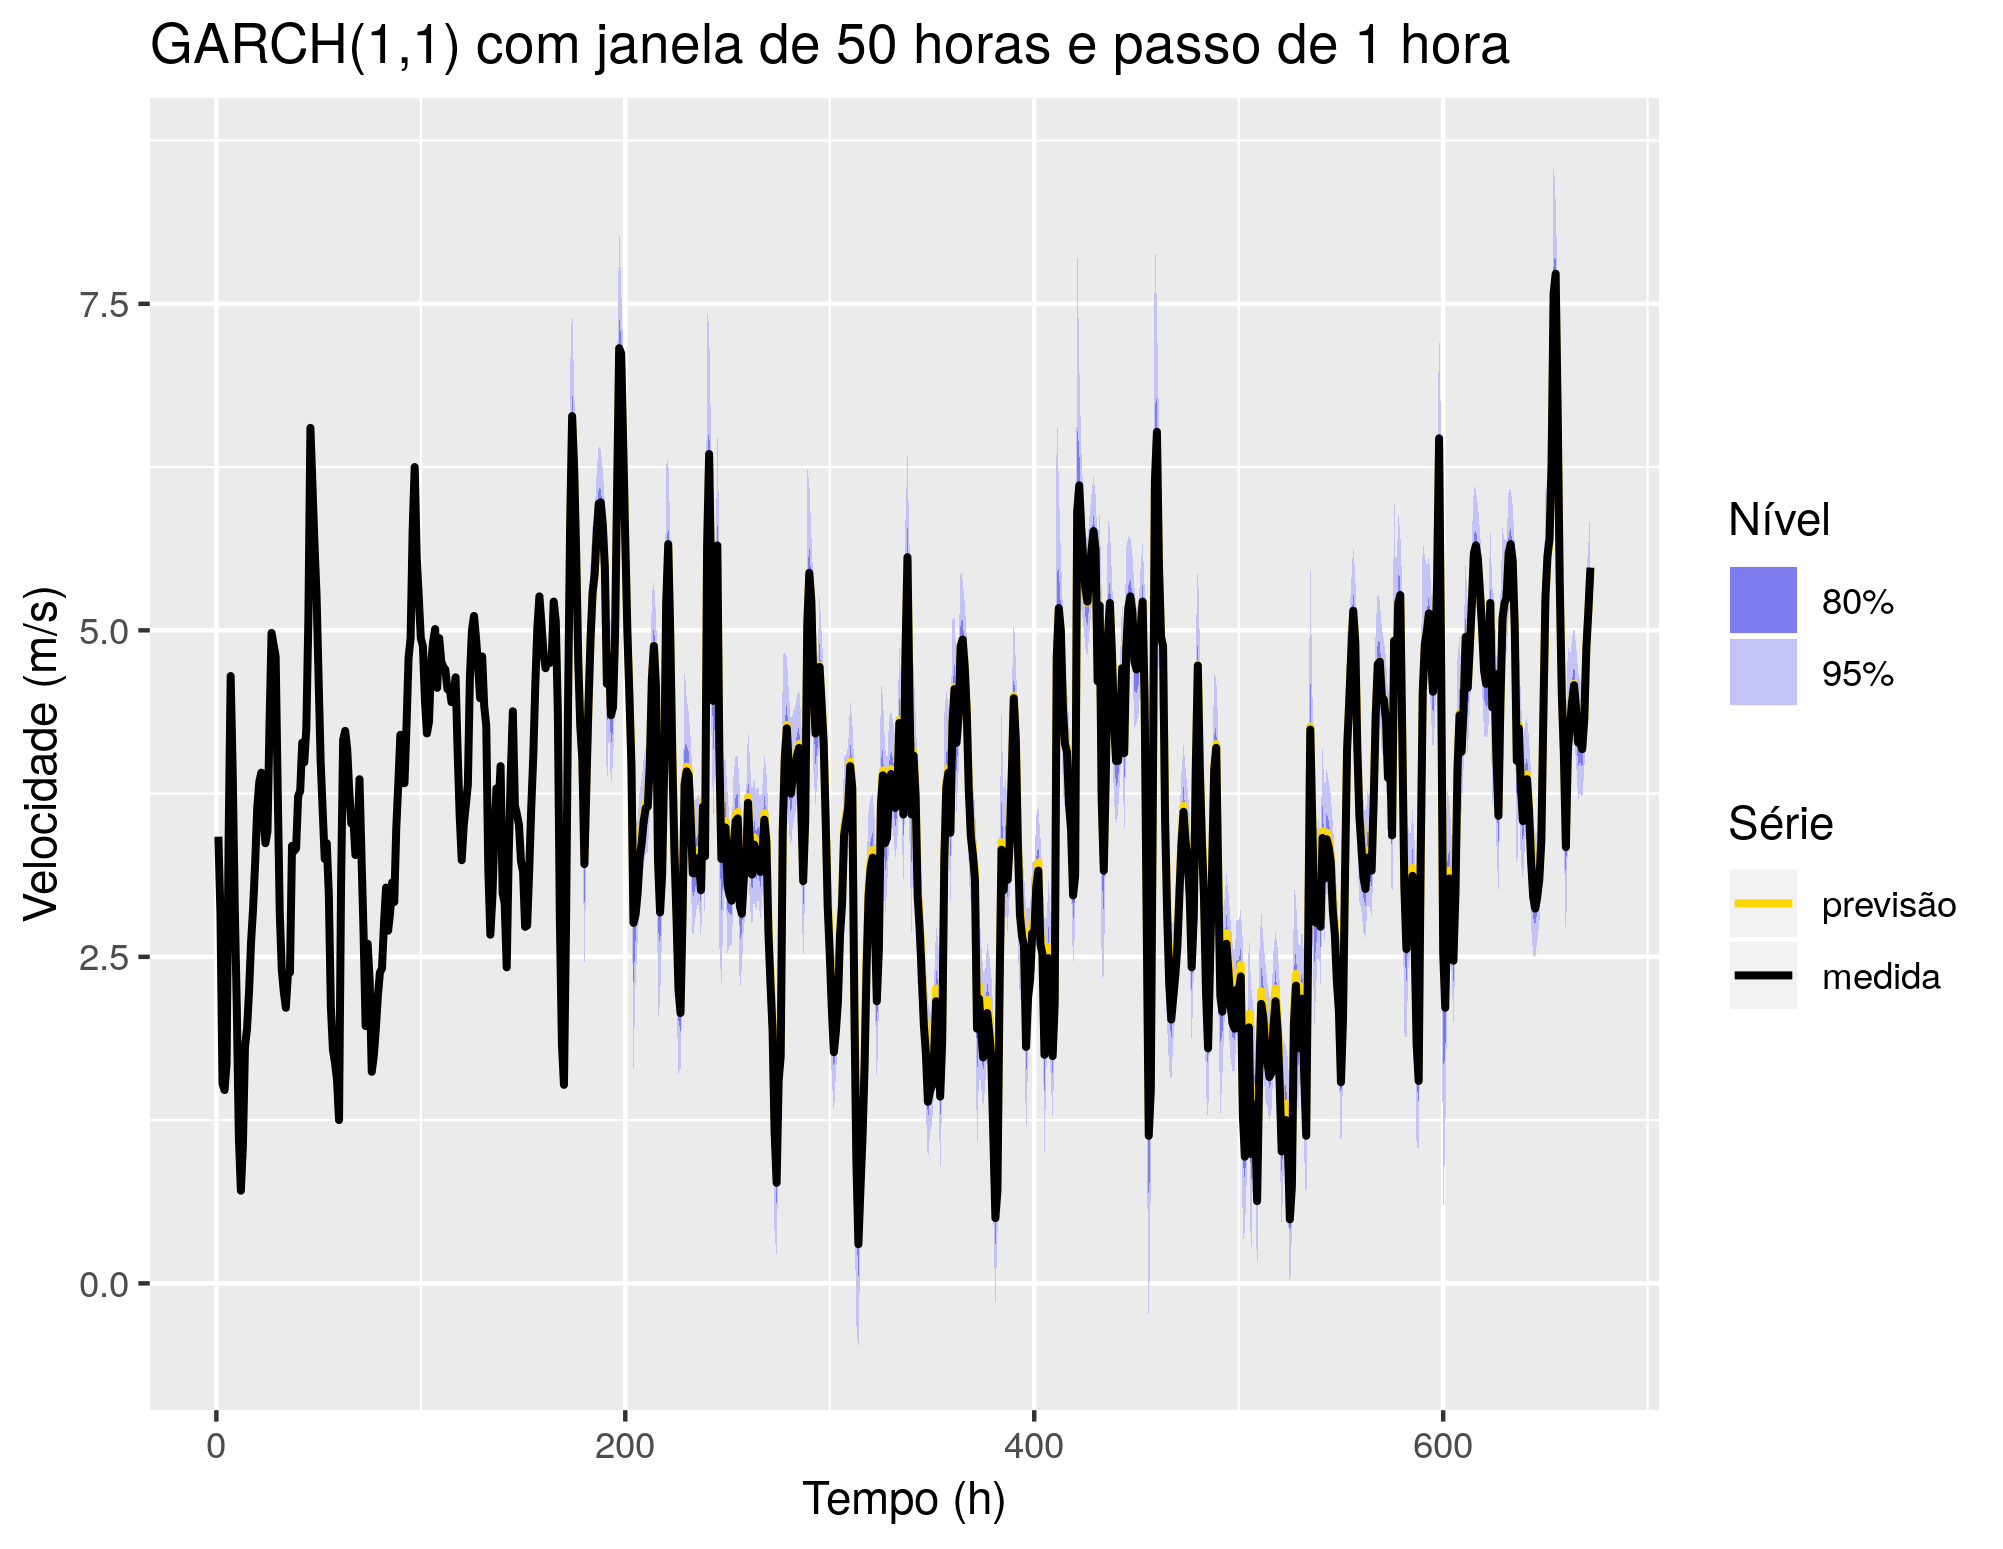
\includegraphics[width=\textwidth]{garch_first}
		\caption{GARCH}
	\end{figure}
\end{frame}

\begin{frame}
	\frametitle{GARCH}
	\begin{figure}
		\centering
		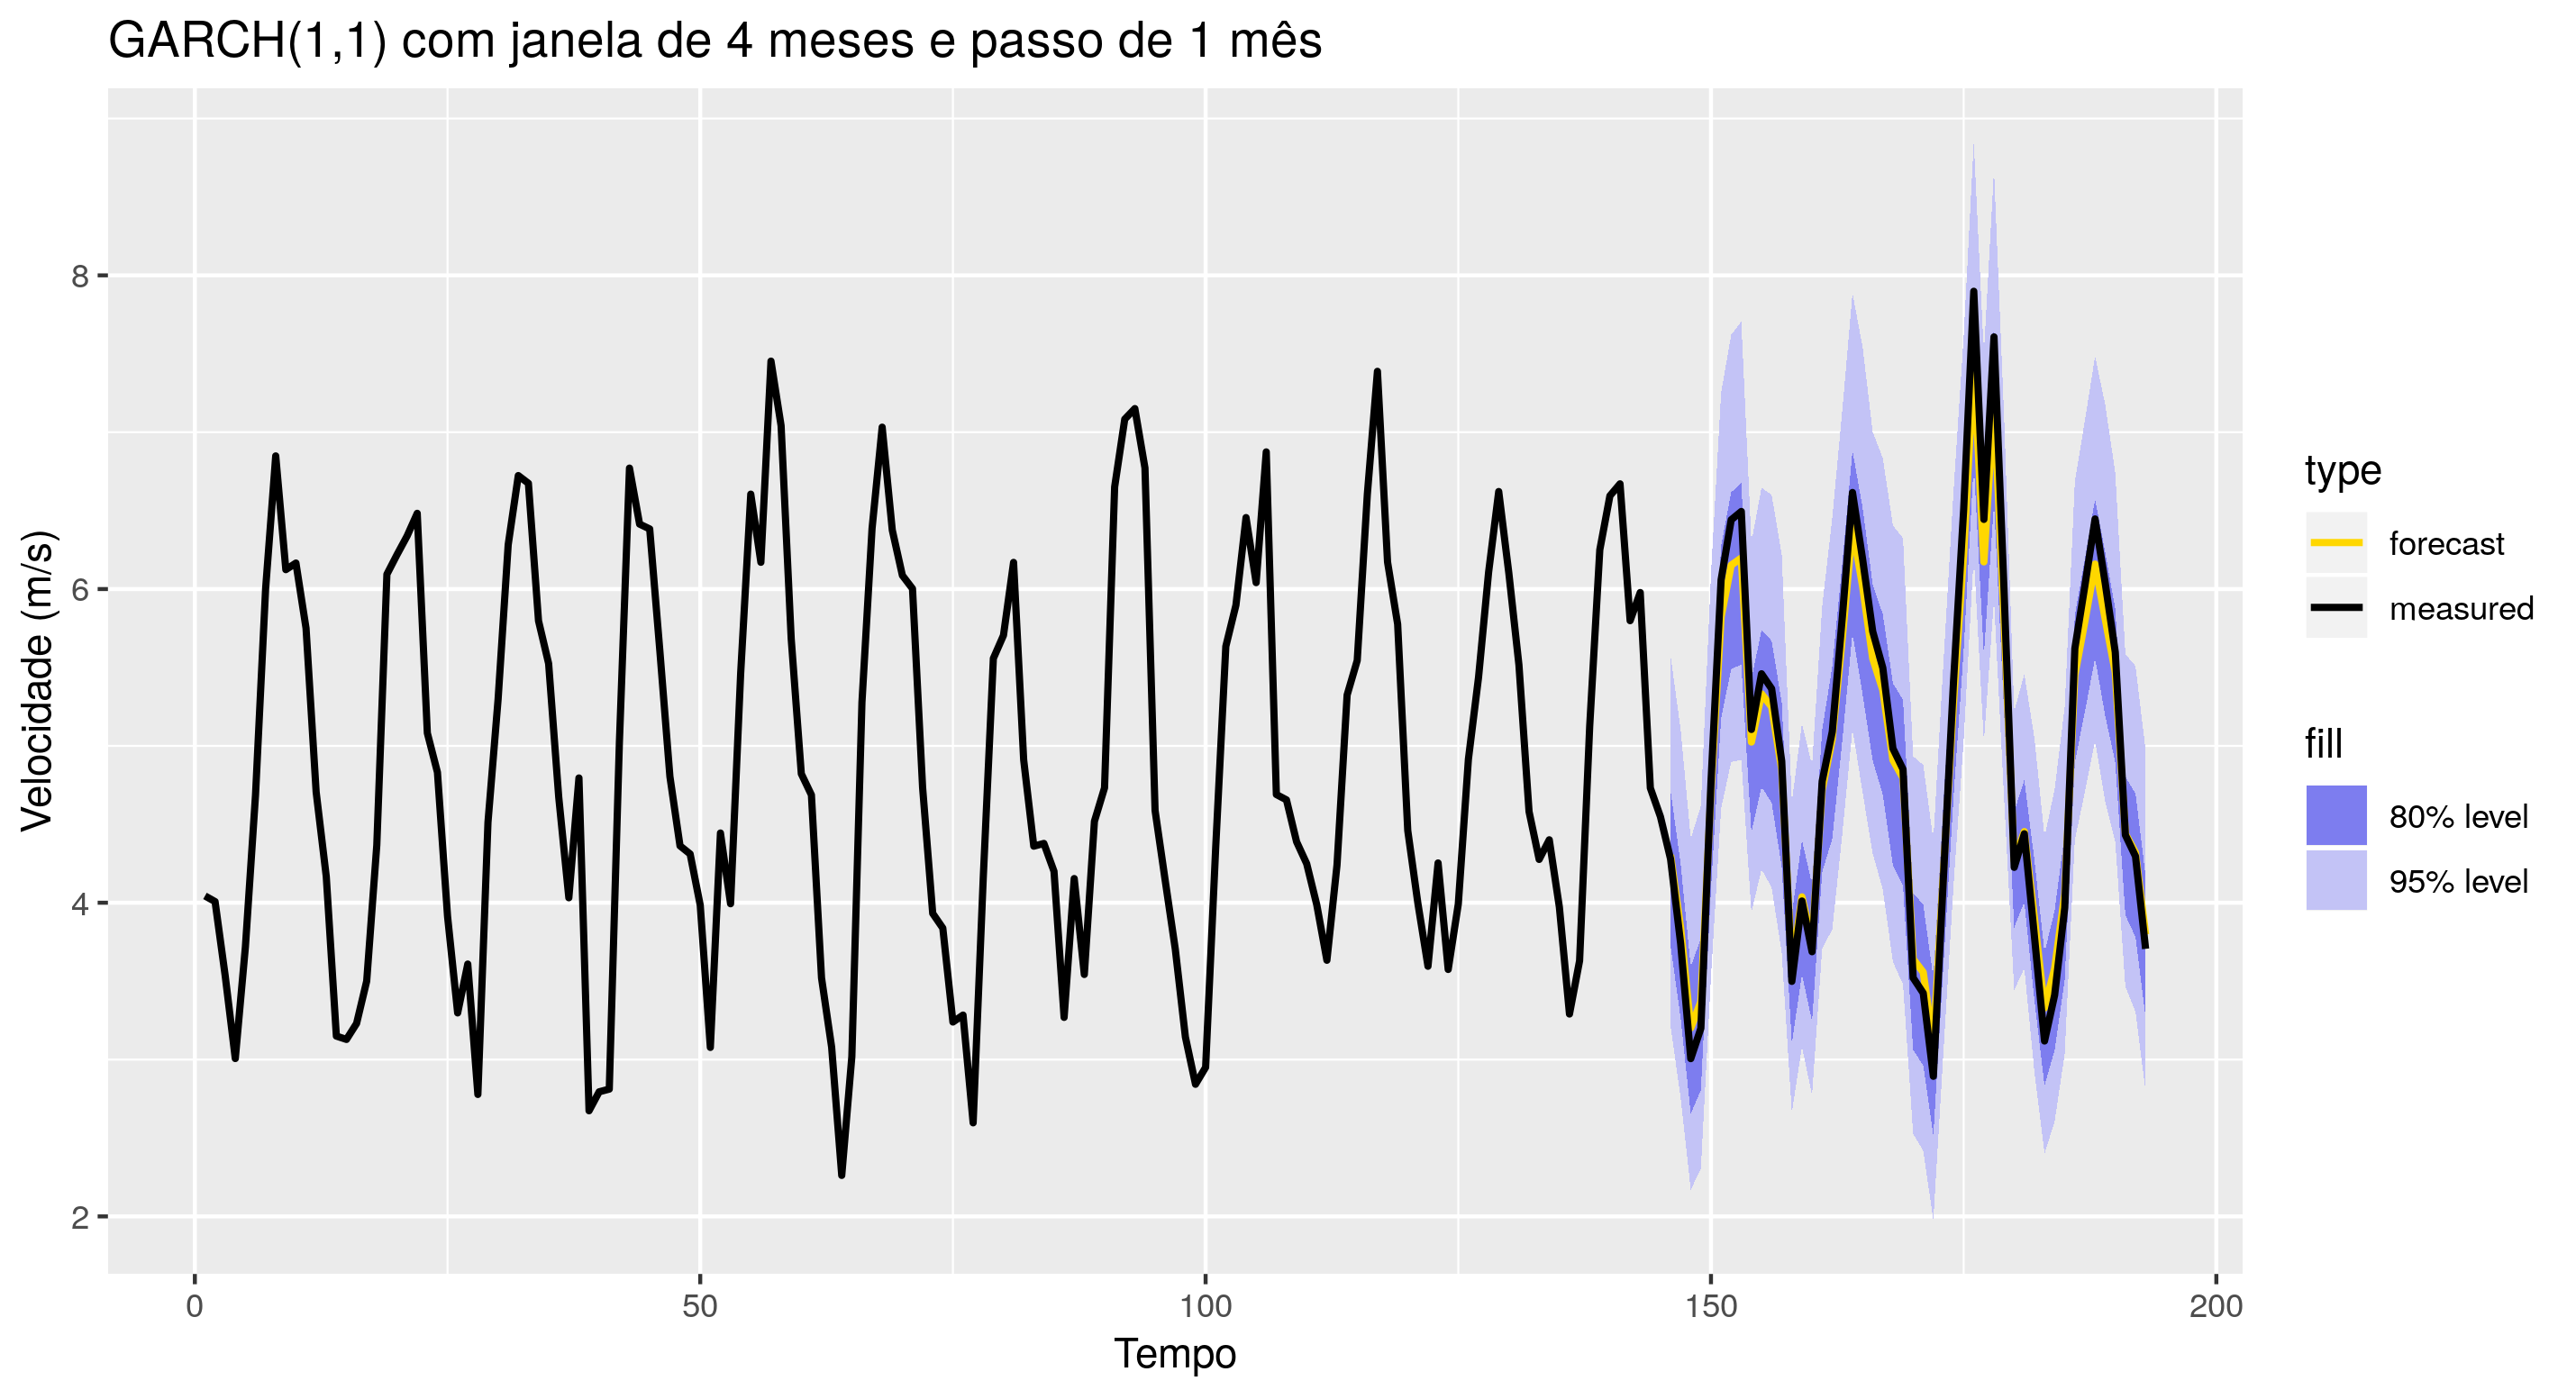
\includegraphics[width=\textwidth]{garch_month}
		\caption{GARCH}
	\end{figure}
\end{frame}

\begin{frame}
	\frametitle{Curva de potência de um aerogerador genérico.}
	\begin{figure}
		\centering
		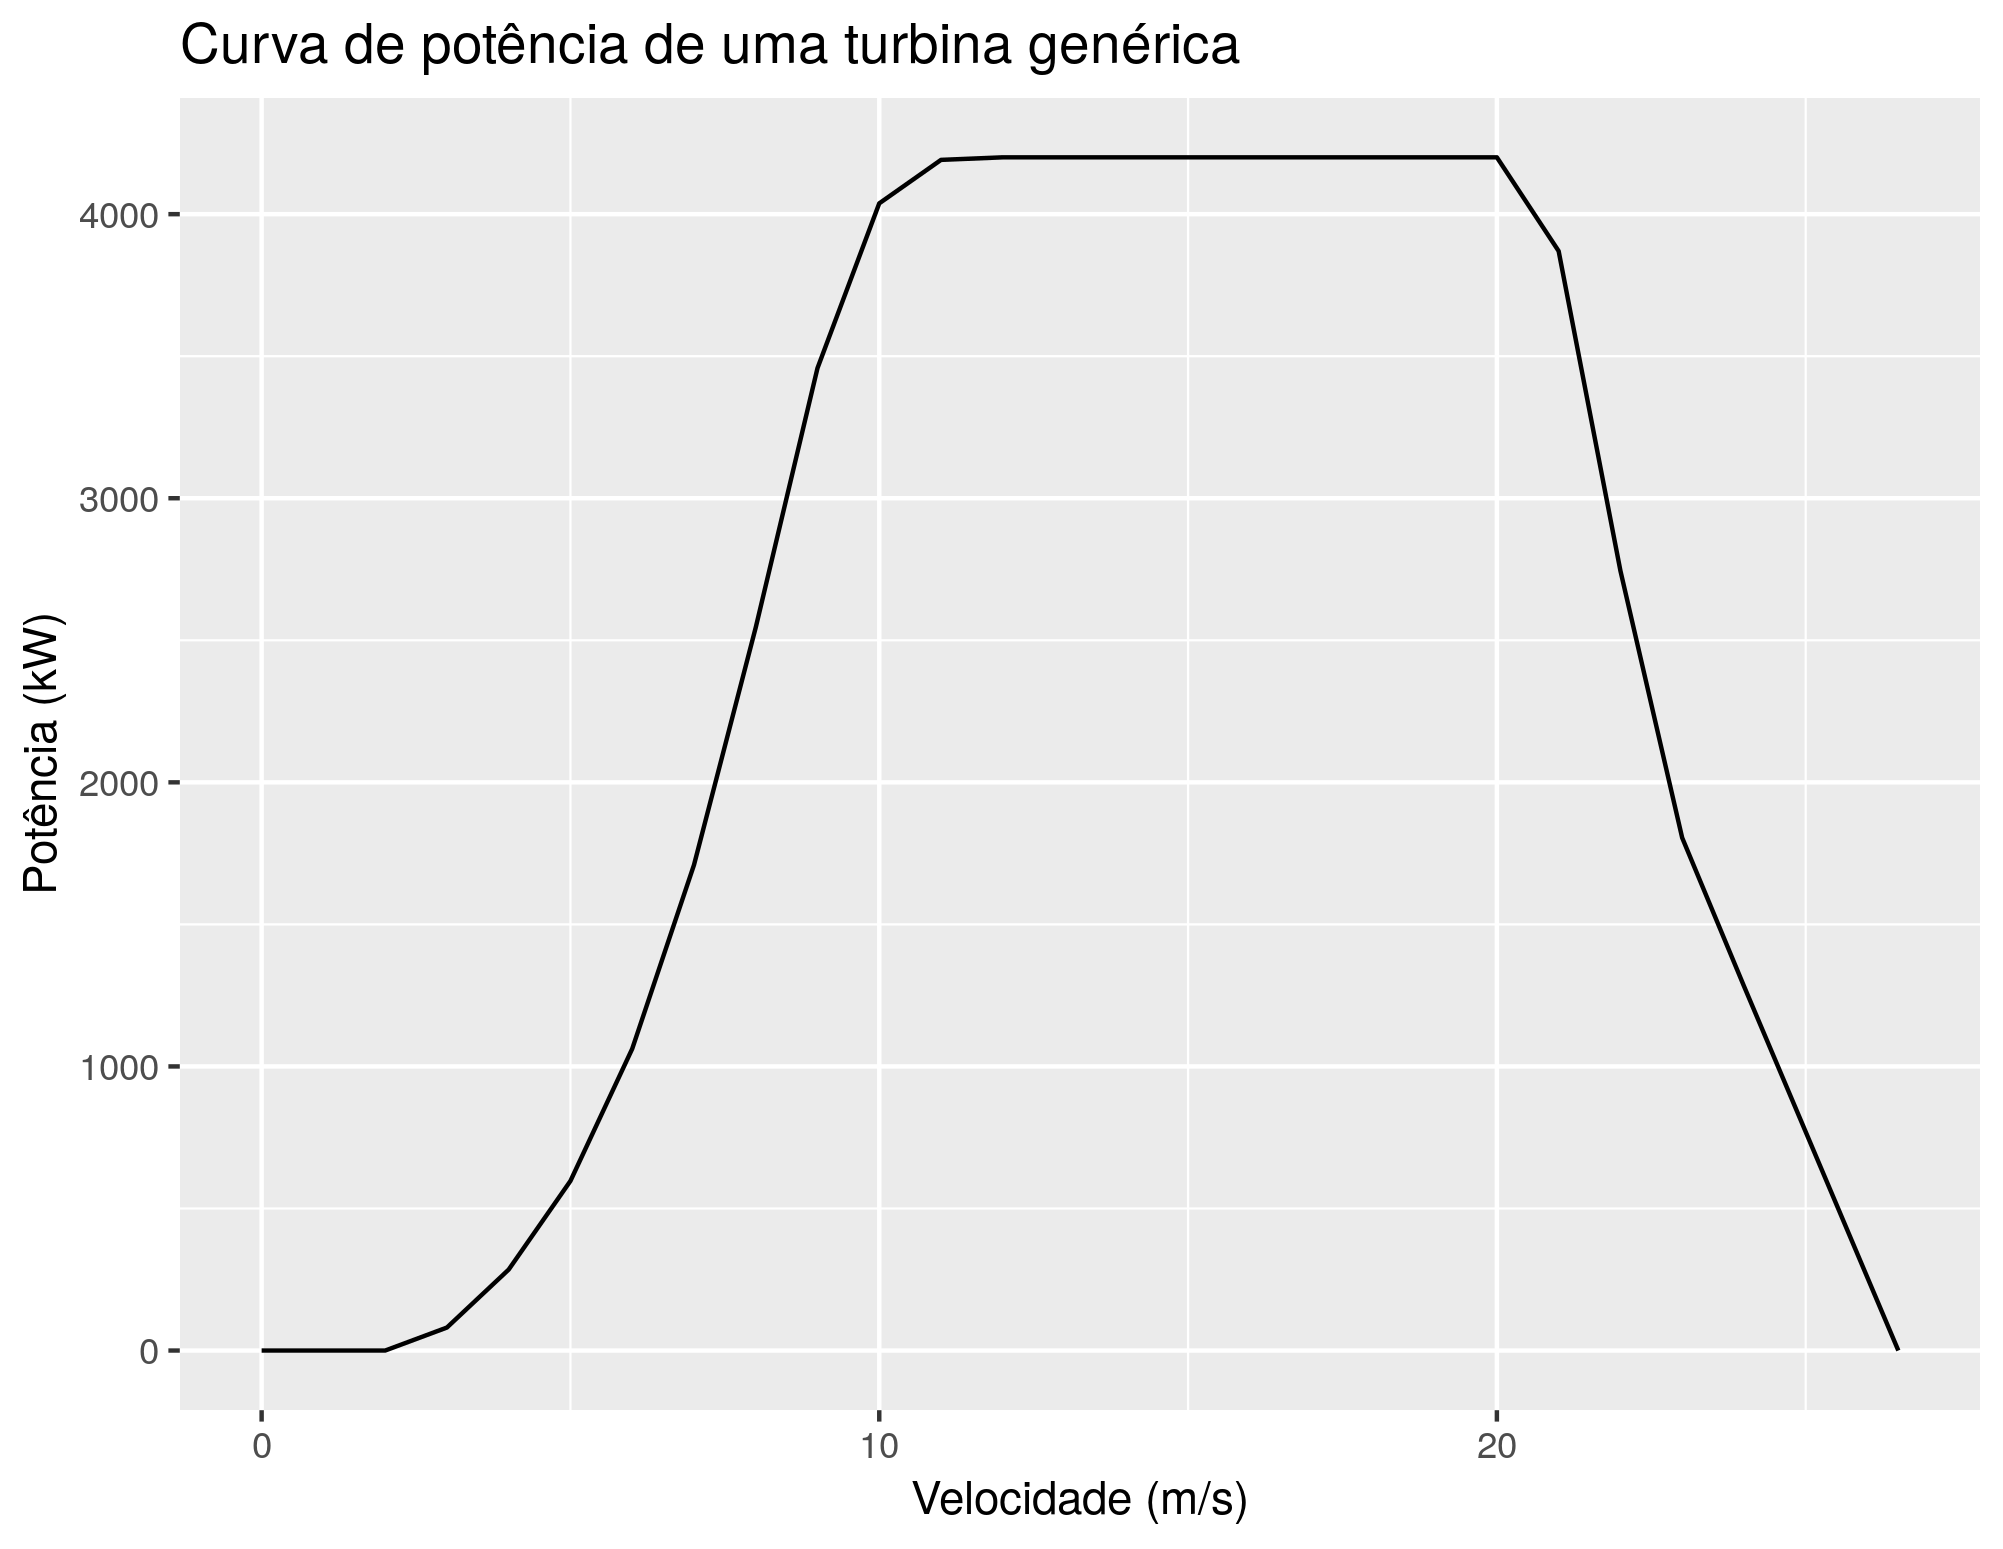
\includegraphics[width=\textwidth]{power_curve}
		\caption{Curva de potência de um aerogerador genérico.}
	\end{figure}
\end{frame}

\begin{frame}
	\frametitle{Curva de potência de um aerogerador genérico.}
	\begin{figure}
		\centering
		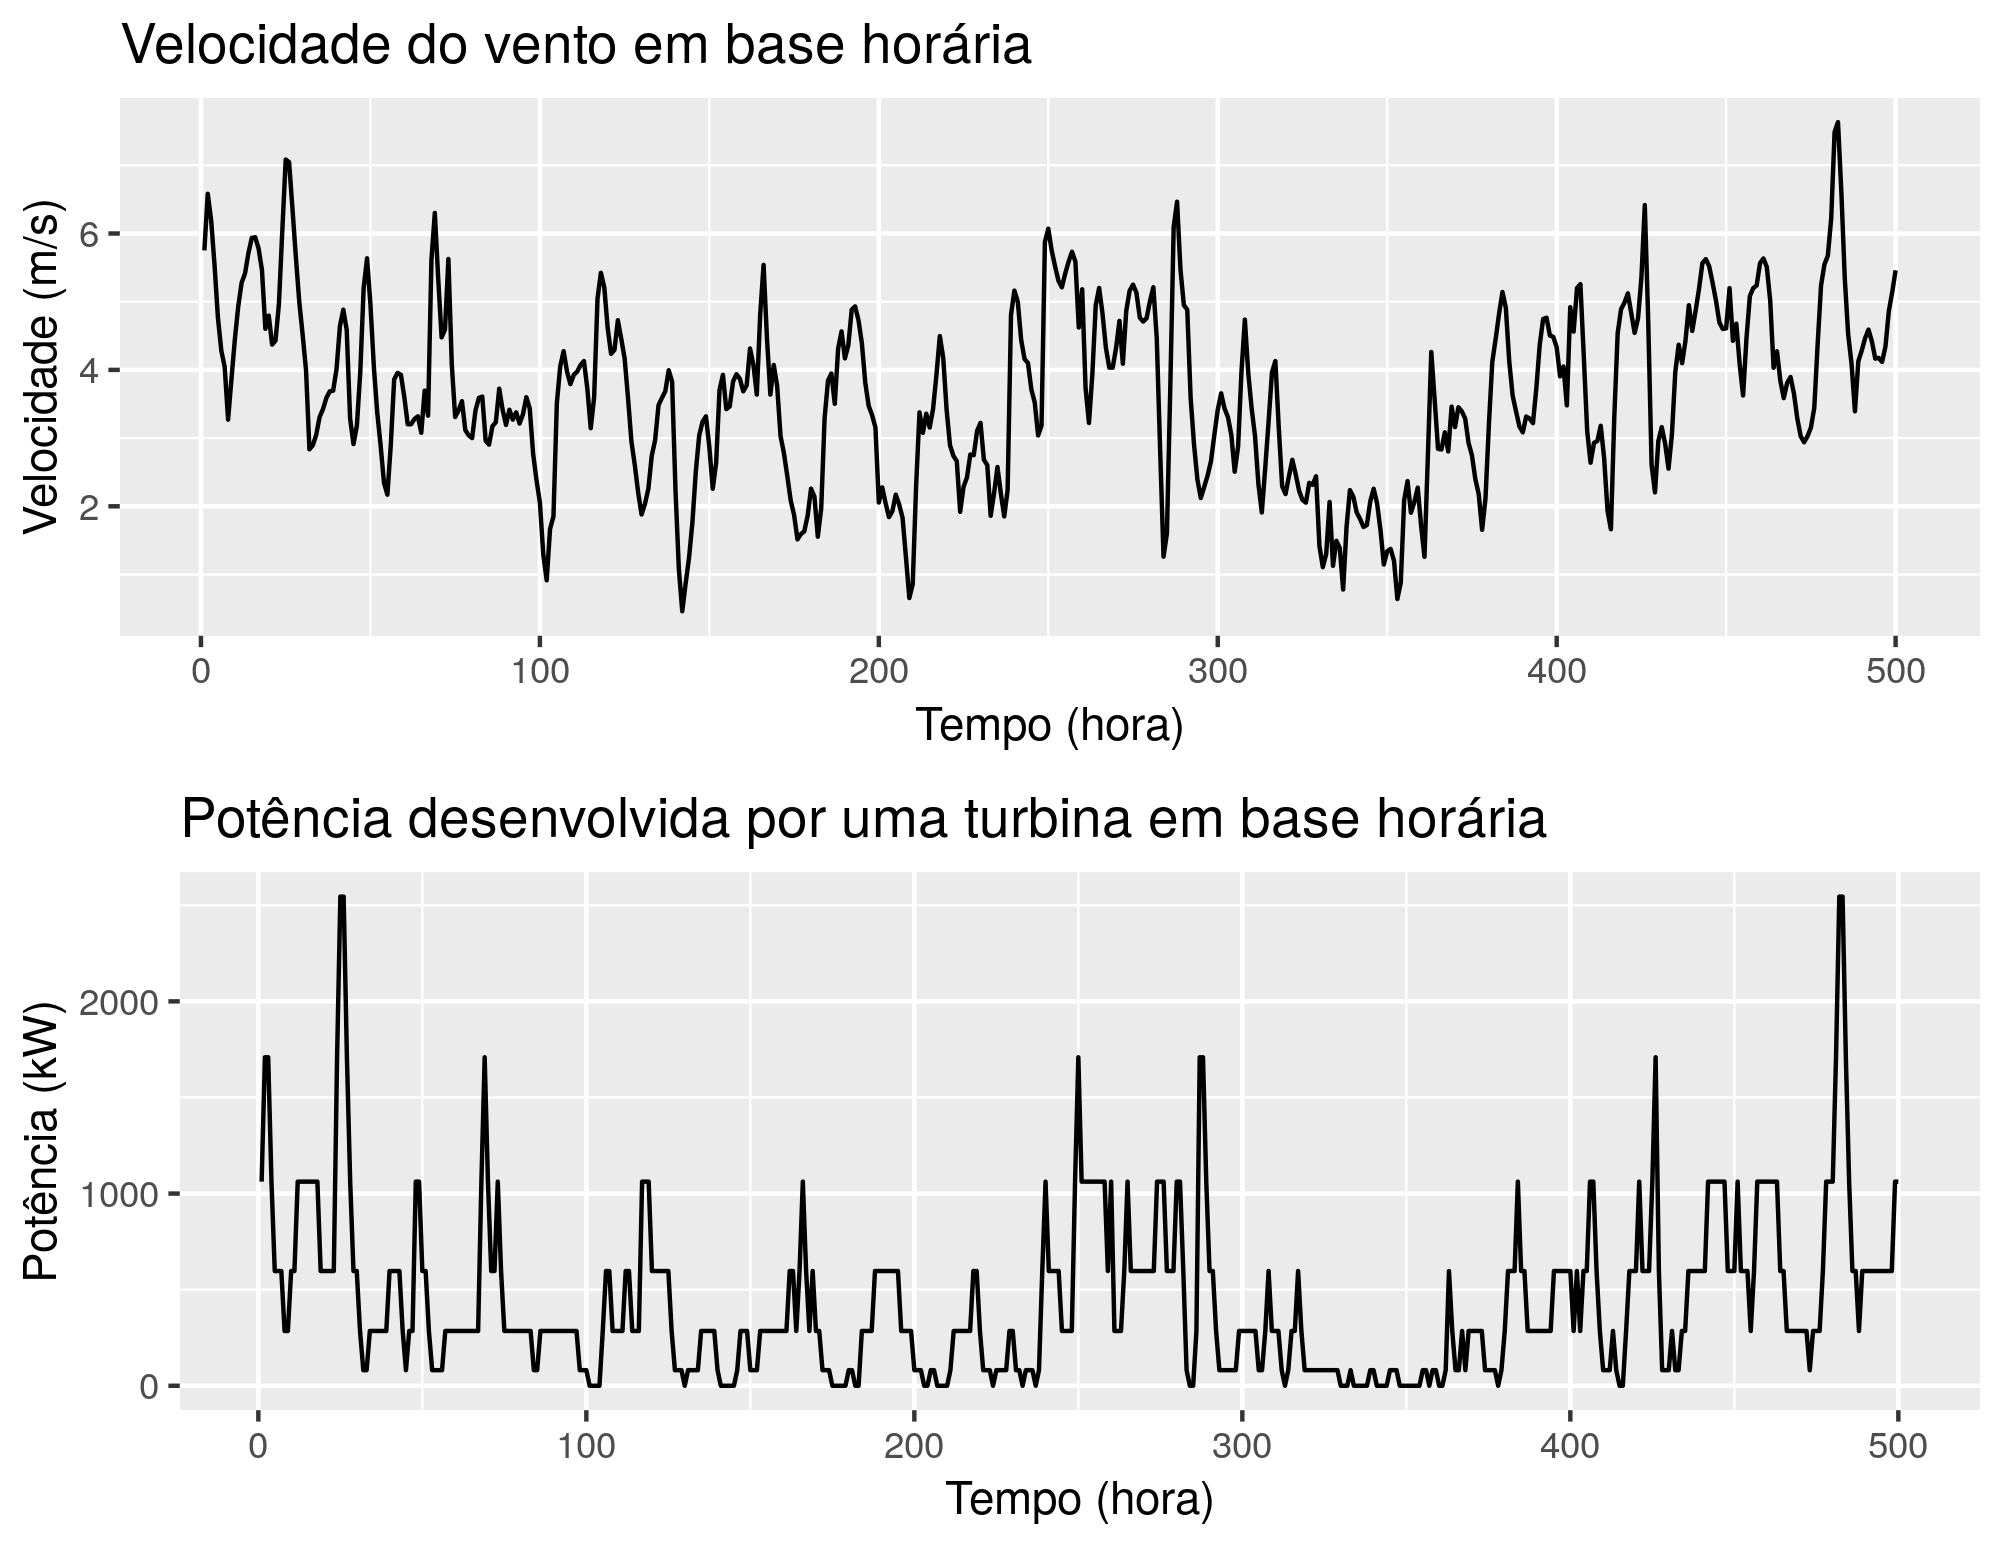
\includegraphics[width=\textwidth]{speed_power}
		\caption{Curva de potência de um aerogerador genérico.}
	\end{figure}
\end{frame}

\begin{frame}
	\frametitle{TDEF Map}
	\begin{figure}
		\centering
		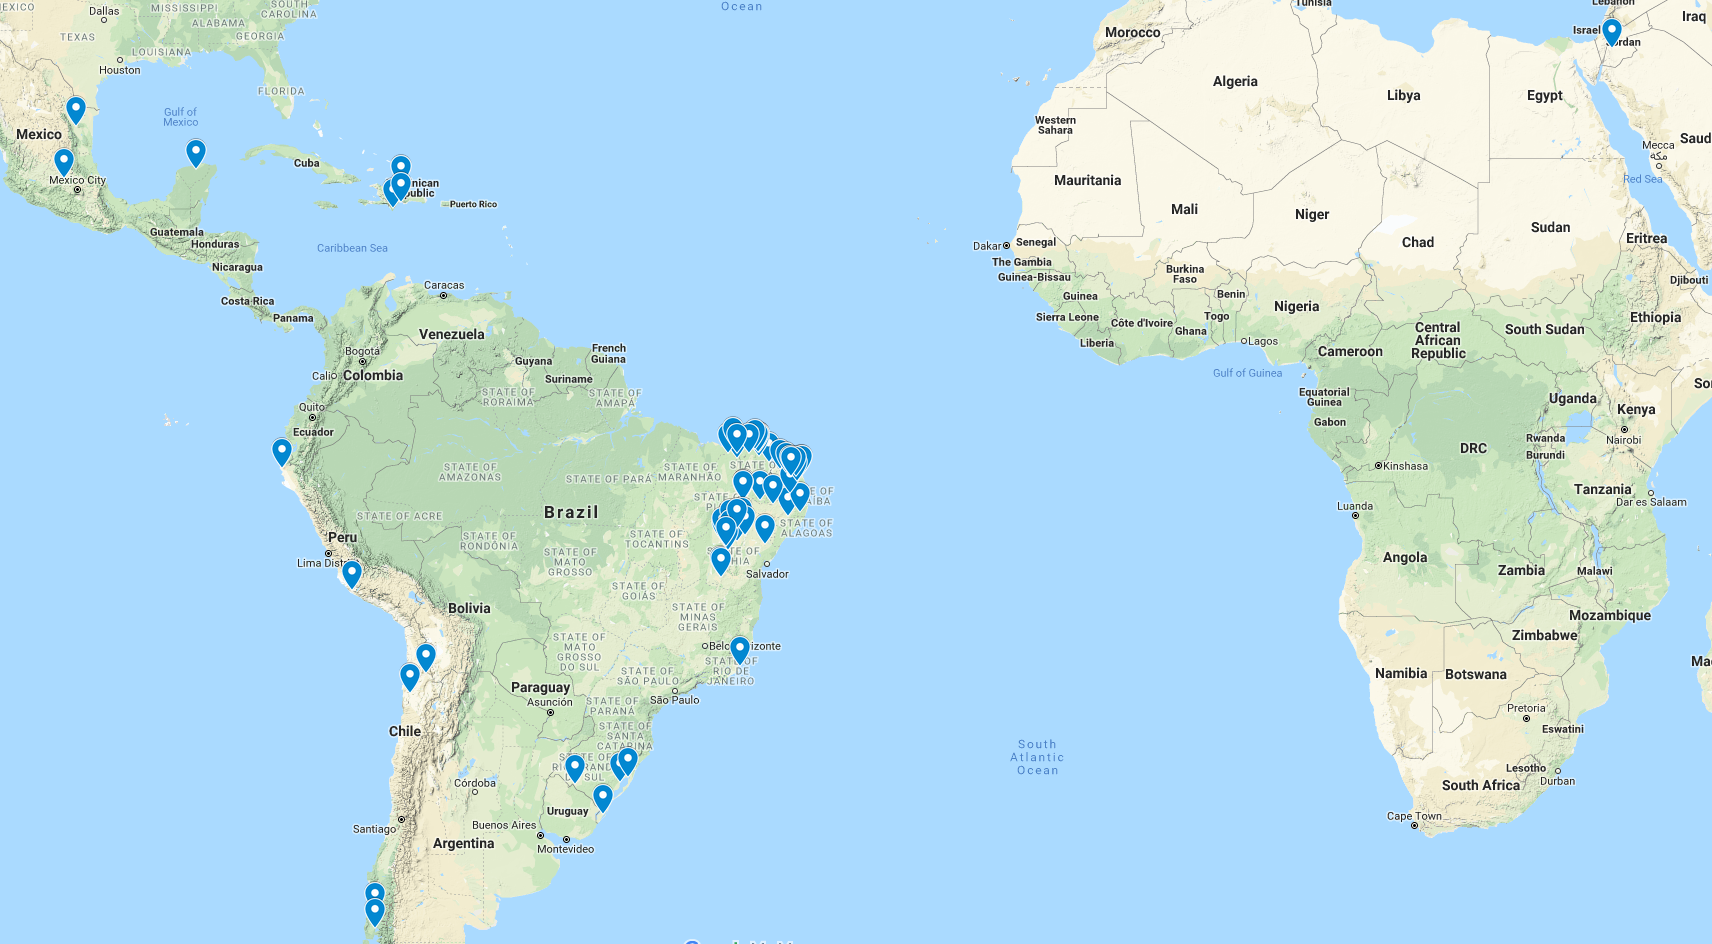
\includegraphics[width=\textwidth]{latam}
		\caption{TDEF Map}
	\end{figure}
\end{frame}


%#***********
%#* TDEF I: *    
%#***********

%    \AtBeginSection[]
%    {
%      \begin{frame}
%        \frametitle{Sumário}
%        \tableofcontents[currentsection]
%      \end{frame}
%    }
%    
%    \AtBeginSubsection[]
%    {
%      \begin{frame}
%        \frametitle{Sumário}
%        \tableofcontents[currentsection,currentsubsection]
%      \end{frame}
%    }

%{ 
%\usebackgroundtemplate{\includegraphics[width=\paperwidth,height=\paperheight]{osorio}} 


%\frame
%{
%	\frametitle{Energia eólica}        
%	O investimento em energia eólica vem crescendo em todo o mundo:\newline        
%	\begin{itemize}
%        \item Alternativa a fontes de energia não-renováveis
%        \item Capaz de suprir boa parte da demanda de um país
%        \item Economicamente viável
%        \item Décadas de experiência acumulada
%	\end{itemize}
%}

%\frame
%{
%	\frametitle{Energia eólica: em crescimento}
%	\begin{figure}[h]
%   \centering
%	\includegraphics[scale=0.47]{19802010}
%	\caption{Geração de energia. Fonte: EPE.}
%	\end{figure}
%}

%\frame
%{
%	\frametitle{O recurso eólico nacional}
%	\begin{figure}[h]
%   	\centering
%		\includegraphics[scale=0.5]{brasilpotencialeolico}
%		\caption{O potencial eólico do Brasil. Fonte: CEPEL.}
%	\end{figure}
%}

%\frame
%{
%	\frametitle{O cálculo da potência}
%	\begin{equation*}
%		P = \frac{1}{2}\rho \frac{\pi D^2}{4}\nu^3C_p\eta
%	\end{equation*}
%	
%	\begin{flalign*}
%	P &= \mbox{potência elétrica na altura do cubo rotor}\left[W\right]&&\\
%	\rho &= \mbox{densidade do ar}\left[\frac{kg}{m^3}\right]&&\\
%	D &= \mbox{diâmetro do rotor}\left[m\right]&&\\\nonumber
%	\nu &= \mbox{velocidade do vento} \left[\frac{m}{s}\right]&&\\\nonumber
%	C_p &= \mbox{coeficiente aerodinâmico de potência do rotor}\left[W\right]&&\\\nonumber
%	\eta &= \mbox{eficiência do conjunto gerador/transmissão}&&\\\nonumber
%	\end{flalign*}
%}

%\frame
%{
%	\frametitle{Consumo médio residencial}
%	\begin{figure}[h]
%    	\centering
%		\includegraphics[width=\textwidth]{consumoresidencial}
%		\caption{Consumo médio residencial no país. Fonte: EPE.}
%	\end{figure}
%}

%\frame
%{
%	\frametitle{Dados de vento ERA 5: cidade de Sento Sé}
%	\begin{figure}[h]
%   	\centering
%		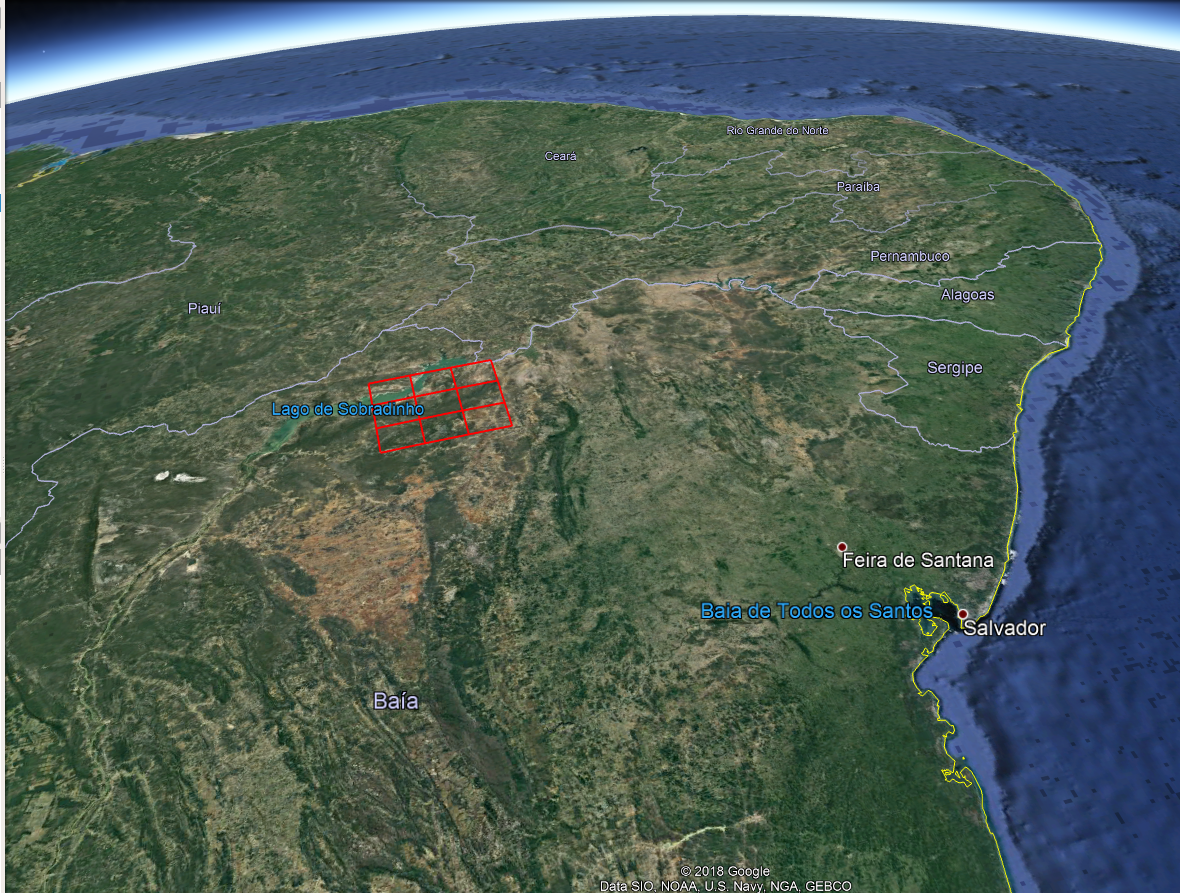
\includegraphics[scale=0.6]{earth}
%		\caption{Localização da região de medição por satélite da cidade de Sento Sé. Fonte: SIO, NOAA, U.S. Navy, NGA, GEBCO. \textcopyright \  2018 Google}
%	\end{figure}
%}

%\frame
%{
%	\frametitle{Rosa dos ventos anual}
%	\begin{figure}[h]
 %   	\centering
%		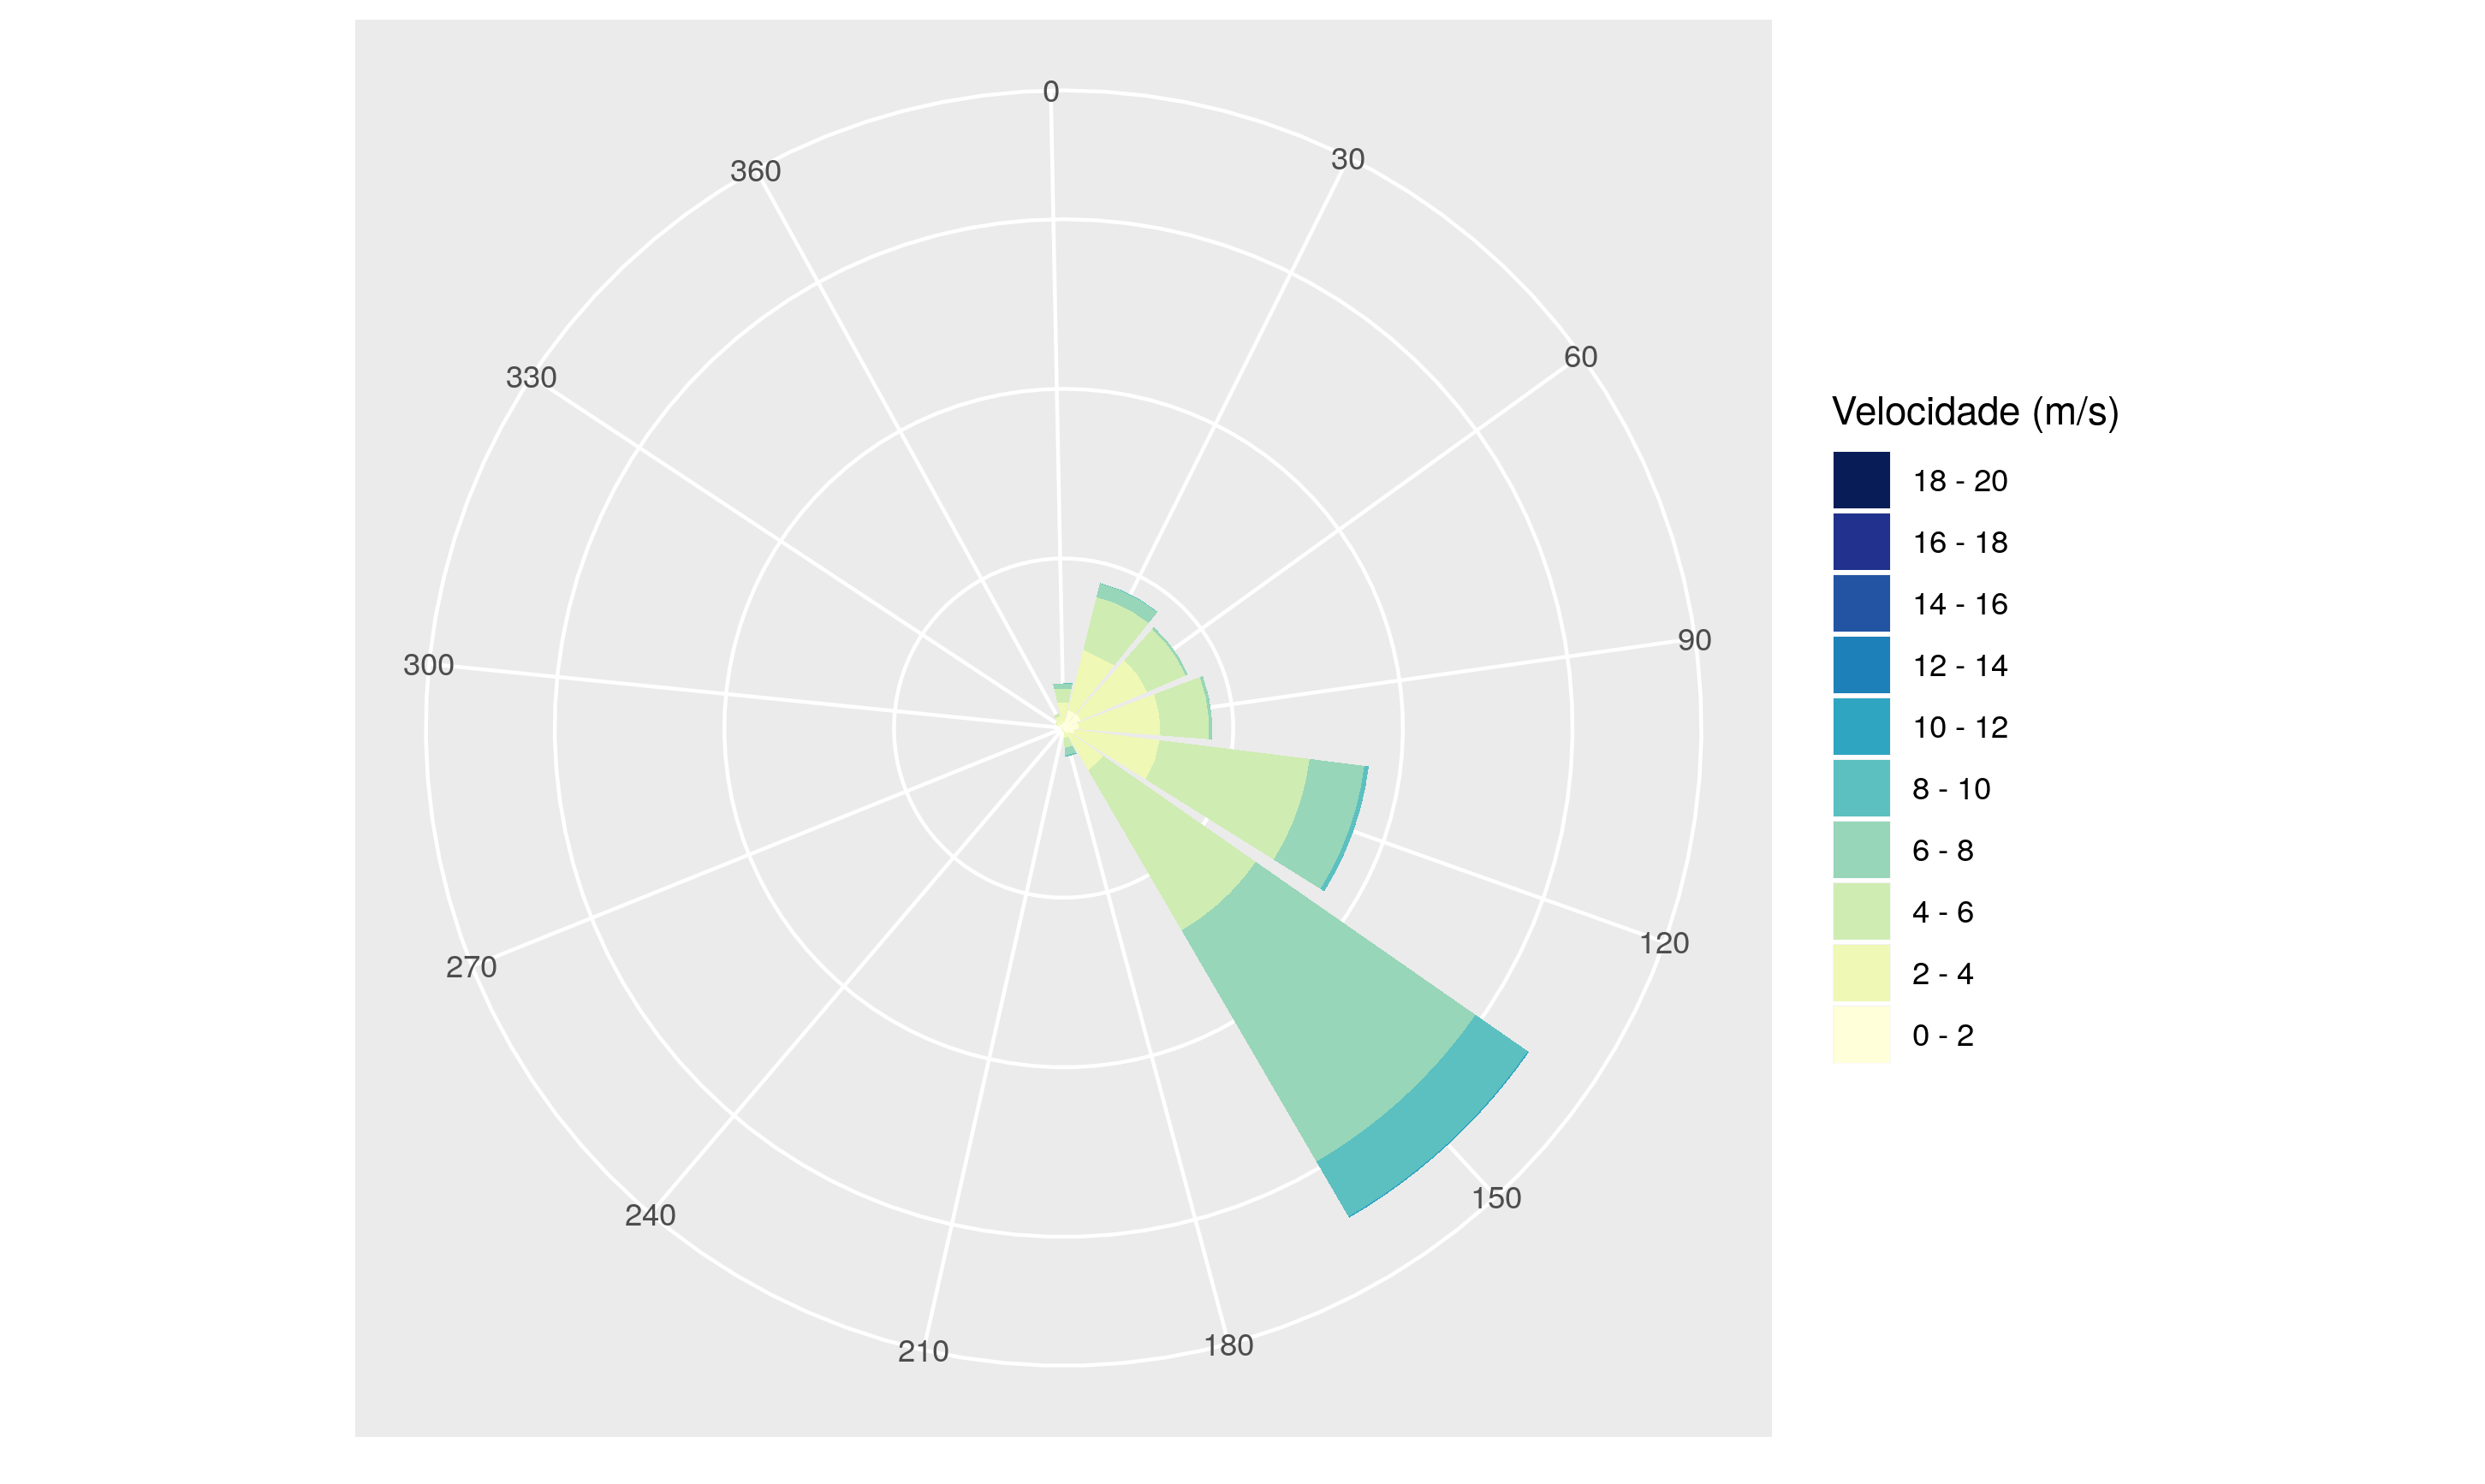
\includegraphics[scale=0.55]{windrose}
%		\caption{Rosa dos ventos do recurso eólico da cidade de Sento Sé no norte da Bahia. Fonte: autoria própria, dados: ECWMF.}
%	\end{figure}
%}

%\frame
%{
%	\frametitle{Rosas dos ventos mensais}
%	\begin{figure}[h]
%    	\centering
%  		\hspace*{-1.4cm}   
%   	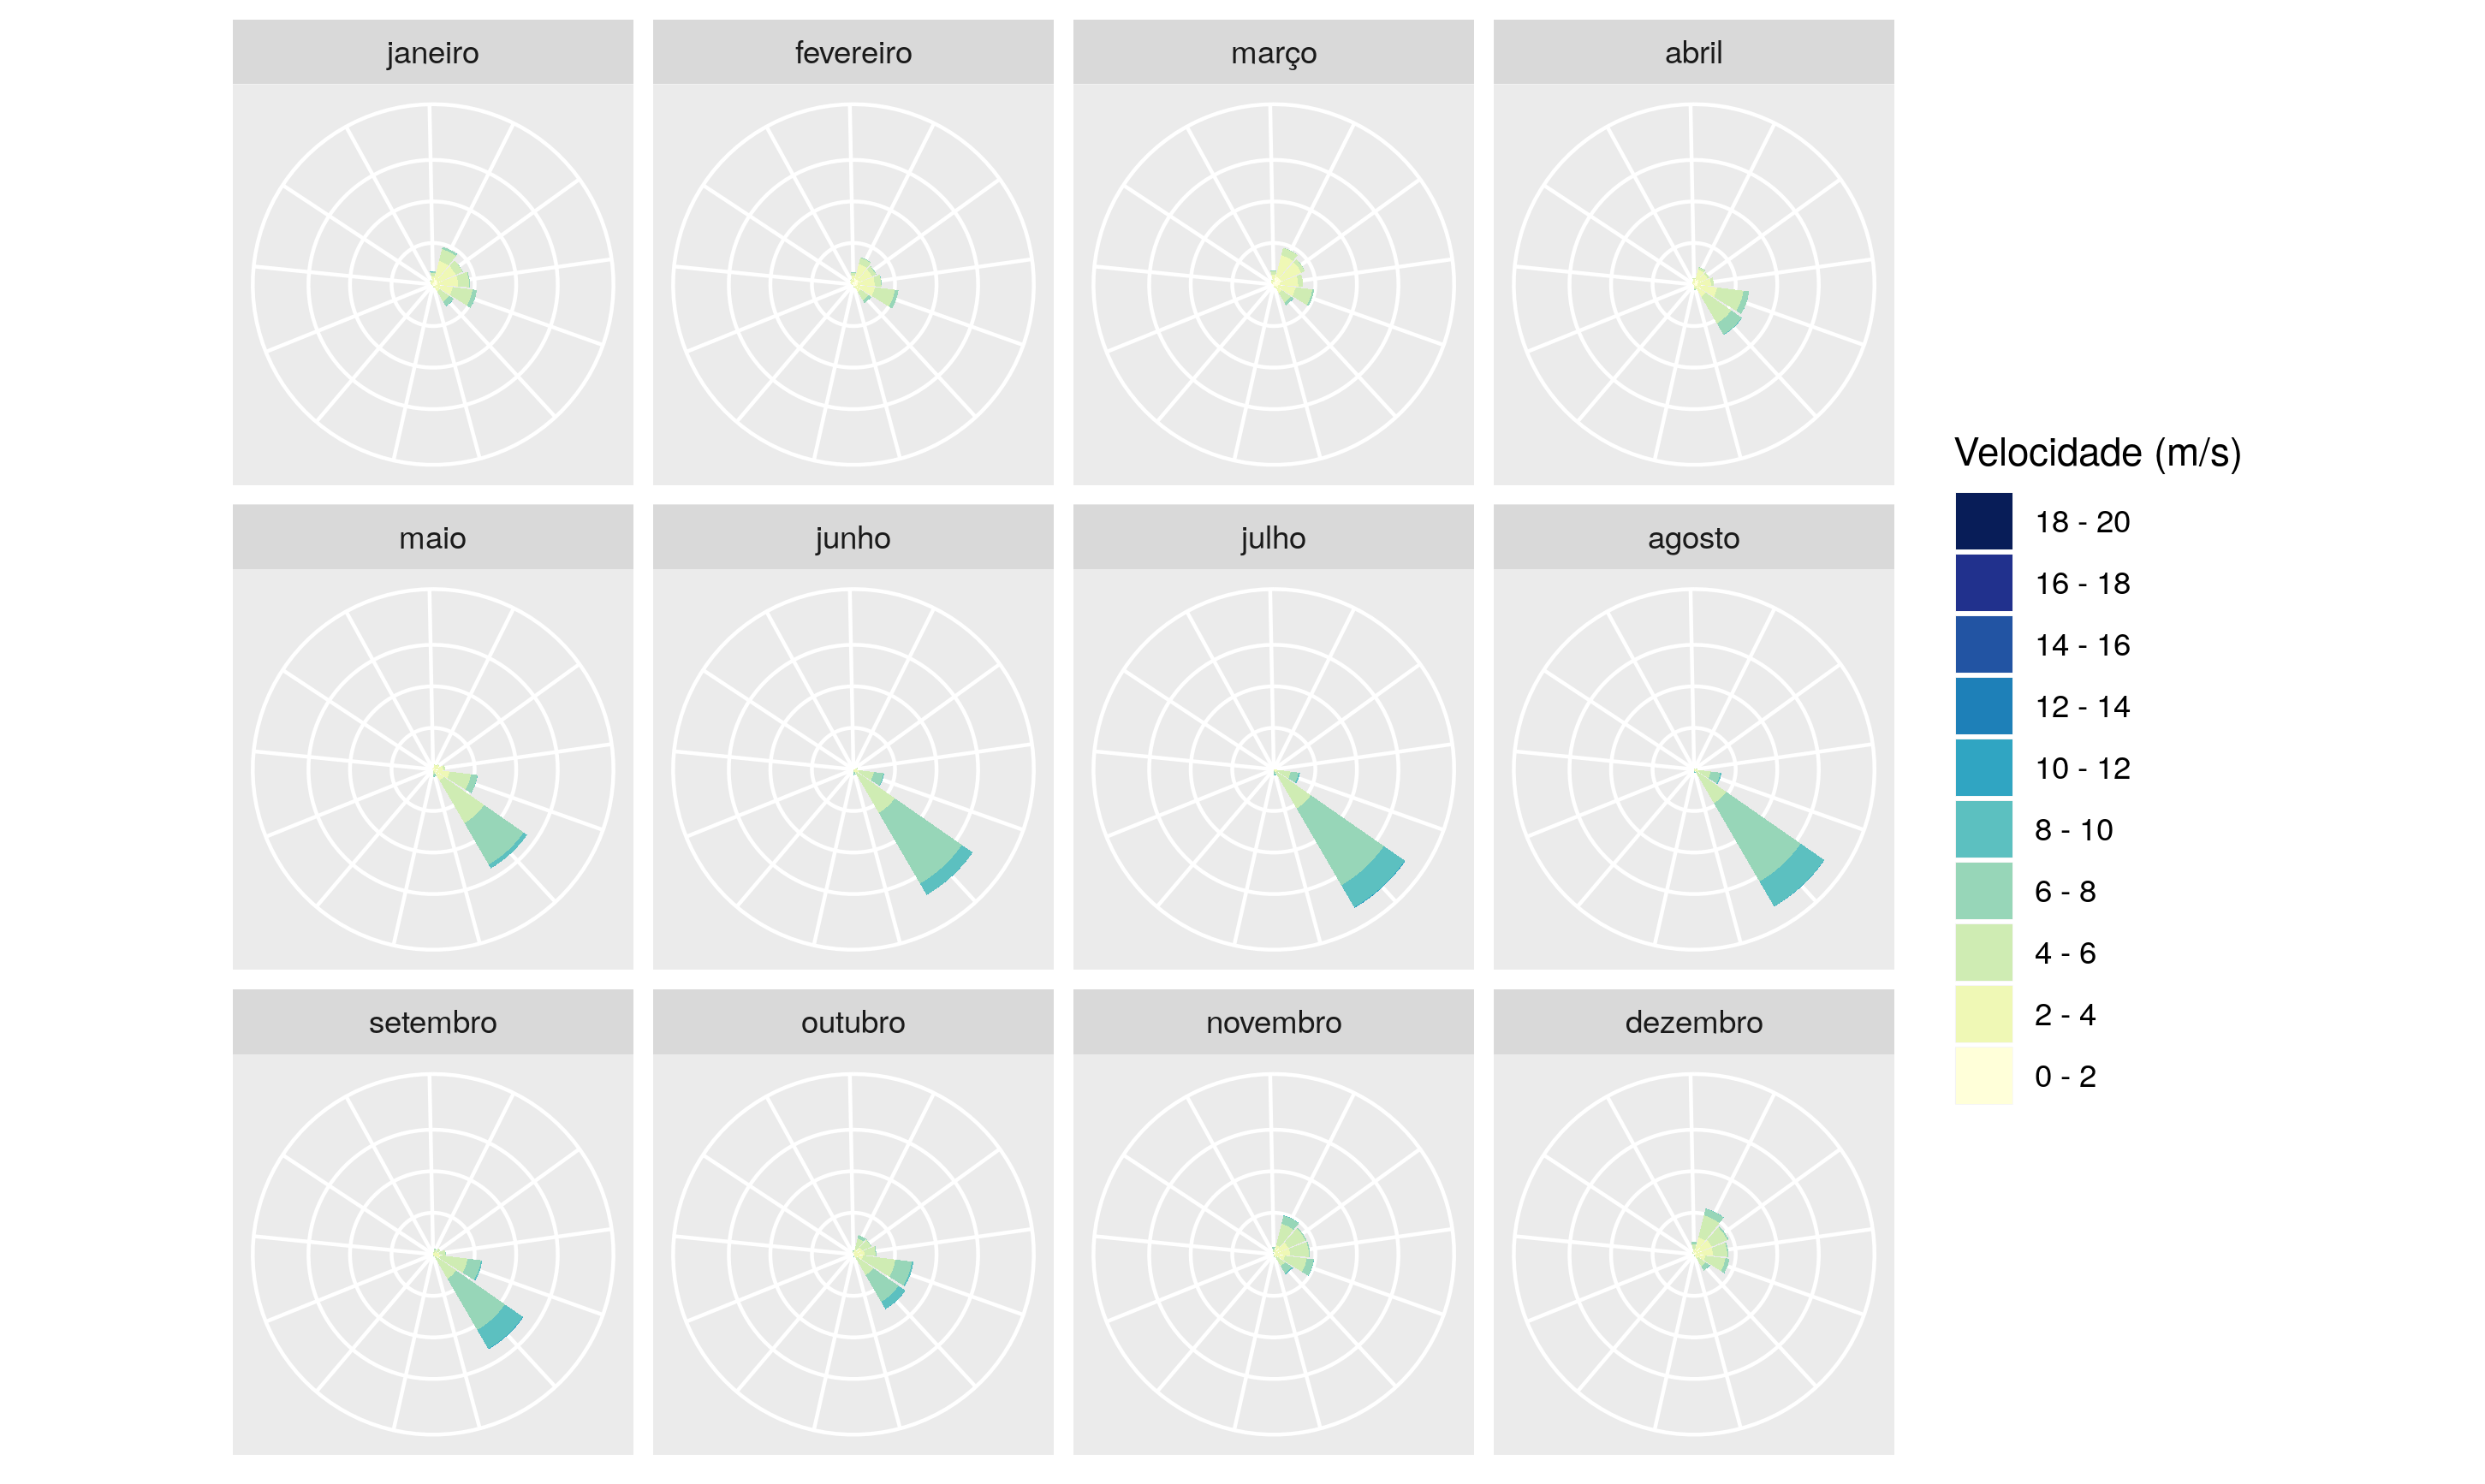
\includegraphics[scale=0.55]{windrose_monthly}
%		\caption{Rosas dos ventos mensais do recurso eólico da cidade de Sento Sé. Fonte: autoria própria, dados: ECWMF.}
%	\end{figure}
%}

%\begin{frame}
%	\frametitle{O Jogo do Caos}
%	\begin{columns}[t]
%		\column{.5\textwidth}
%		\centering
%		\fbox{\includegraphics[scale=0.5]{first}}\\
%		\vspace{0.5cm}
%		\fbox{\includegraphics[scale=0.5]{third}}\\
%		\column{.5\textwidth}
%		\centering
%		\vspace{0.5cm}
%		\fbox{\includegraphics[scale=0.5]{second}}
%		\fbox{\includegraphics[scale=0.5]{last}}
%	\end{columns}
%
%	\vspace{0.5cm}
%	O Jogo do Caos. Fonte: Wikimedia Commons. CC BY-SA 3.0
%\end{frame}

%\frame
%{
%	\frametitle{Triângulo de Sierpinski}
%	\begin{figure}[h]
%    	\centering
%		\includegraphics[scale=0.2]{triangle}
%		\caption{Triângulo de Sierpinski. Fonte: Wikimedia Commons. CC BY-SA 3.0}
%	\end{figure}
%}

%\frame
%{
%	\frametitle{O caráter estocástico do vento: anual}
%	\begin{figure}[h]
%	    \centering
%		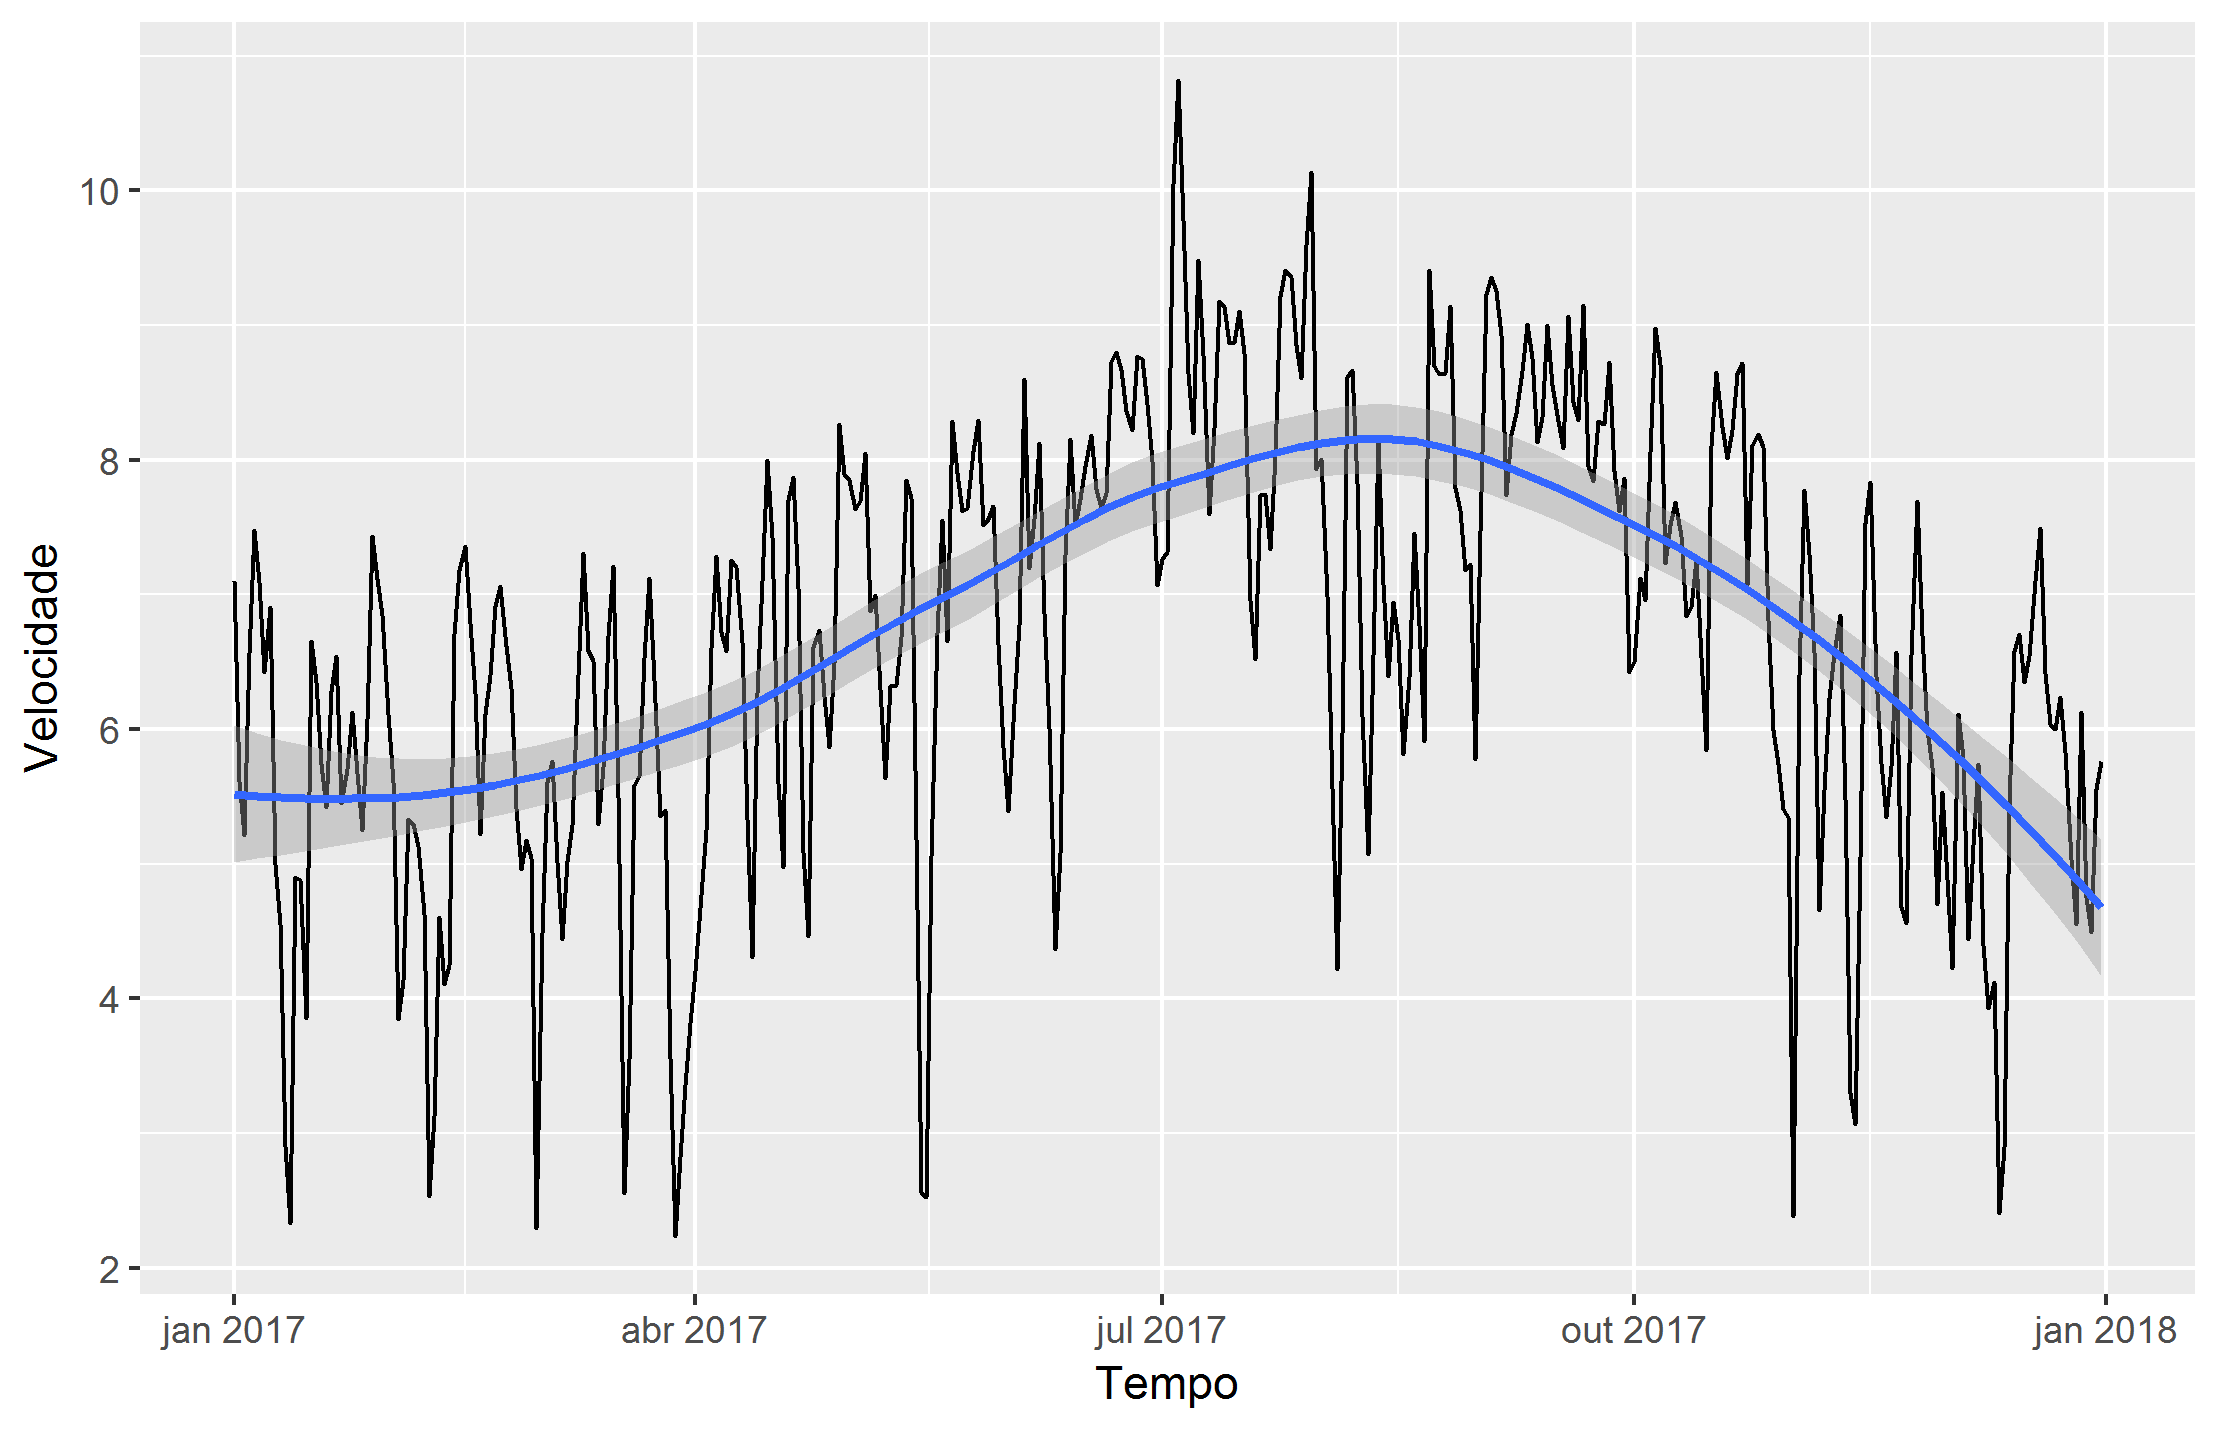
\includegraphics[scale=0.55]{stochastic}
%		\caption{Velocidade do vento medida por satélite na cidade de Sento Sé. Fonte: autoria própria. Dados: ECWMF. Curva em azul: ajuste aos dados medidos, dados: ECMWF}
%	\end{figure}
%}

%\frame
%{
%	\frametitle{O caráter estocástico do vento: mensal}
%	\begin{figure}[h]
%    	\centering
%		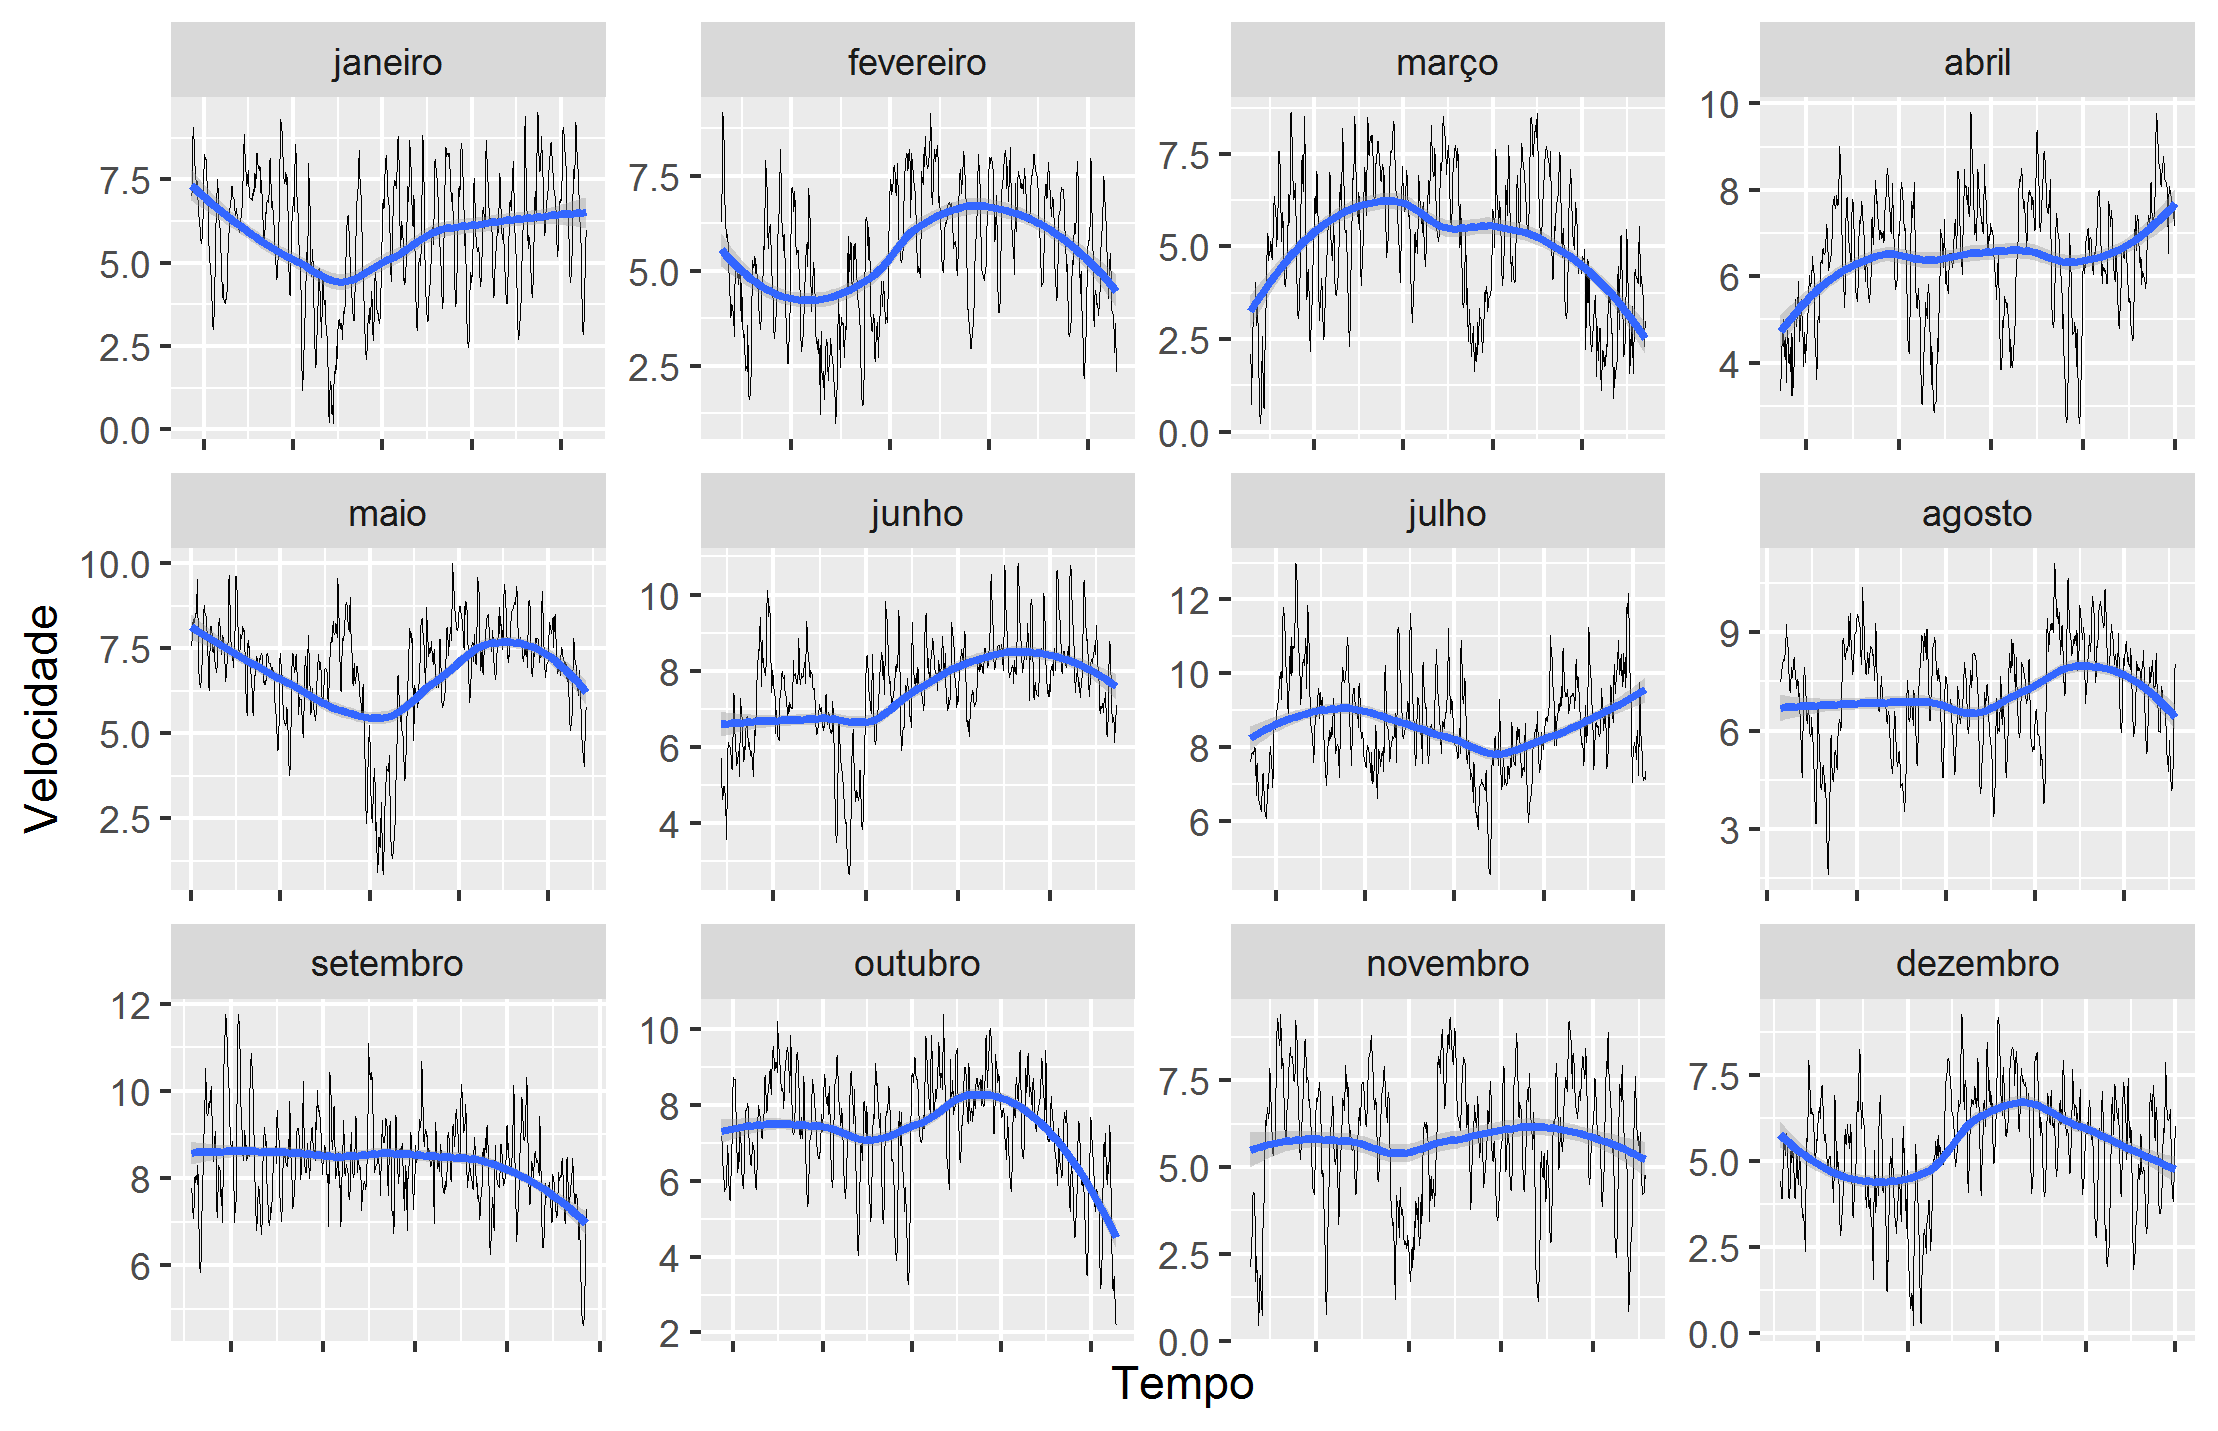
\includegraphics[scale=0.53]{stochastic_monthly}
%		\caption{Velocidade do vento para cada mês do ano de 2017 da cidade de Sento Sé no norte da Bahia. Curva em preto: dados medidos. Curva em azul: ajuste aos dados medidos. Fonte: autoria própria, dados: ECMWF.}
%	\end{figure}
%}

%\frame
%{
%	\frametitle{Ordem em meio ao caos}
%	\begin{figure}[h]
%	    \centering
%		\includegraphics[width=\textwidth]{diurnal}
%		\caption{Velocidade do vento para cada hora do dia e para cada mês do ano de 2017. Fonte: autoria própria, dados: ECWMF.}
%	\end{figure}
%}

%\frame
%{
%	\frametitle{Precisão numérica}
%	\begin{figure}[h]
%    	\centering
%		\includegraphics[scale=0.8]{grid}
%		\caption{Grid de medições. Fonte: Earth Magazine.}
%	\end{figure}
%}

%\frame
%{
%	\frametitle{Recurso eólico de longo prazo: distribuição de Weibull}
%	\begin{figure}[h]
%	    \centering
%		\includegraphics[scale=0.55]{weibull_histogram}
%		\caption{A distribuição de velocidades do quadrante central. Fonte: autoria própria, dados: ECWMF.}
%	\end{figure}
%}

%\frame
%{
%	\frametitle{Recurso eólico de longo prazo: distribuição de Weibull}
%	\begin{figure}[h]
%	    \centering
%		\includegraphics[scale=0.55]{weibull_freqpoly}
%		\caption{Distribuição de velocidades de todos os quadrantes. Fonte: autoria própria, dados: ECWMF.}
%	\end{figure}
%}

%\frame
%{
%    \frametitle{Resolução temporal}
%	Estimativa do recurso eólico em base mensal, diária, horária?
%	\begin{itemize}
%		\item 	mensal: negociação mais sólida com investidores
%		\item 	diária: minimizar perdas por manutenção
%		\item 	horária: adequamento da oferta de energia ao consumo local
%	\end{itemize}
%}

%\frame
%{
%	\frametitle{O cálculo estocástico na economia}
%	\begin{figure}[h]
%	    \centering
%		\includegraphics[scale=0.45]{stock}
%		\caption{Valor de abertura das ações da Google na NASDAQ. Curva em preto: dados medidos. Curva em azul: curva ajustada aos dados medidos. Fonte: autoria própria, dados: Google Finance.}
%	\end{figure}
%}

%\frame
%{
%	\frametitle{Proposta do trabalho}
%	\begin{block}{Objetivo}
%		Estimar a produção de energia, a partir de dados de vento, em curtos intervalos de tempo por meio de um modelo que contemple o caráter estocástico, físico, real do vento.
%	\end{block}
%}

%\frame
%{
%	\frametitle{Proposta do trabalho}
%	Para cumprir a proposta do trabalho é preciso:
%	\begin{itemize}
%		\item Fazer uma revisão da literatura
%		\item Entender fundamentos matemáticos: cálculo de Ito, teoria do caos, Monte Carlo
%		\item Entender os limites do estudo (precisão numérica, horizonte de previsão)
%		\item Simulação numérica
%		\item Entender como a estimativa de energia (de 20 anos) é feita
%		\item Comparação entre métodos e com dados medidos
%	\end{itemize}
%}

%\frame
%{
%	\frametitle{Planejamento}
%	\begin{figure}[h]
%		\hspace*{-0.8cm}   
%    	\includegraphics[scale=0.41]{gantt}
%	    \caption{Gráfico de Gantt do planejamento das etapas de desenvolvimento do presente trabalho. Fonte: autoria própria.}
%    	\centering
%	\end{figure}
%}

\end{document}
